\documentclass[handout, serif, aspectratio=169, 10pt]{beamer}

% packages
\usepackage{pxfonts}
\usepackage{setspace}
\usepackage{xcolor}

% table stuff
\usepackage{chronosys}
\usepackage{verbatim}
% \pagenumbering{arabic}
\usepackage{tabularx}
\usepackage{booktabs}
\usepackage{ragged2e}
\usepackage{mathtools}

% themes
\usetheme[progressbar=frametitle, block=fill]{metropolis}
\useoutertheme{metropolis}
\useinnertheme{metropolis}

% colors
\definecolor{dimwhite}{rgb}{0.99, 0.99, 0.99}
\definecolor{charcoal}{rgb}{0.21, 0.27, 0.31}
\definecolor{slategray}{rgb}{0.44, 0.5, 0.56}
\definecolor{dimgray}{rgb}{0.41, 0.41, 0.41}
\definecolor{bleudefrance}{rgb}{0.19, 0.55, 0.91}

% beamer options
\setbeamercolor{author}{fg=charcoal}
\setbeamercolor{background canvas}{bg=white}
\setbeamercolor{section in toc}{fg=charcoal}
\setbeamercolor{subsection in toc}{fg=dimgray}
\setbeamercolor{frametitle}{bg=dimwhite, fg=charcoal}
\setbeamercolor{progress bar}{fg=slategray, bg=fg!50!black!30}
\setbeamercovered{transparent}
\setbeamertemplate{itemize items}[triangle]
\setbeamertemplate{itemize subitem}[circle]
\setbeamertemplate{itemize subsubitem}[square]
\setbeamersize{text margin left=7mm,text margin right=7mm} 

% new commands
\newcommand{\q}[1]{``#1''}
\newcommand{\hs}[1]{\textsc{\hfill\scriptsize\color{dimgray}#1}}
\newcommand{\g}[1]{{\color{gray}#1}}
\newcommand{\dg}[1]{{\color{dimgray}#1}}
\newcommand{\sg}[1]{{\color{slategray}#1}}
\newcommand{\bdf}[1]{{\color{bleudefrance}#1}}
\newcommand{\itemcolor}[1]{\renewcommand{\makelabel}[1]{\color{#1}\hfil ##1}}
\newcommand\Wider[2][2em]{
\makebox[\linewidth][c]{
  \begin{minipage}{\dimexpr\textwidth+#1\relax}
  \raggedright#2
  \end{minipage}
  }
}

% misc
\linespread{1.35}

% Math stuff
\newcommand{\norm}[1]{\left\lVert#1\right\rVert}
\newcommand{\R}{\mathbb{R}}
\newcommand{\E}{\mathbb{E}}
\newcommand{\V}{\mathbb{V}}
\newcommand{\ol}{\overline}
%\newcommand{\ul}{\underline}
\newcommand{\pp}{{\prime \prime}}
\newcommand{\ppp}{{\prime \prime \prime}}
\newcommand{\policy}{\gamma}
\newcommand{\fp}{\frame[plain]}



% title page
\title{Common Ownership and Competition in the\\
 Ready-to-Eat Cereal Industry}
\author{Matt Backus, Chris Conlon, and Michael Sinkinson}
\institute{Berkeley Haas \& NBER, NYU Stern \& NBER, Yale SOM  \& NBER $\rightarrow$ Council of Economic Advisors}

\date{KU Leuven}




\begin{document}



%--------------
% TITLE PAGE
\begin{frame}[plain] %
\titlepage
\end{frame}



%--------------
% OVERVIEW

\begin{frame}[plain]{Today's Paper}
Two Research Questions
\begin{enumerate}
\item Applied: Do diversified investors with ownership stakes in multiple competitors \textit{cause} firms to compete less aggressively? (aka the \alert{Common Ownership Hypothesis})
\item Methodological: How can we look at observational data on prices and quantities and use instruments to determine which model of competition generated our data? (\alert{Conduct Testing}).
\end{enumerate}
\end{frame}



%------
% % TOC
% \begin{frame}[plain]{Roadmap}\vspace{0.25cm} %
% 	\linespread{0.75}
% 	\tableofcontents
% 	\vfill
% \end{frame}



%-------------
% SECTION 1
% \section{Testing Conduct}

% \begin{frame}[plain]{Conduct Testing in Industrial Organization}
% Foundational Empirical IO Question: How do we observe data on price and quantity and infer which model of firm behavior generated those outcomes?
% \pause
% \begin{itemize}
% \item Early work: Porter (1983), Bresnahan (1982,1987)
% \item Subsequent work defined the ``menu" approach: Nevo (1998, 2001), Villas-Boas (2007) 
% \item Recent revival of ``internalization'' parameters: Miller and Weinberg (2017), Crawford, Lee, Whinston, and Yurukoglu (2017), Pakes (2017)
% \item Subsequent work by: Duarte, Magnolfi, Sølvsten, Sullivan (2022) which test is best (RV). Magnolfi, Quint, Sullivan, Waldfogel (2022) Should we test or estimate?
% \item Applications of our test: Starc and Wollman (2022), Scuderi (2022), others?
% \end{itemize}
% Is conduct testable? Berry and Haile (2014): yes.
% \end{frame}

% \begin{frame}[plain]{Conduct Testing in Pictures (Berry Haile 2014)}
% \begin{center}
% 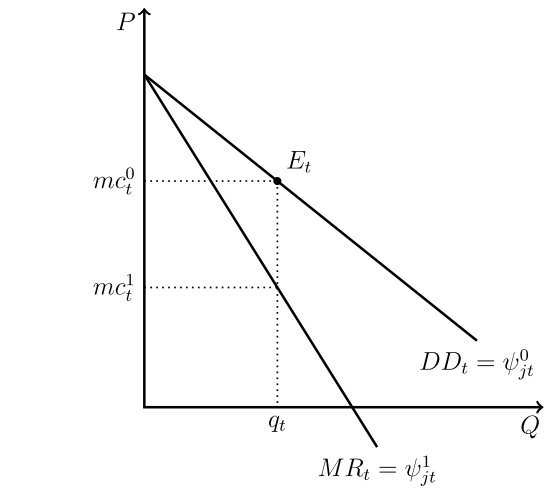
\includegraphics[width = 6.75cm]{figures/berryhaile1.png}
% 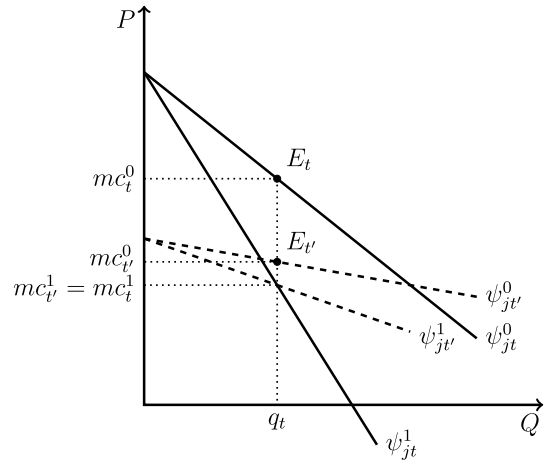
\includegraphics[width = 6.75cm]{figures/berryhaile2.png}
% \end{center}
% \small{Figure 2 from Berry and Haile (2014), Example 1.}
% \end{frame}

% \begin{frame}{Setup: Notation and Utility}
% We begin with a relatively standard BLP-style differentiated products setup.\\

% \begin{itemize}
%     \item Markets $t$
%     \item Products $j$
%     \item Data $\chi_t = \{(\textrm{x}_{jt},\textrm{v}_{jt},\textrm{w}_{jt})$ for all $j \in \mathcal{J}_t\}$ (characteristics of products)
%     \item Market Shares $\mathcal{S}_t = [s_{1t}, \ldots, s_{Jt}, s_{0t}]$.
%     \item Prices $\mathbf{p}_t = [p_{1t}, \ldots, p_{Jt}]$.
%     \item Consumers $i$ with demographics $y_{it}$ (income, presence of kids)
% \end{itemize}
% \end{frame}

% \begin{frame}{Basic Setup}
% We start with marginal revenue and marginal cost (unobserved $\omega$, observed $h(\cdot)$)
% \begin{align*}
% \psi_{jt}^{m} &= mc_{jt} \\
% p_{jt} -\eta_{jt}^m &= mc_{jt} \equiv h_s(\textrm{x}_{jt},\textrm{w}_{jt})  + \omega_{jt}^m
% \end{align*}
% \begin{itemize}
% \item Let's be vague/flexible with $h_s(\cdot)$ for now, but I don't know the production function.
% \item Assume: Demand and hence $\eta_{jt}^{m}$ are \alert{known (given conduct)}.\\
% \item Idea $(\eta^{A},\eta^{B})$ are monopoly/perfect competition or Cournot/Bertrand.
% \item Model is defined by a conditional moment restriction $\mathbb{E}[\omega_{jt}  | z_{jt}^s]=0$
% \end{itemize}
% \end{frame}



% \begin{frame}{The Question}
% Two competing markups $(\eta_{jt}^A, \eta_{jt}^B)$: which fits the data better?\\
% (both may be misspecified)
% \begin{align*}
% p_{jt} = h_s(\textrm{x}_{jt},\textrm{w}_{jt}) + \tau\, \eta_{jt}^A + (1-\tau)\,\eta_{jt}^B + \omega_{jt}
% \end{align*}
% Model is defined by a conditional moment restriction $\mathbb{E}[\omega_{jt}  | z_{jt}^s]=0$
% \begin{itemize}
% \item $H_0: \tau =1 \text{ vs } H_a: \tau = 0$
% \item This is a \alert{model selection} problem or a \alert{non nested testing} problem.
% \begin{itemize}
% \item We might want to compare more than two alternatives (too bad).
% \item Later: We test $A$ vs $B,C,D$ one at a time.
% \end{itemize}
% \item Obvious endogeneity problem with $\eta_{jt}(\chi_t, \omega_t)$!
% \end{itemize}
% \end{frame}


% \begin{frame}{Testing Environment}
% Compare violations of unconditional moments under $(\eta_{jt}^A, \eta_{jt}^B)$ and $A(z_{jt}^s)$:
% \begin{align*}
% p_{jt} -  \eta_{jt}^A = h_s(\textrm{x}_{jt},\textrm{w}_{jt}) + \omega_{jt}^{A}\\
% p_{jt} -  \eta_{jt}^B = h_s(\textrm{x}_{jt},\textrm{w}_{jt}) + \omega_{jt}^{B}
% \end{align*}
% \pause
% We are interested in GMM objective $Q_m = g_m'\, W_m\, g_m$ with:
% \begin{align*}
% g_A = \frac{1}{N} \sum_{jt} \omega_{jt}^{A}\, A(z_{jt}^s), &\quad
% g_B =\frac{1}{N} \sum_{jt}  \omega_{jt}^{B}\, A(z_{jt}^s)
% \end{align*}
% Now consider a \alert{Rivers Vuong (2002)} type test $T_{RV} = \sqrt{n} \left(\frac{Q_A - Q_B}{\sigma_{Q_A - Q_B}}\right) \sim N(0,1)$\\
% $H_0: Q_A - Q_B=0$ vs. $H_A: Q_A > Q_B$ or $Q_A < Q_B$.\\
% Getting the SD of the difference is hard $\rightarrow$ bootstrap 
% \end{frame}



% \begin{frame}{Comparison to Literature}
% \begin{itemize}
% \item Bresnahan (1987): Did LR test to determine collusion vs. competition in 1955 automobile price war
% \begin{itemize}
% \item No IV, errors were measurement in $P,Q$.
% \end{itemize}
% \item Bonnet and Dubois (2010): RV test
% \begin{itemize}
% \item But no IV -- maximum likelihood with normally distirbuted $\omega_{jt}$'s.
% \end{itemize}
% \item Villas Boas (2007): GMM/Cox test to determine double marginalization or not in yogurt
% \begin{itemize}
% \item Same IV as Demand: BLP IV plus wholesale milk price.
% \end{itemize}
% \item Duarte, Magnolfi, Sølvsten, Sullivan (2022): RV beats Cox pretty badly in Monte Carlo.
% \end{itemize}
% \end{frame}

% \begin{frame}{Setup: Challenges}
% The true model for markups (conduct) will satisfy the CMR: $\mathbb{E}[\omega_{jt} | z_{jt}^s]=0$
% \begin{align*}p_{jt} - \eta_{jt}^{(m)} &= h_s(\textrm{x}_{jt}, \textrm{w}_{jt}; \theta_3) + \omega_{jt}
% \end{align*}
% Goal is test two competing markups $\eta_{jt}^{(A)},\eta_{jt}^{(B)}$, but there are challenges:
% \pause
% \begin{enumerate}
% \item Test will depend on how we choose \alert{unconditional moment restrictions} $\mathbb{E}[\omega_{jt} \cdot \, A(z_{jt}^s)]=0$
% \pause
% \item Test may depend on how we specify $h_s(\cdot)$
% \begin{itemize}
% \item All tests are basically joint tests of the specification for \alert{observed marginal costs} and the  \alert{exclusion restriction}.
% \item Villas Boas (2007) tries log, linear, exponential in $x \beta $
% \end{itemize}
% \pause
% \item Choice of $\eta_{jt}^{(m)}$ will affect our choice of \alert{weighting matrix} and thus the test. (Hall Pelletier (2011))
% \end{enumerate}
% \end{frame}


% \begin{frame}[plain,label=chamberlain]{A Brief Aside: Chamberlain (1987) in a Slide}
% What contains as much information as the CMR $\mathbb{E}[\omega|z_{jt}^s]$ and moments of the form $ \mathbb{E}[\omega_{jt}\cdot A(z_{jt}^s)]. $
% \begin{itemize}
% \item For linear models $A(z_{jt}^s) = z_{jt}^s$ is generally without loss.
% \item For nonlinear models, Chamberlain (1987) shows that the efficient estimator uses
% $$A(z_{jt}^s) = \mathbb{E}\left[\frac{\partial \omega_{jt}}{\partial \theta}|z_{jt}^s\right]$$
% \item That is not too helpful (its a function of the unknown $\theta$).
% \item Much of the follow-up work has been about feasible approximations to this ``optimal instrument" (e.g., Newey 1990)
% \end{itemize}
% For us a similar concern arises, but it is about \alert{power} to distinguish conduct models rather than \alert{efficiency} of estimation.
% %\hyperlink{label=cmrbasics}{\beamerskipbutton{back}} 
% \end{frame}



% \begin{frame}[plain,label=innovation]{Our Idea: Motivation \#1 (Optimal IV)}
% The model is given by
% \begin{align*}
% p_{jt} &= h_s(\textrm{x}_{jt},\textrm{w}_{jt},\theta_3) + \tau \cdot \eta^A_{jt} + (1-\tau) \cdot \eta^B_{jt} + \omega^m_{jt}\\
% & \text{  where  }  H_0: \tau=1 \text{ and } H_a: \tau = 0
% \end{align*}

% \begin{itemize}
% \item The optimal IV in the Chamberlain (1987) sense is given by $\mathbb{E}\left[\frac{\partial \omega_{jt}}{\partial \tau}|z_{t} \right]= \mathbb{E}\left[\eta^A_{jt}-\eta_{jt}^B|z_{t}\right]$.
% \item In words: The IV need to predict the \alert{difference in markups}\\ (beyond observed $h_s(\textrm{x}_{jt},\textrm{w}_{jt},\theta_3)$).
% \end{itemize}
% \end{frame}




% \begin{frame}[plain,label=misspecification]{Our Idea: Motivation \#2 (Misspecification)}
% Index the \alert{true} model by $0$. Then,
% $$ p_{jt} -\eta^0_{jt}= h_s(x_{jt},w_{jt}) + \omega^0_{jt}.$$
% To motivate a useful test, we ask what happens when we estimate supply with the \alert{wrong} conduct model (1):
% \pause
% $$p_{jt} -\eta_{jt}^1 = h_s(x_{jt},w_{jt}) + \underbrace{\underbrace{\eta^0_{jt} - \eta^1_{jt}}_{\equiv \Delta \eta_{jt}^{0,1}} +  \omega_{jt}^{0}}_{\omega_{jt}^{1}}.$$
% \begin{itemize}
% \item Misspecifying conduct introduces an omitted variable: the difference in markups.
% \item Our test is premised on detection of this omitted variable.
% \end{itemize}
% % \hyperlink{advantages}{\beamerskipbutton{back}} 
% \end{frame}


% \begin{frame}[plain,label=innovation]{Our Innovation: How does this help?}
% % \begin{small}
% The model is given by
% $$p_{jt} - \eta^m_{jt} = h_s(\cdot) +  \omega^m_{jt} \text{,   and  } \mathbb{E}[\omega_{jt}^{(m)}\cdot A(z_t)] = 0.$$

% We suggest $A(z_t) = \mathbb{E}[\eta^1_{jt}-\eta_{jt}^2|z_{t}]$; several advantages:
% \pause
% \begin{itemize}
% % \item What is the point of instruments for testing? To explain the \alert{difference in markups}
% \item Reduces potentially many moments ($\mathbb{E}[\omega_{jt}' z_t]=0$) to a single, scalar moment. No need for a weighting matrix, or associated problems.
% \item Testing is reduced to two prediction exercises: $\mathbb{E}[\eta^1_{jt}-\eta_{jt}^2|z_{t}]$ and $\widehat \omega_{jt}^{(m)}$.
% \item Show in the Appendix that this maximizes $Q_1 - Q_2$ for a fixed weighting matrix.
% \item Downside: Our choice of instrument is \alert{pair specific}! UMP is not going to happen.
% \end{itemize}
% % \end{small}
% \end{frame}





% \begin{frame}{What about $z$?: Possible Exclusion Restrictions}
% \small
% We are looking for variables which affect \alert{demand but not supply}:
% \begin{align*}
% \sigma_{j}^{-1}(\mathcal{S}_t, \mathbf{p_t},\alert{\mathrm{y_t}}, \mathrm{x}_t,  \mathrm{v}_t, \widetilde{\theta}_2) 
% &= h_d(\mathrm{x}_{jt},\alert{ \mathrm{v}_{jt}}; \theta_1) - \alpha\, p_{jt} + \lambda \, \log(\text{ad}_{jt})+ \xi_{jt} \\
% p_{jt} - \eta_{jt}(\mathcal{S}_t, \mathbf{p_t}; \theta_2, \mathcal{H}_t(\kappa))
% &= h_s(\textrm{x}_{jt}, \alert{\mathrm{w}_{jt}}; \theta_3) + \omega_{jt} 
% \end{align*}
% Things we use:
% \begin{itemize}
%     \item Obvious choice: $\mathrm{v}_{jt}$ (things like product recalls are relatively weak)
%     \item Demographics (enter nonlinearly): $\mathrm{y}_t$ (chain-level income works well)
%     \item Characteristics of other goods: $f(\mathrm{x}_{-j,t})$ (BLP instruments).
%     \item Characteristics of other goods: $\mathrm{w}_{-j,t}$ (commodity price of oats for Rice Krispies)
% \end{itemize}
% \pause
% Things we don't use (but could):
% \begin{itemize}
%     \item Unobserved demand shocks $\xi_{jt}$ (see MacKay Miller 2020 for $Cov(\xi_j,\omega_j)=0$).
%     \item Observable $\kappa$ conduct shifters (financial mergers/events)
% \end{itemize}
% \end{frame}


% \begin{frame}[shrink=25,plain]{Algorithm}
% \begin{enumerate}[(1)]
% \item Split the sample by markets $t$ into 70\% \textit{test} and 30\% \textit{train}.
% \item On the \textit{training sample}:
% \begin{enumerate}[(a)]
% \item Approximate the optimal instruments $a(z_{jt}^s) = \mathbb{E}[\Delta \eta_{jt}^{(1,2)} \mid z_{jt}^s]$ as the fitted values from:
% \begin{align*}
%     \Delta\eta_{jt}^{1,2} = g(z_{jt}^s) + \zeta_{jt}.
% \end{align*}
% \item Estimate the marginal cost function, under models 1 and 2 to obtain residuals $\widehat{\omega_{jt}^{1}}$ and $\widehat{\omega_{jt}^{2}}$:
%  \begin{align*}
%  p_{jt} -\eta^m_{jt}= h_s(\textrm{x}_{jt},\mathrm{w}_{jt}; \theta_3) + \omega^m_{jt}.
%  \end{align*}
% \end{enumerate}
% \item On the \textit{test sample}:
% \begin{enumerate}[(a)]
% \item For each candidate model, compute the value of the scalar moment:\footnotemark
% \begin{align*}
%  Q(\eta^m) =\left(\sum_{j,t} \hat\omega_{jt}^m\cdot \hat{g}(\mathbf{z_t}) \right)^2.
% \end{align*}
% \item Repeat the previous step on bootstrapped samples and estimate $\hat\sigma/\sqrt{n}$ the standard error of the difference $\tilde Q(\eta^1) - \tilde Q(\eta^2)$.
% \item Compute the test statistic
% \begin{align*}
% T = \frac{\sqrt{n} \left(Q(\eta^1) -  Q(\eta^2) \right)}{\widehat{\sigma}} \sim \mathcal{N}(0,1).
% \end{align*}
% \textit{Note: Steps 2(a) and 2(b) can be done in any order via non-parametric regression.}
% \end{enumerate}
% \end{enumerate}
% \end{frame}

% \begin{frame}[plain]{Limitations}
% Not everything is testable:
% \begin{itemize}
% \item If $\Delta \eta_{jt}$ cannot be explained by $z_{jt}^s$ beyond contents of $(\mathrm{x}_j,\mathrm{w}_j)$ we have nothing
% \begin{itemize}
% \item We need a relevant overidentifying restriction!
%   \end{itemize}
% \item Flexible demand models are required to generate cross sectional variation in markups
% \item Beware of ``accidental'' exclusion restrictions.
% \end{itemize}
% \end{frame}



\section{What is Common Ownership?}

\begin{frame}[plain]{What is the Common Ownership Hypothesis?}
\begin{itemize}
\item Economics starts from the premise that firms maximize profits.
\begin{itemize}
\item Friedman (1953): natural selection of firms and billiards players.
\item Or, firms answer to investors, \alert{maximize shareholder value}.
\item We generally think of these objectives as aligned (possibly subject to managers' agency frictions).
\end{itemize}
\item So what do investors want?
\begin{itemize}
\item Some (diversified) investors may hold stakes in you \textit{and your competitor}. These are called ``common owners.''
\item Common owners are harmed when managers engage in \alert{business stealing}.
\end{itemize}
\item As a theory of firm behavior in \alert{joint ventures} this is an old idea. The recent innovation is to extend this approach to \alert{passive or institutional investors}
\end{itemize}
\end{frame}

\begin{frame}[plain]{Rise of the Big Three (S\&P 500 components, BCS AEJM 2021)}
\begin{center}
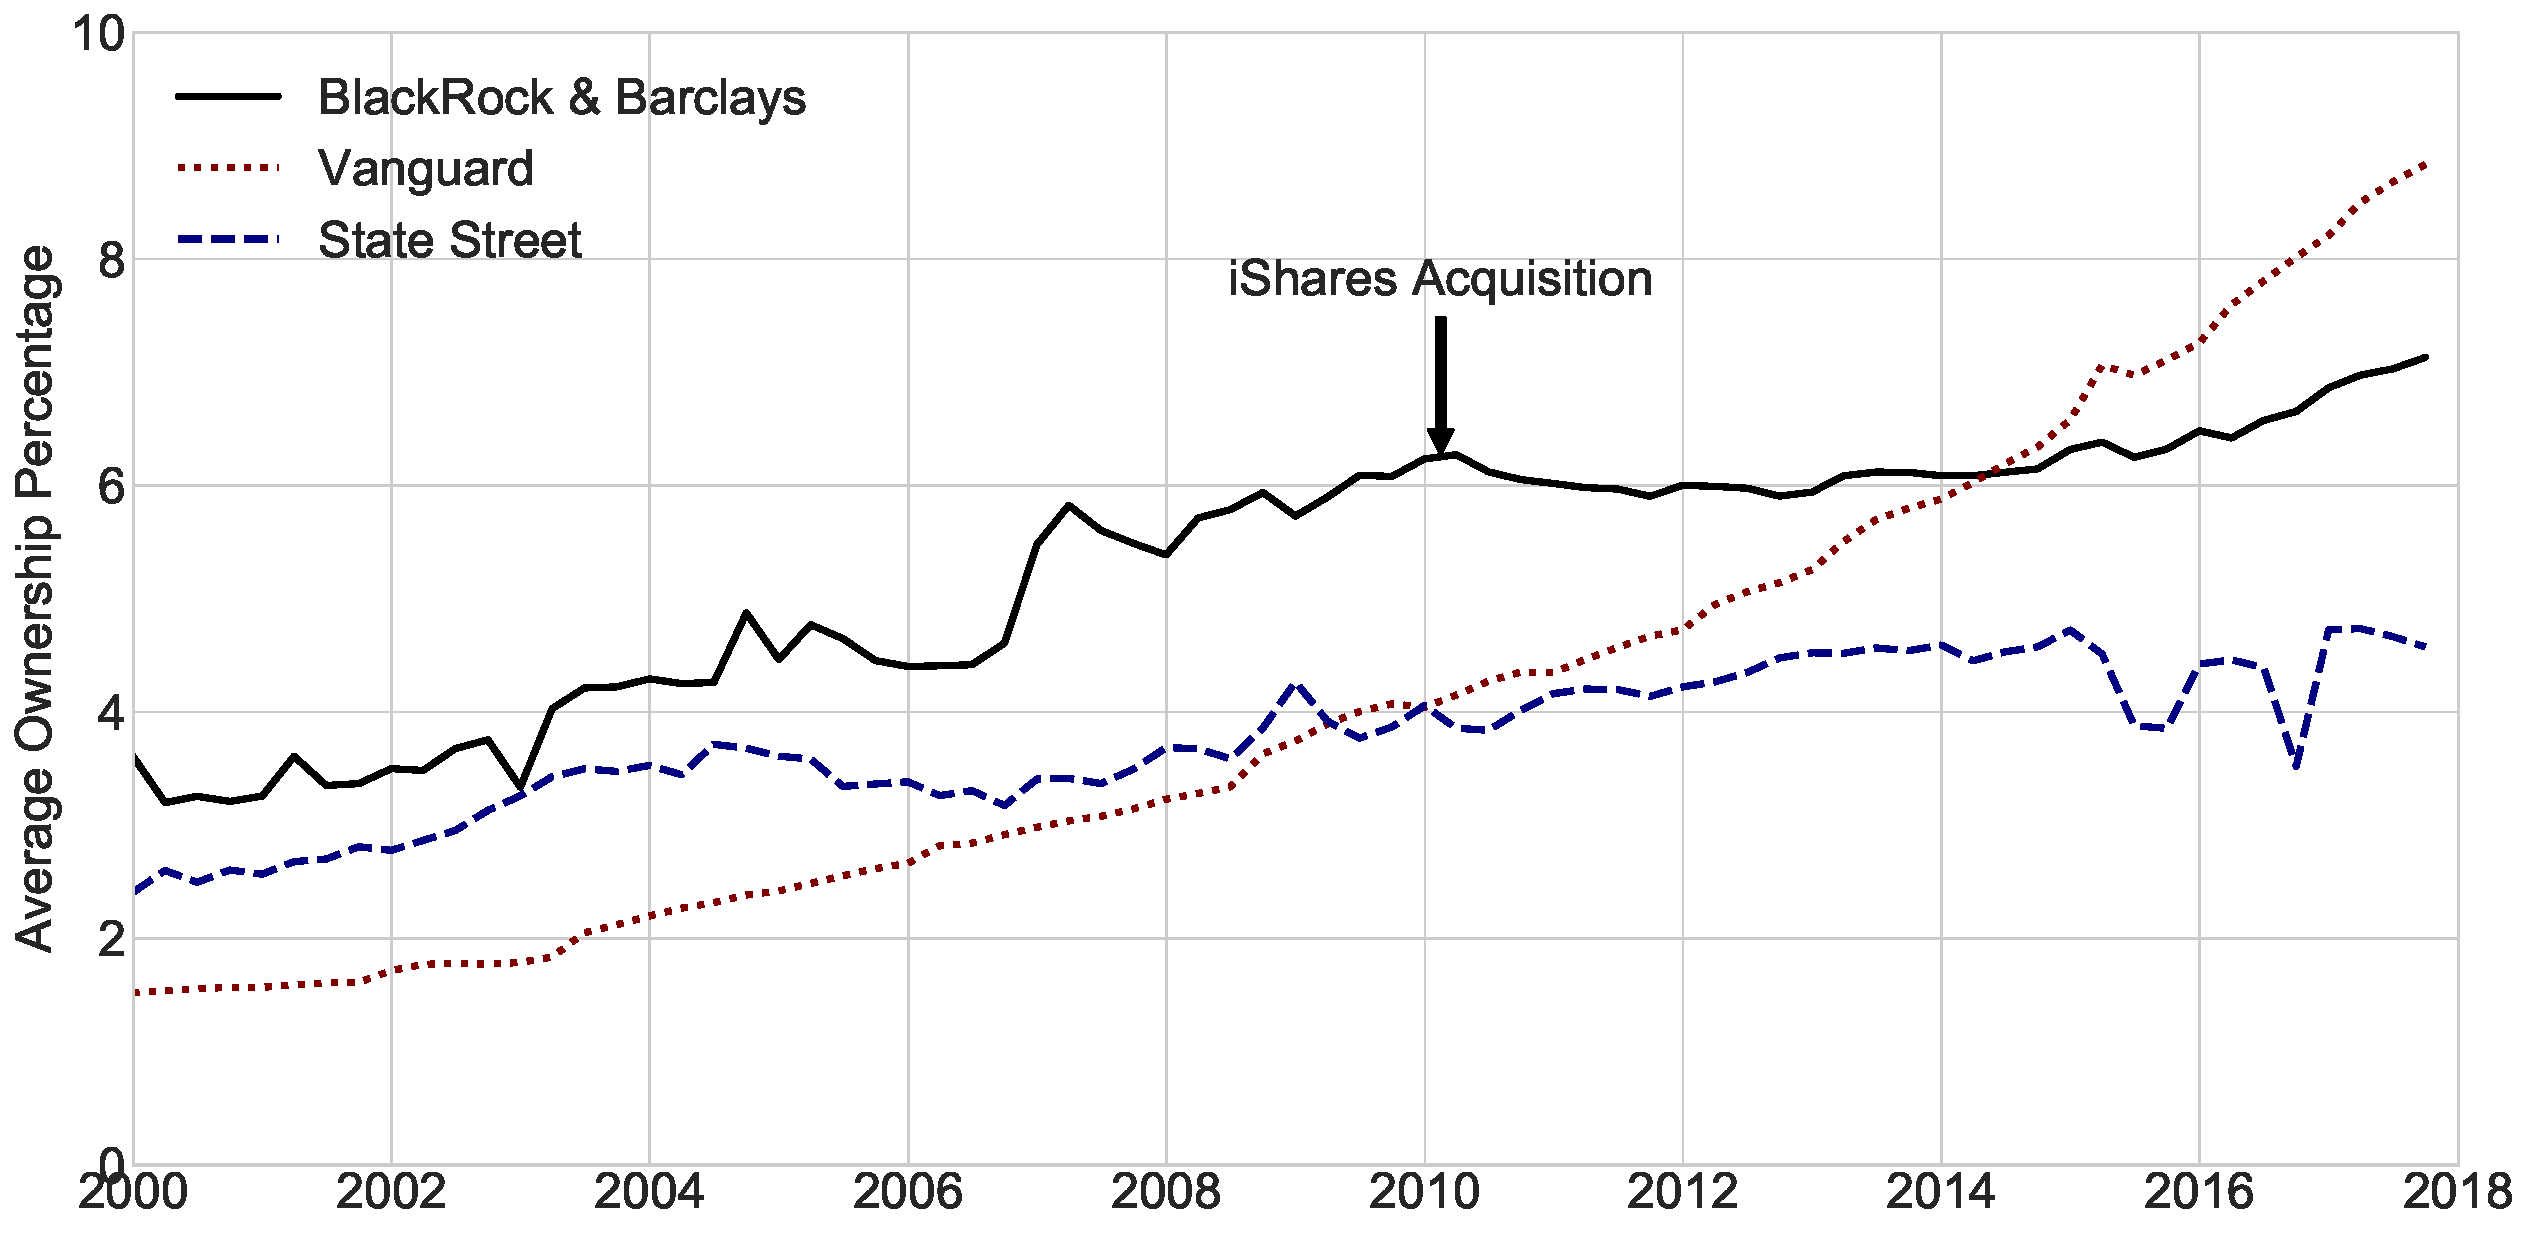
\includegraphics[height=0.9\textheight]{./figures/figure5_big3.pdf}
\end{center}
\end{frame}

\begin{frame}[plain]{Common Ownership in the News}
\begin{itemize}
\item The Atlantic: ``Are Index Funds Evil?"
\item The Economist: ``Stealth Socialism"
\item Bloomberg: ``Index-Crazed Investors Turning S\&P 500 Into One Gigantic Company"
\item MoneyWeek: ``Index Funds: Killing Capitalism?"
\item Reuters: ``When BlackRock Calls, CEOs Listen and do Deals"
\pause
\begin{itemize}
\item ``There is no CEO that doesn't return our call because typically we're up high on the shareholder register," Mark McCombe, global head of BlackRock's institutional client business, told Reuters reporters and editors attending the Reuters Global Wealth Management Summit on Friday.

``We are everybody's largest shareholder."
\end{itemize}
\end{itemize}
\end{frame}


\begin{frame}{Some Reasonable (?) Assumptions (BCS 2020 P\&P)}
Most models of common ownership (implicitly) make the following assumptions:
\begin{description}
\item[Investor Portfolios] Investors are entitled to a share of profits $\beta_{fs}$ and hold portfolios $V_s = \sum_{f} \beta_{fs} \pi_f$
\pause
\item[Manager Agency (Rotemberg 1984)] Managers maximize a $(\gamma)$ weighted average of investor payoffs $Q_f = \sum_{s} \gamma_{fs} V_s$.
\end{description}
These are pretty general since $s$ could contain the manager herself.\\
% Second one is more controversial.
\end{frame}

\begin{frame}{Derivation of Profit Weight}
\small
Easy to show:
\begin{align*}
Q_{f}\left(x_{f}, x_{-f}\right) &=\sum_{\forall s} \gamma_{f s} \cdot V_{s}\left(x_{f}, x_{-f}\right)\\
&\propto \pi_{f}+\sum_{g \neq f} \underbrace{\left(\frac{\sum_{\forall s} \gamma_{f s} \beta_{g s}}{\sum_{\forall s} \gamma_{f s} \beta_{f s}}\right)}_{\equiv \kappa_{f g}\left(\gamma_{f}, \beta\right)} \pi_{g}
\end{align*}
\begin{itemize}
    \item $\kappa_{fg}$ is interpreted as a \alert{profit weight}, where one dollar of profits at firm $g$ are valued as $\kappa_{fg}$ dollars in the objective function of firm $f$.
    \item Depends on two primitives: $\beta$ and $\gamma$.
\begin{itemize}
    \item $\beta$ (cash-flow rights) is often directly observable.
    \item $\gamma$ embeds a model of corporate governance. Literature assumes $\gamma = \beta$ (``proportional control").
\end{itemize}
\item Not specific to a particular strategic game.
\end{itemize}
\end{frame}

\begin{frame}[plain,label=simpleexample]{A Simple Example (with $\gamma = \beta$)}
\begin{itemize}
\item Firm 1 is controlled by an undiversified owner.
\item Firms 2 and 3 have symmetric structures:
\begin{itemize}
\item 60\% undiversified, retail investors with no influence ($\gamma = 0$)
\item 20\% two undiversified, institutional investors  ($\gamma = 0.5$)
\item 20\% commonly owned, institutional investor  ($\gamma = 0.5$)
\end{itemize}
\end{itemize}
Then,
$$
 \mathcal{H}(\kappa)= \begin{bmatrix}1 & 0 & 0 \\ 0 & 1 & 1/2 \\ 0 & 1/2 & 1\end{bmatrix}  
$$
%\hyperlink{kappainterp}{\beamerskipbutton{back}} 

\end{frame}

\begin{frame}[plain,label=strangeexample]
\frametitle{A Strange Example (still $\gamma = \beta$)}
\begin{itemize}
\item Firm 1 has
\begin{itemize}
\item $N$ diversified, symmetric institutional investors with $1\%$ each.
\item Undiversified retail investors ($\gamma = 0$) own remainder.
\end{itemize}
\item Firms 2 has 
\begin{itemize}
\item Same $N$ institutional investors with $x$\% each.
\item Undiversified retail investors ($\gamma = 0$) own remainder.
\end{itemize}
\end{itemize}
Then,
$$
\mathcal{H}\left(\kappa\right) = \begin{bmatrix}1 & x \\ \frac{1}{x} & 1\end{bmatrix}  
$$
%or $\kappa_{fg} = \frac{1- r_g}{1-  r_{f}}$ so that $\kappa$ grows with retail share $r$.
%\hyperlink{tunneling}{\beamerskipbutton{tunneling}} \hyperlink{kappainterp}{\beamerskipbutton{back}} 
\end{frame}


\begin{frame}[plain,label=kappaalt]{From BCS in AEJ:Micro (2021)}
\begin{center}
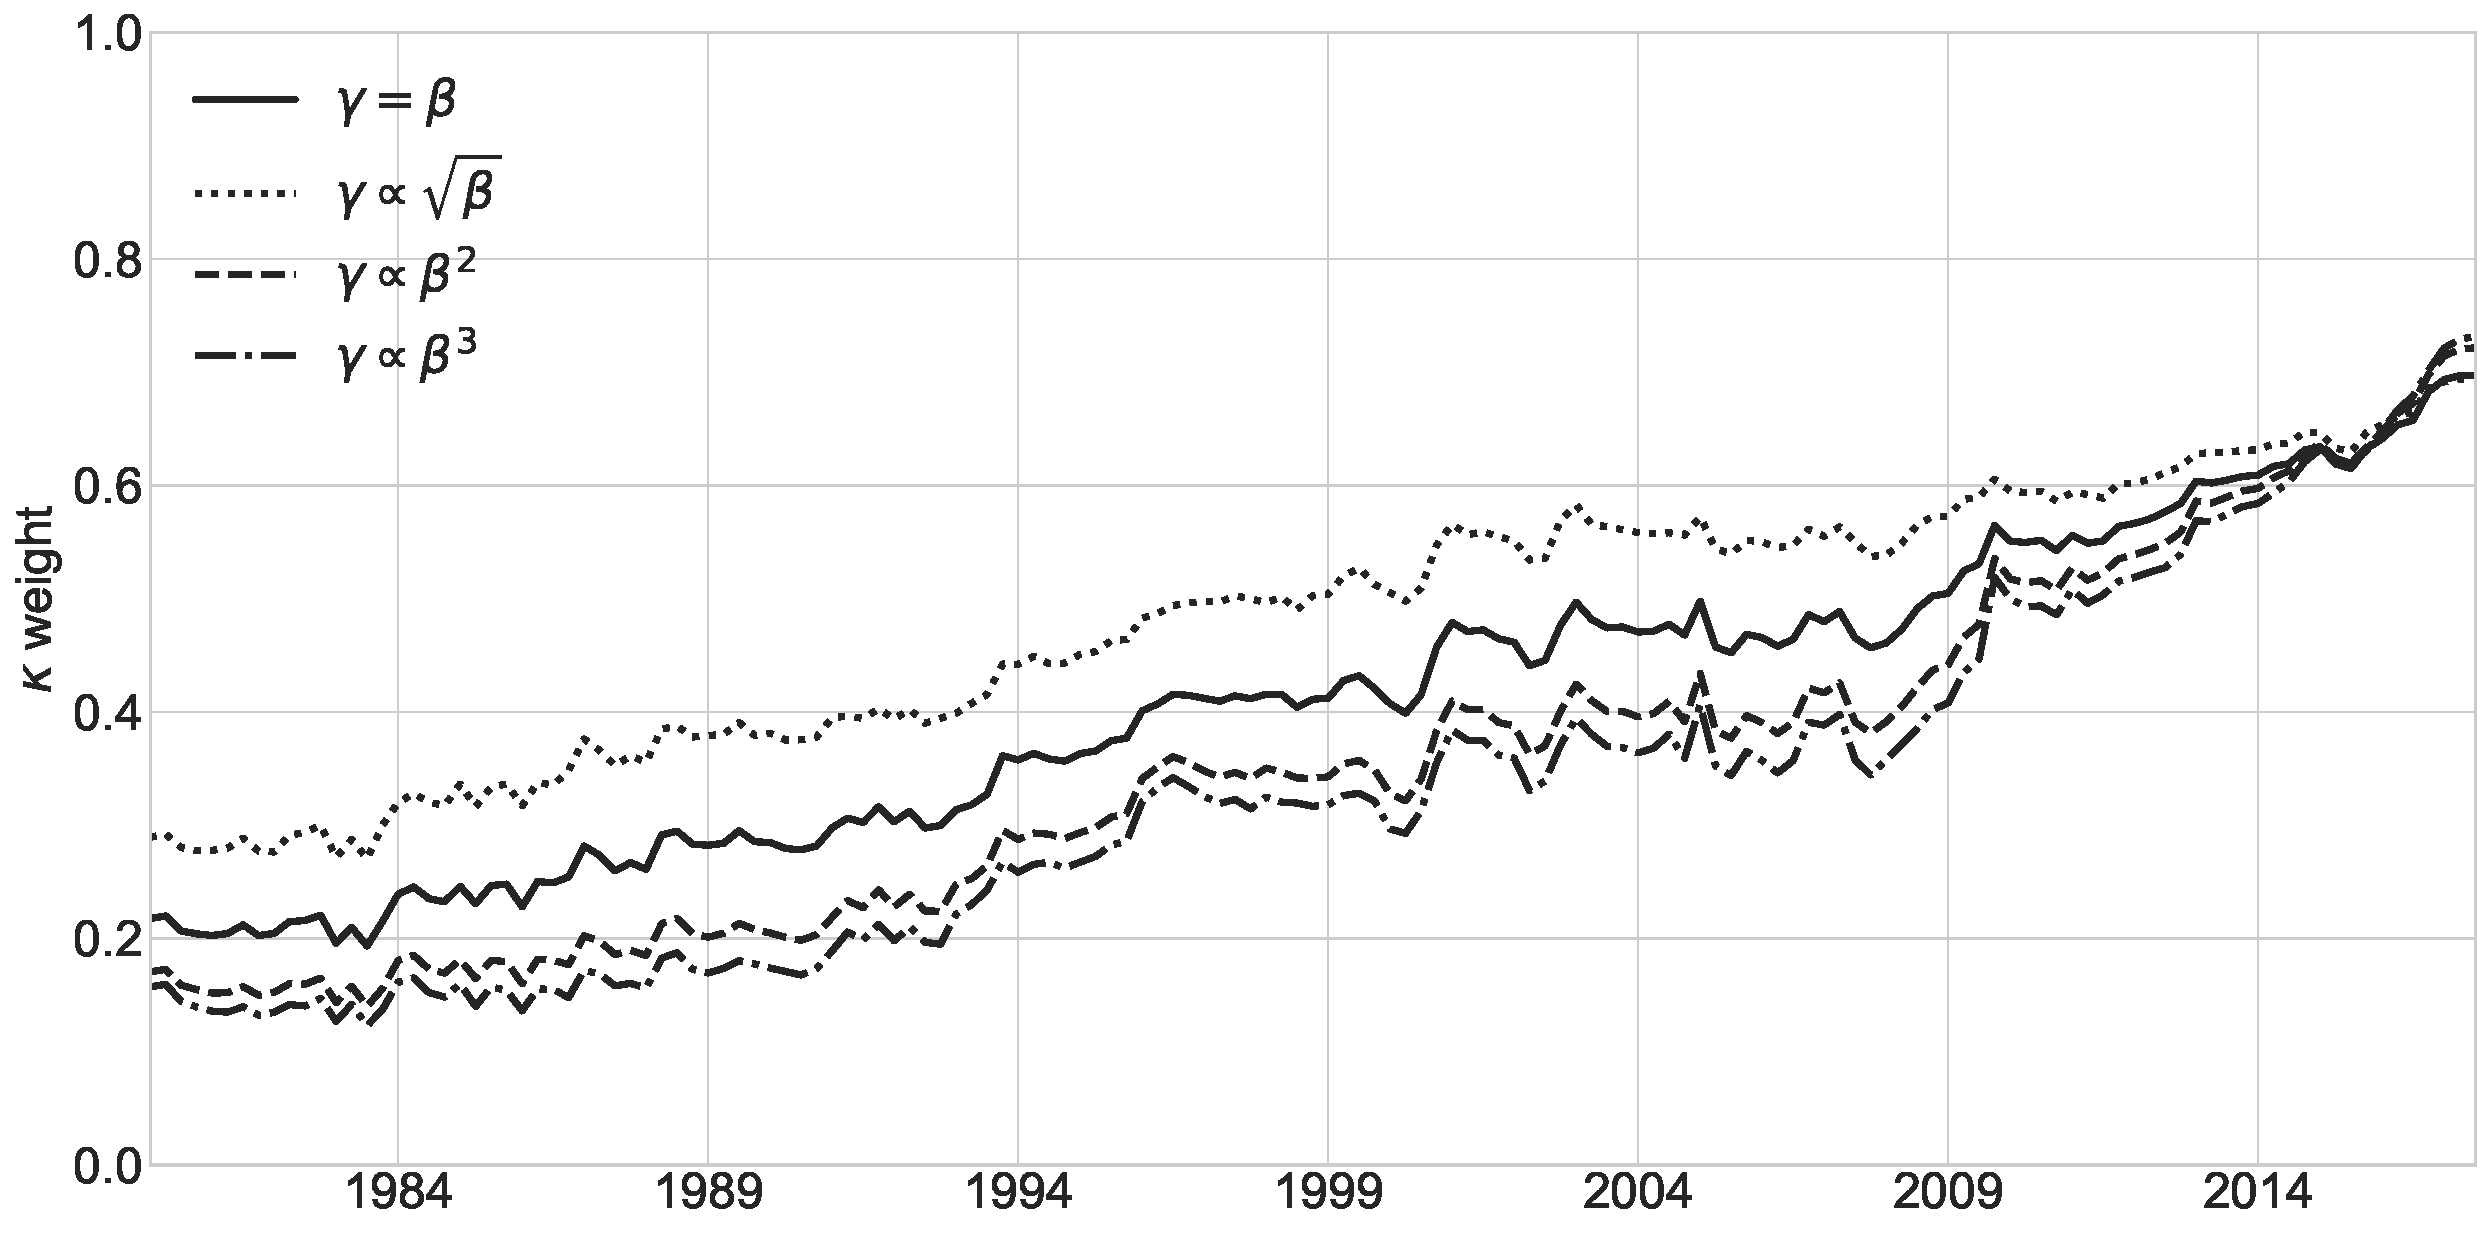
\includegraphics[height = 0.9\textheight ]{figures/figure13_kappa_control}
\end{center}
\end{frame}




\begin{frame}[plain,label=recoveringeta]{Aside: MHHI and (Symmetric, Homogenenous Good) Cournot}
\small
If instead firms choose quantities
 \begin{align*}
 \max_{q_f} \left (p(Q) - mc_f \right) \cdot q_f +  \sum_{g \neq f} \kappa_{fg} \cdot \left(p(Q) - mc_g \right) \cdot q_g
 \end{align*}
Gives share-weighted average markup:
\begin{align*}
\sum_f s_f \cdot \frac{p - mc_f}{p} &= \frac{1}{\eta} \sum_f \sum_g \kappa_{fg}\cdot s_f \cdot s_g \\
 MHHI &= \mathbf{s}' \, \mathcal{H}(\kappa) \, \mathbf{s}\\
 HHI &= \mathbf{s} \cdot \mathbf{s}\\
MHHID &= MHHI - HHI 
\end{align*}
Some regress
\begin{align*}
\log \left(p_{r j t}\right)=\beta \cdot M H H I \Delta_{r t}+\gamma \cdot H H I_{r t}+\theta \cdot X_{r j t}+\alpha_t+\nu_{r j}+\varepsilon_{r j t}
\end{align*}
 \end{frame}


\begin{frame}{Azar, Schmalz, Tecu (JF 2018)}

\begin{center}
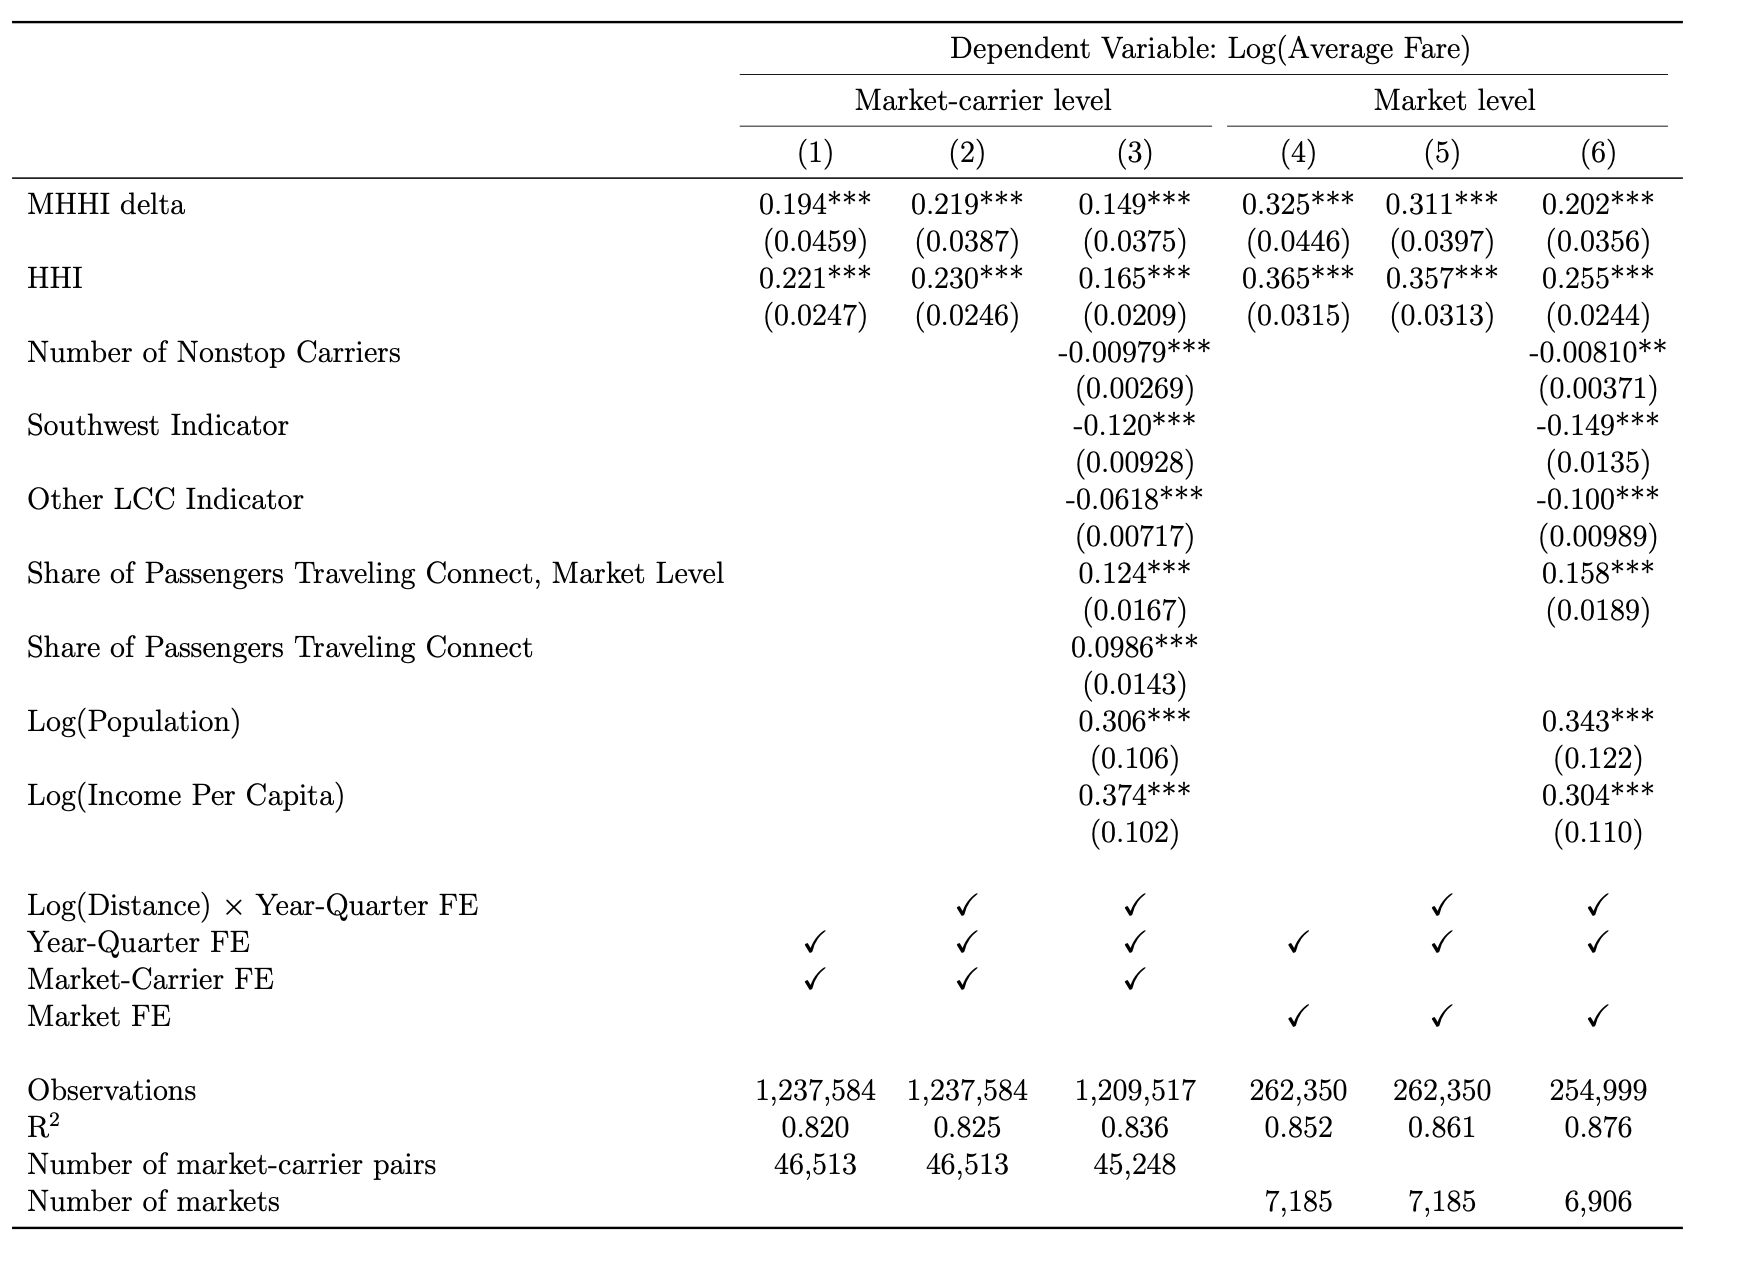
\includegraphics[height=0.95\textheight]{resources/ast_1.png}
\end{center}
\end{frame}


\begin{frame}[plain]{Common Ownership and Pricing: Bertrand}
Let $\kappa$ represent the weight a firm places on competitors. Starting with the objective function,
 \begin{equation*}
 \max_{p_j \,:\, j \in \mathcal{J}_f} \sum_{j \in \mathcal{J}_f} (p_j - mc_j) \cdot s_j(\mathbf{p})+
 \underbrace{\sum_{g\neq f} \kappa_{fg} \sum_{k \in \mathcal{J}_g} (p_k - mc_k) \cdot s_k(\mathbf{p})}_{\text{unique to CO}}
 \end{equation*}
 \pause
We obtain first order conditions 
 \begin{align*}
 s_j(p) + &  \frac{\partial s_j}{\partial p_j}(\mathbf{p})  \cdot (p_j - mc_j)
 + \sum_{k \in \mathcal{J}_f} \frac{\partial s_k}{\partial p_j}(\mathbf{p})  \cdot (p_k - mc_k)\\
 & +\underbrace{\sum_{g\neq f} \kappa_{fg} \sum_{k \in \mathcal{J}_g} \frac{\partial s_k}{\partial p_j}(\mathbf{p})  \cdot (p_k - mc_k)}_{\text{unique to CO}}=0.
  \end{align*}
\end{frame}



\begin{frame}[plain,label=recoveringeta]{From $\kappa$ to Markups}
A bit of notation, $\mathcal{H}$ is the product-level version of $\kappa$:
 \begin{equation*}
 \mathcal{H}_{jk}(\kappa) \equiv
 \begin{cases}
 1 & \text{if $(j, k) \in \mathcal{J}_f$ for any $f$,} \\
 \kappa_{fg} &  \text{if $j \in \mathcal{J}_f$ and $k \in \mathcal{J}_g$  for any $(f,g)$},\\
 0 & \text{otherwise. } \\
 \end{cases}f
 \end{equation*}
So that we can represent the system of first-order conditions where $\Omega_{jk}(\mathbf{p_t})) = -\frac{\partial q_k}{\partial p_j}$
  \begin{align*}
 \mathbf{s_t} &= (\mathcal{H}_t(\kappa) \odot \Omega(\mathbf{p_t})) \cdot (\mathbf{p_t} - \mathbf{mc_t}).
 \end{align*}
And therefore
 \begin{align*}
  \mathbf{mc_t} &= \mathbf{p_t} - \underbrace{(\mathcal{H}(\kappa) \odot \Omega(\mathbf{p_t}))^{-1} \mathbf{s_t}}_{\equiv\eta(\mathbf{p},\mathbf{s},\mathcal{H}(\kappa))}.
 \end{align*}
 \end{frame}




\begin{frame}[plain]{Common Questions about Common Ownership}
\begin{enumerate}
\item Isn't this just a partial-merger? (Yes).
\item In some cases (like double marginalization) don't partial-mergers better align incentives? (Yes).
\item Can we have $\kappa > 1$? (Yes). What does that mean? (Firms value own profits less than rivals, and have incentive to \alert{tunnel}$\rightarrow$ see BCS AEJ 2021).
\item What about an alternative for $\gamma$? Banzhaf Power, Voting Models, etc. (Sure, but remember Arrow says microfounding social choice is hard).
\end{enumerate}
 \end{frame}




\begin{frame}[plain]{What about the mechanism?}
\begin{itemize}
\item In some sense this is a \alert{frictionless} model
\begin{itemize}
  \item Managers do exactly what investment managers want
  \item Investment managers seek to maximize \alert{portfolio value}
\end{itemize}
\item Some attempts at micro foundations are questionable
\begin{itemize}
  \item Anton, Ederer, Gine, Schmalz: toy model has manager choose effort to reduce $MC$.
  \item Weaker managerial incentives: higher $MC$ and higher $P$
  \item Some correlation that executives at commonly owned firms have peformance less correlated with profitability.
\end{itemize}
\end{itemize}
 \end{frame}




\section{Why Cereal?}

\begin{frame}{Many Reasons}
Long history in IO ``model organism'', but also non-Nash behavior isn't so crazy:
\begin{itemize}
\item Market structure: 4 big firms
\item Nevo x 3
\item FTC Case in the 1970's (Schmalensee 1978)
\item Post/Nabisco Merger case (Rubinfeld 2000)
\item Cartel/Price War in 1990s (Michel Weierergraeber 2022)
\end{itemize}
\end{frame}


\begin{frame}{Cereal Data}
Main Dataset is NielsenIQ (from Kilts) from 2007-2017
\begin{itemize}
\item Consolidate to \texttt{dma-chain-week}.
\item Keep largest chains who price at chain level
\begin{itemize}
\item Select based on \# observations from panelist data.
\end{itemize}    
\item Consolidate \texttt{upc} $\rightarrow$ \texttt{brand} (Honey Nut Cheerios) from multiple package sizes and box designs.
\begin{itemize}
\item Divide revenue by servings
\item Maintain the fiction that households purchase servings.
\end{itemize}
\end{itemize}
\end{frame}


\begin{frame}[plain]{Cereal Data: Variation in $\kappa$}
\begin{center}
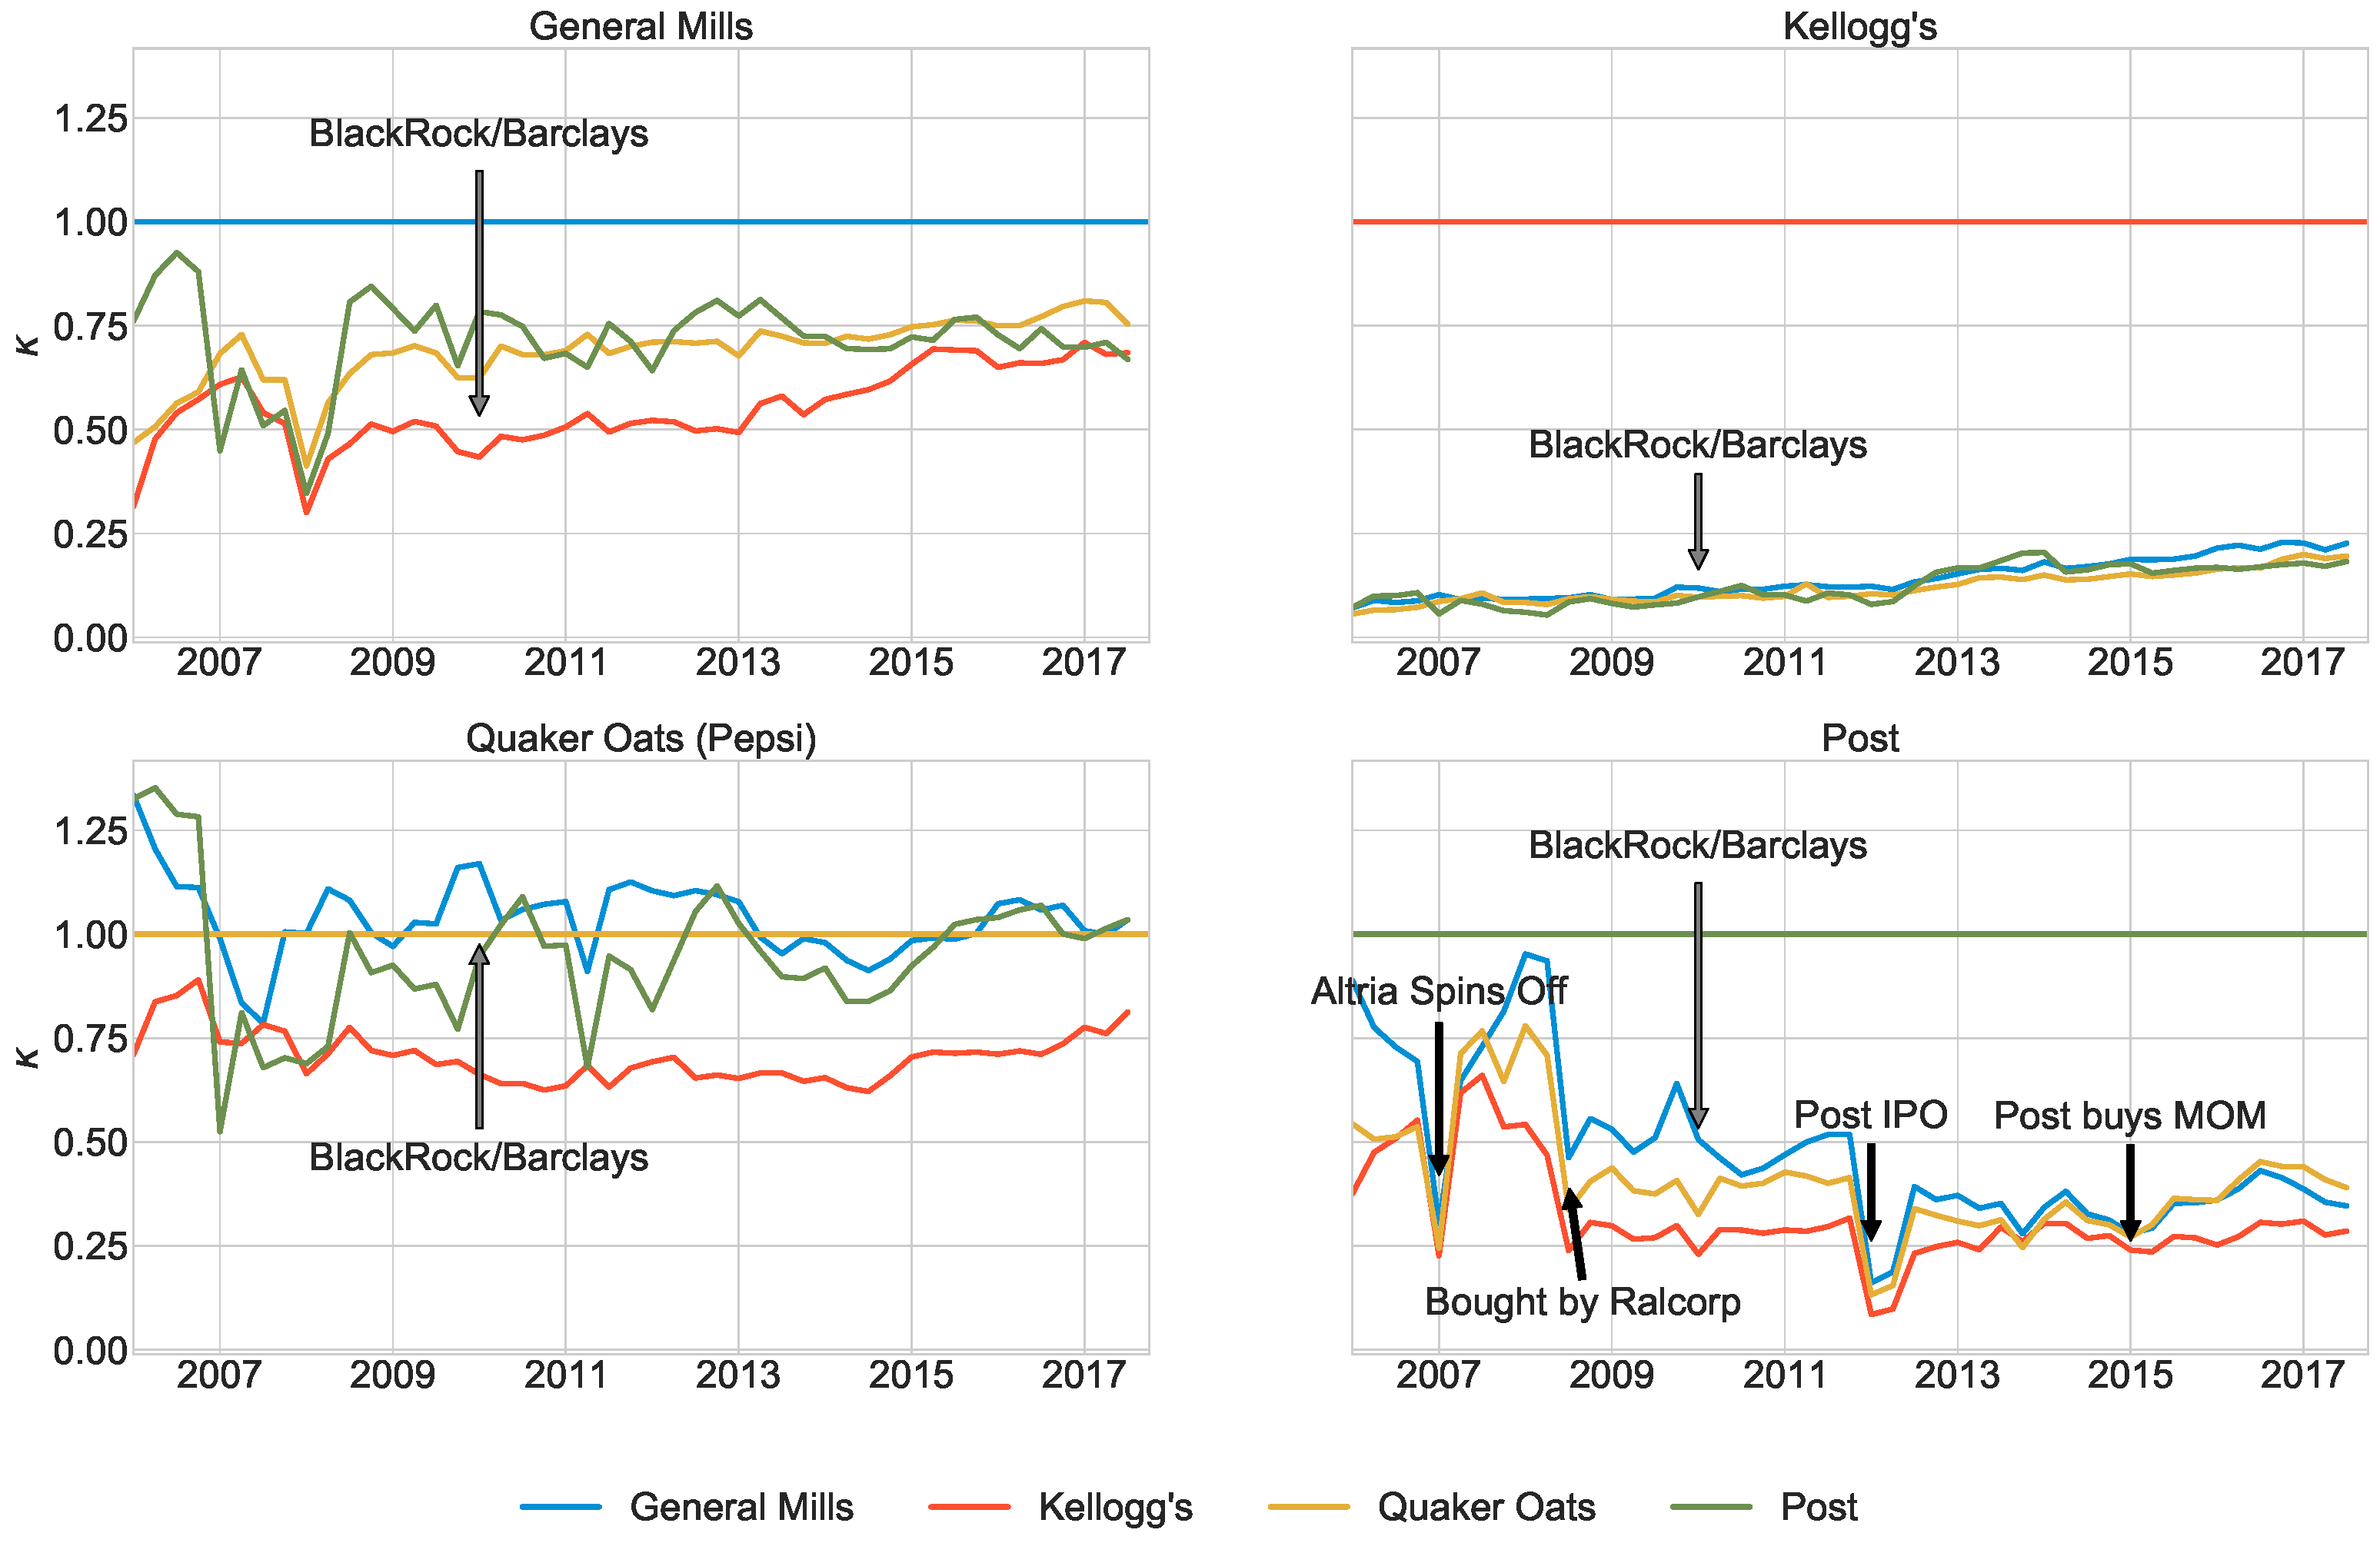
\includegraphics[height = 0.9\textheight ]{figures/cereal_kappas_alpha_1.pdf}
\end{center}
\end{frame}


\begin{frame}{Foreshadowing}
\begin{itemize}
\item Kellogg's should be a \alert{maverick} who ignores cooperation from rivals and cares about own profit.
\begin{itemize}
\item Instead they are the highest priced (margin) firm or are uniquely inefficient.
\end{itemize}
\item Quaker Oats (Pepsi) should want to \alert{tunnel} profits to rivals when $\kappa > 1$ and possibly price into inelastic part of demand curve.
\begin{itemize}
\item They seem to be a low margin tough competitor. (or their mc is zero).
\end{itemize}
\item Post should \alert{cut prices} sharply around large decreases in $\kappa$ (de-listing events).
\begin{itemize}
\item Actually they tend to \alert{raise prices} around those times.
\end{itemize}
\end{itemize}
\end{frame}



\begin{frame}[plain]
\frametitle{The ``Forbidden" Slide}
\begin{center}
\scalebox{.6}{{
\def\sym#1{\ifmmode^{#1}\else\(^{#1}\)\fi}
\begin{tabular}{l*{6}{c}}
\hline\hline
                    &\multicolumn{1}{c}{(1)}   &\multicolumn{1}{c}{(2)}   &\multicolumn{1}{c}{(3)}   &\multicolumn{1}{c}{(4)}   &\multicolumn{1}{c}{(5)}   &\multicolumn{1}{c}{(6)}   \\
                    &  Log(Price)   &  Log(Price)   &  Log(Price)   &  Log(Price)   &  Log(Price)   &  Log(Price)   \\
                    &        b/se   &        b/se   &        b/se   &        b/se   &        b/se   &        b/se   \\
\hline
hhi\_servings        &      0.0495***&      0.0857***&     -0.0105   &      0.0181***&      0.0578***&      0.0559***\\
                    &    (0.0068)   &    (0.0074)   &    (0.0066)   &    (0.0064)   &    (0.0057)   &    (0.0060)   \\
mhhid\_os\_servings   &     -0.1216***&     -0.1204***&     -0.1523***&     -0.1097***&     -0.0833***&     -0.0892***\\
                    &    (0.0079)   &    (0.0081)   &    (0.0065)   &    (0.0064)   &    (0.0056)   &    (0.0059)   \\
share\_servings      &               &               &               &               &     -0.0116***&     -0.0117***\\
                    &               &               &               &               &    (0.0003)   &    (0.0003)   \\
DMA FEs             &          No   &         Yes   &          No   &         Yes   &         Yes   &         Yes   \\
Retailer FEs        &          No   &          No   &         Yes   &         Yes   &         Yes   &         Yes   \\
Quadratic Time Trend &         Yes   &         Yes   &         Yes   &         Yes   &         Yes   &         Yes   \\
Parent FEs          &         Yes   &         Yes   &         Yes   &         Yes   &         Yes   &         Yes   \\
Cubic HHI           &          No   &          No   &          No   &          No   &          No   &         Yes   \\
\hline
r2\_a                &       0.267   &       0.312   &       0.722   &       0.754   &       0.814   &       0.814   \\
N                   &        5173   &        5173   &        5173   &        5173   &        5173   &        5173   \\
\hline\hline
\multicolumn{7}{l}{\footnotesize * p<0.10, ** p<0.05, *** p<0.01}\\
\end{tabular}
}
}
\end{center}
\scriptsize Both $HHI$ and $MHHI$ scaled for 1000 point increase.
\end{frame}

\section{Empirical Application}

\begin{frame}{Implementation: Demand Specification}
\begin{gather*}
u_{ijt} =  h_d(\textrm{x}_{jt}^{(1)}, \textrm{v}_{jt}; \theta_1) - \alpha\, p_{jt} + \lambda \, \log(\text{ad}_{jt})  + \left(\Sigma \, \nu_i + \Pi\, y_i \right) \cdot x_{jt}^{(2)}+ \xi_{jt} + \varepsilon_{ijt}\\
\end{gather*}
\vspace{-0.75cm}
\begin{itemize}
\item $y_i$ demographics: estimated at the $\texttt{dma-chain-year}$ level (from panelists)
\item $y_i$ is joint distribution of $(income, kids)$
\begin{enumerate}
\item Fit a lognormal for income to households w/ and w/o kids.
\end{enumerate}
\item $\nu_i$ are random (normal) draws; price is lognormal.
\item Lots of FE in $h_d(\cdot)$ (product, chain-dma, year, week of year)
\item IV: Cost shifters, GH/Optimal IV $f(x_{-j})$, lagged advertising.
\end{itemize}
\end{frame}

\begin{frame}[plain]
\begin{center}
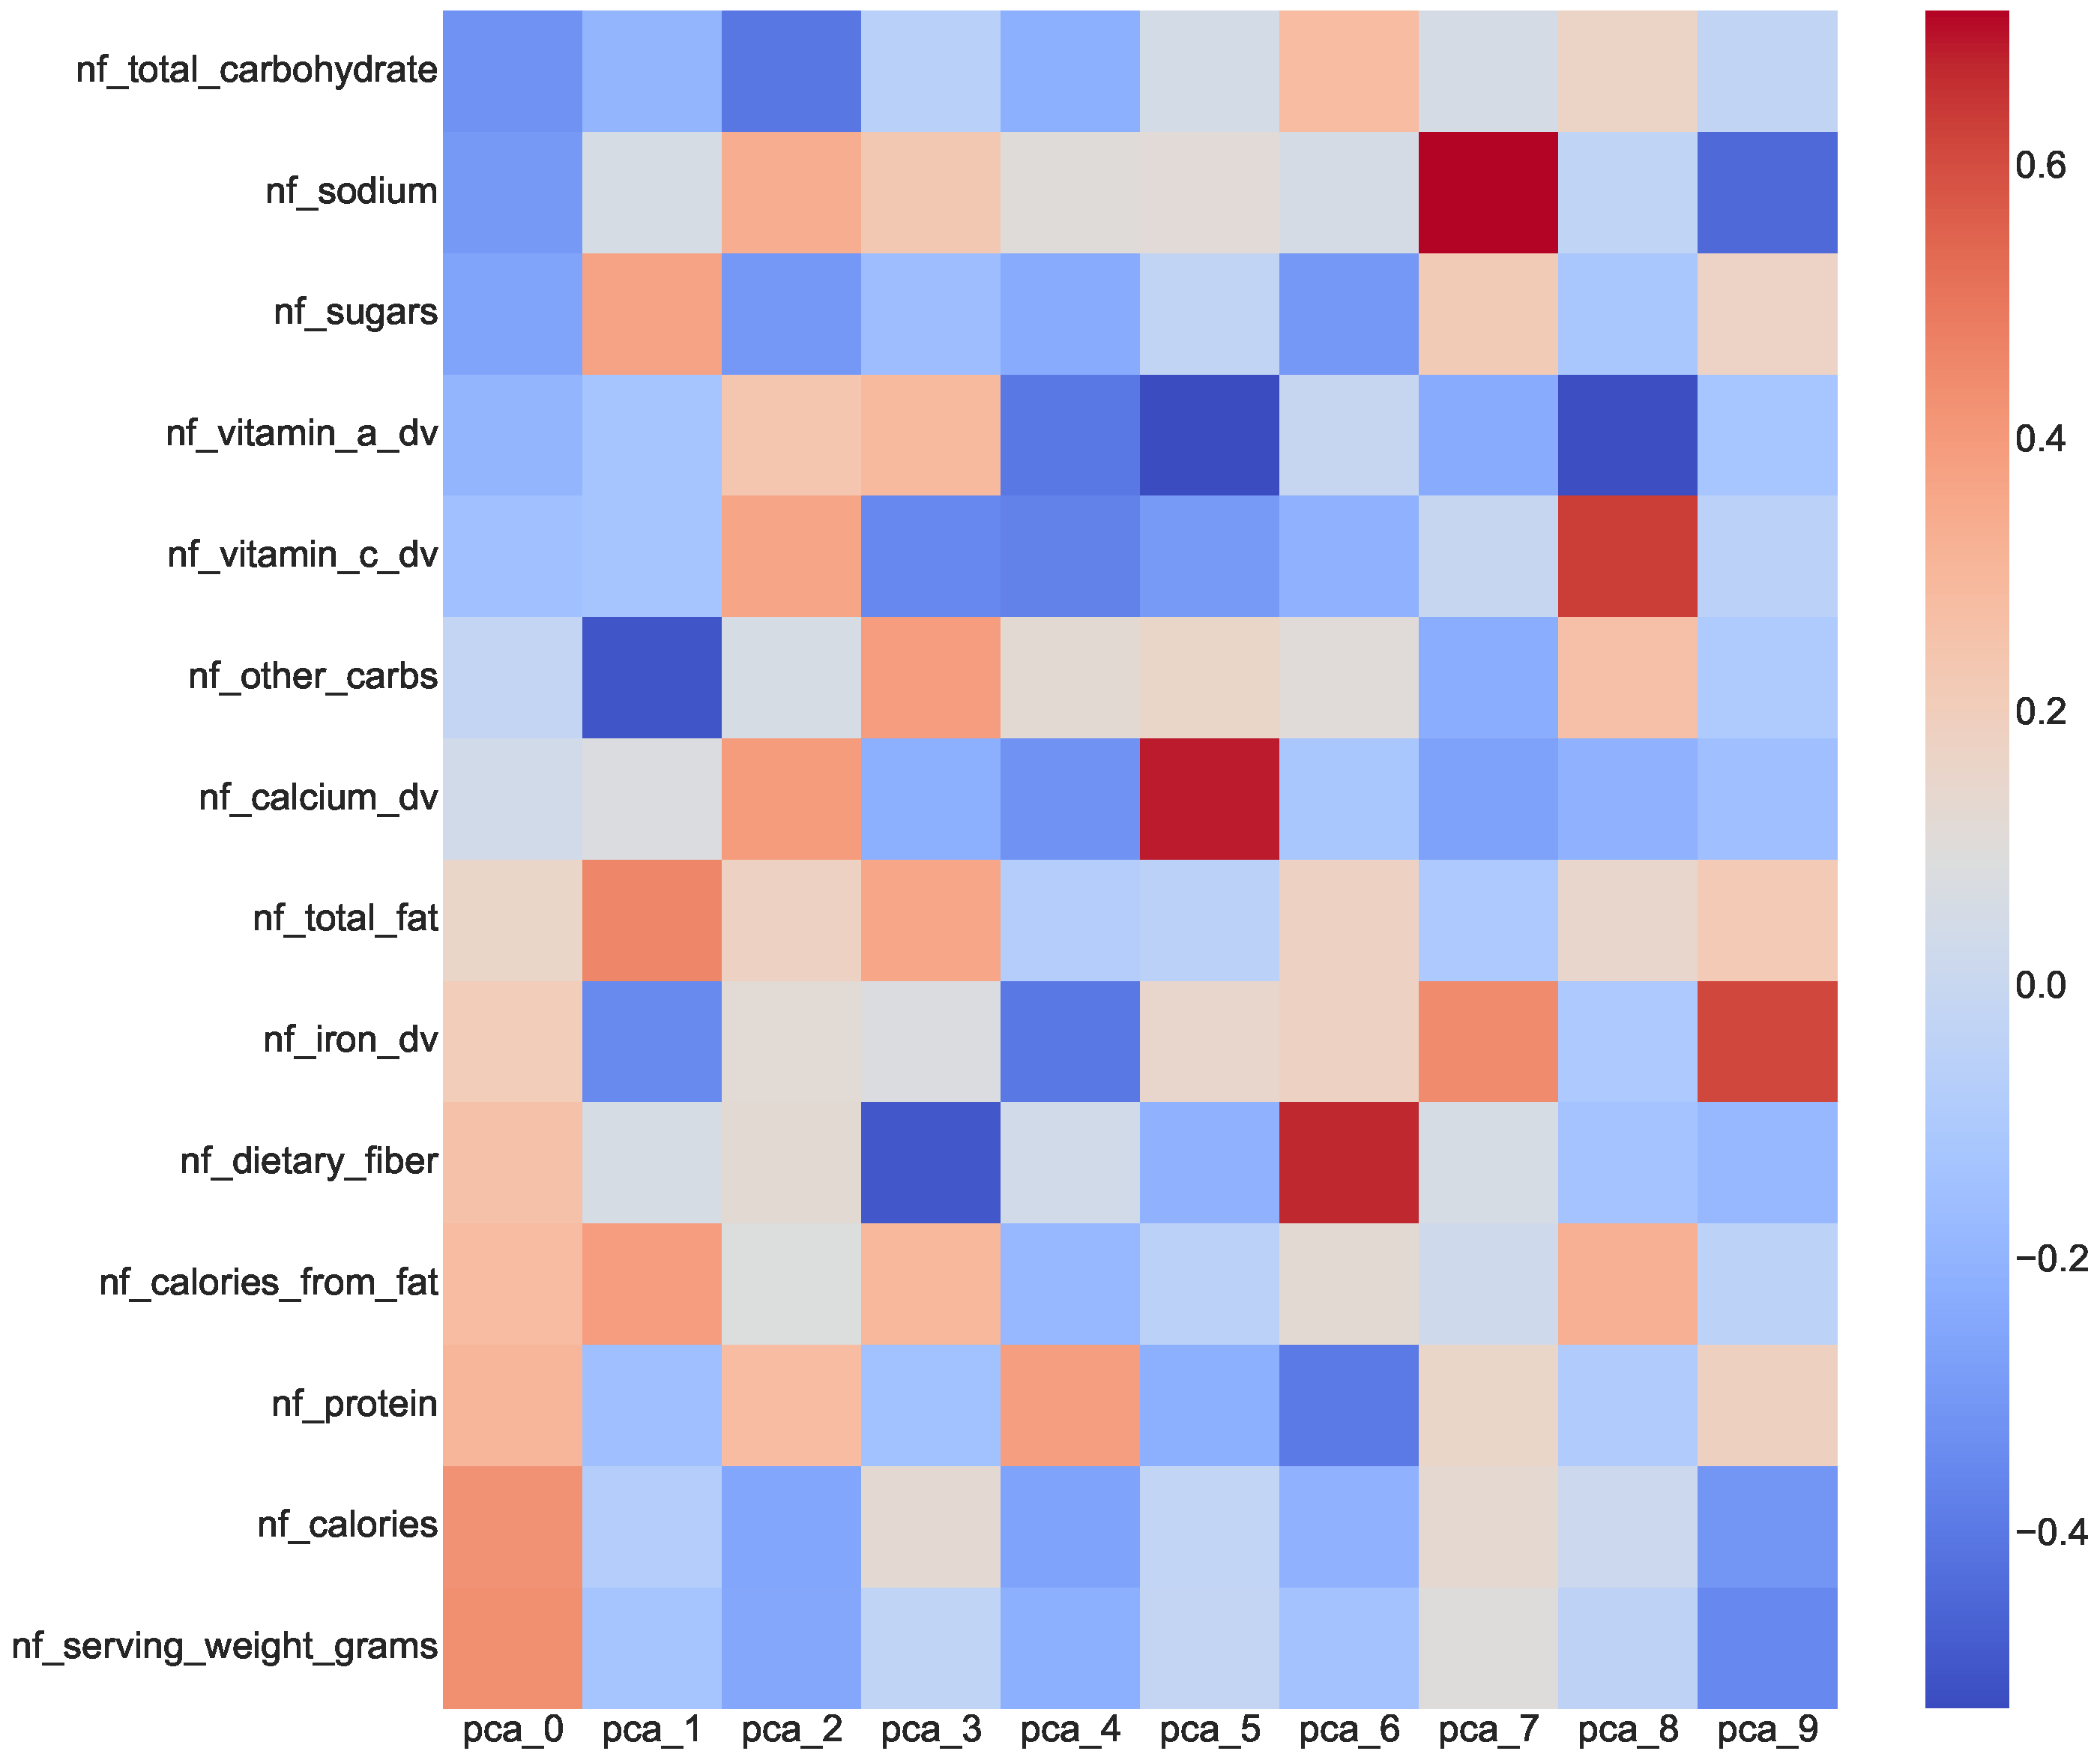
\includegraphics[height = \textheight ]{figures/pca_coeff.pdf}
\end{center}
\end{frame}


\begin{frame}[plain]
\begin{center}
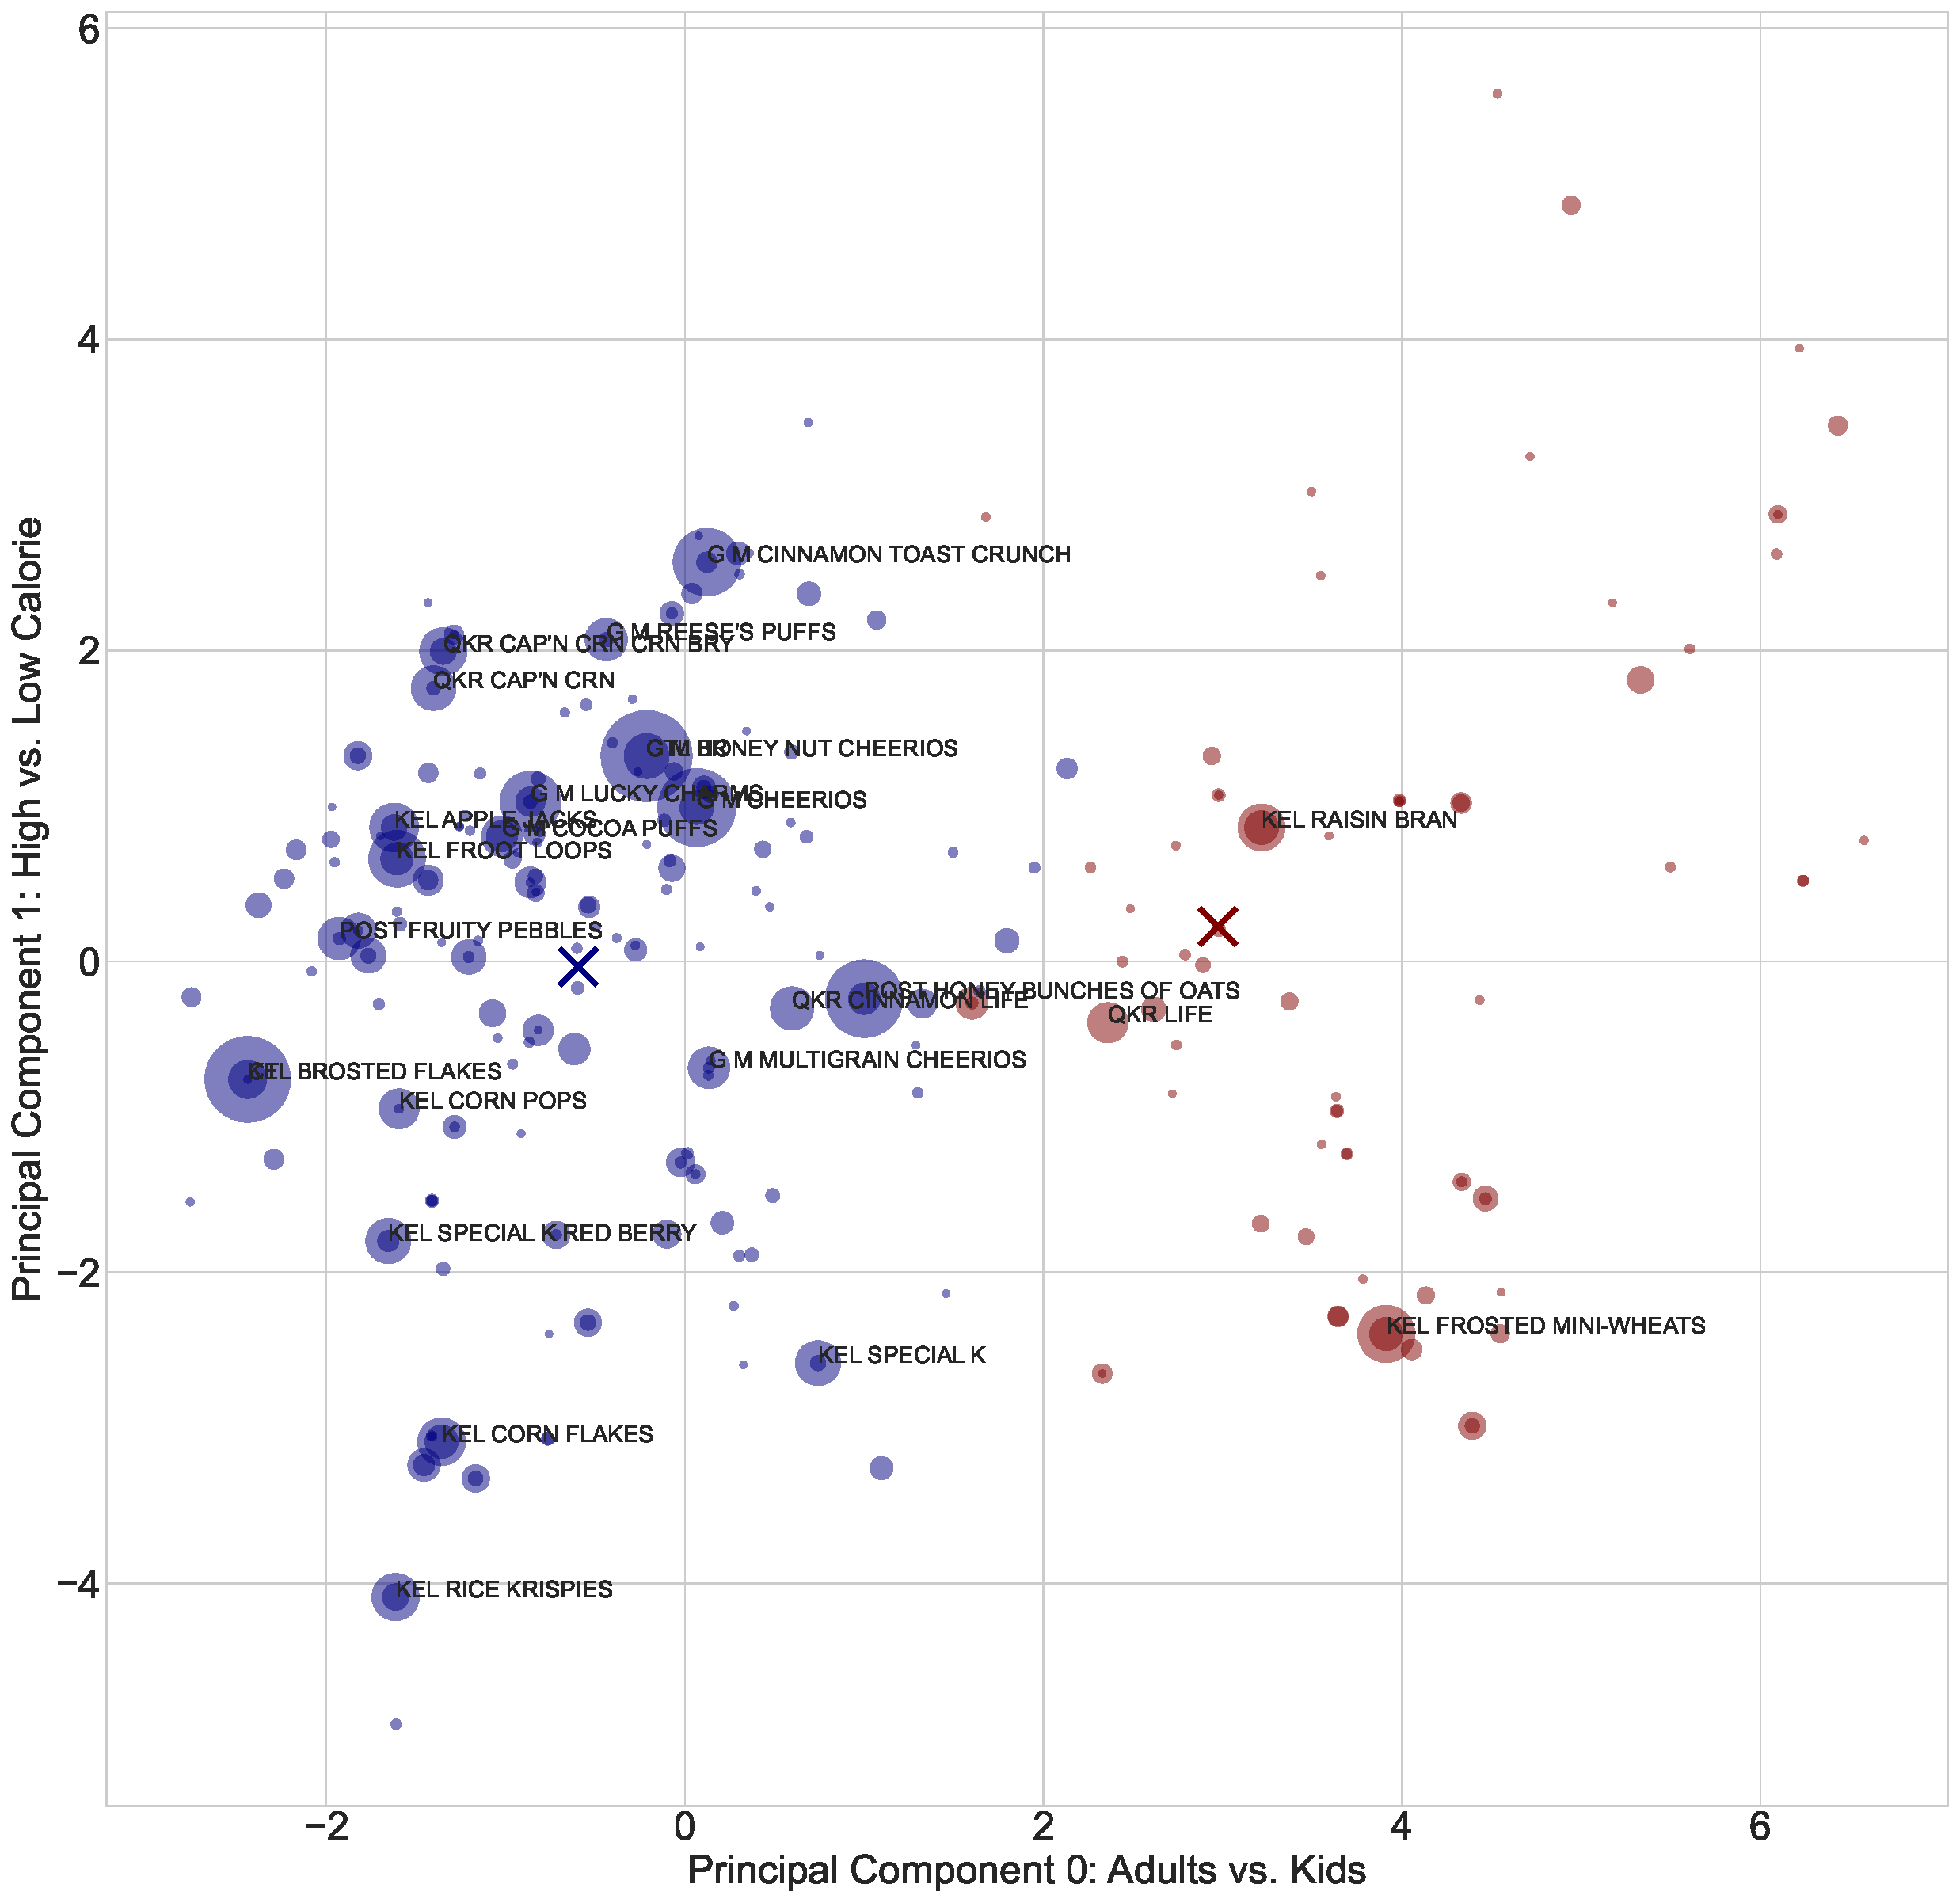
\includegraphics[height = \textheight ]{figures/pca_nests.pdf}
\end{center}
\end{frame}



\begin{frame}[plain,label=maindemand]{Demand Estimation}
\begin{itemize}
\item We estimate demand system using \texttt{PyBLP} (Conlon Gortmaker RJE 2020)
\item Highlights:
\begin{itemize}
\item We estimate market size from milk and egg purchases.
\item Observable demographic preference shocks (income and children).
\item Random coefficients on: (constant, price, branded, servings per box, 3 PC's)
\end{itemize}
\item Moments:
\begin{itemize}
\item Own input costs and local demographic variables.
\item ``Local'' Gandhi-Houde differentiation instruments
\item We convert these into 21 ``optimal instruments"
\item 520 micro-moments to get $\Pi$ and $\Sigma$.
\end{itemize}
\end{itemize}
\end{frame}


\begin{frame}{Implementation: Micro Moments}
Also have 520 ``micro-moments'' grouped by \texttt{DMA-Code/Retail Chain}
\begin{align*}
\mathbb{E} \left[x_{jt} \times y_{it} \mid \text{purchase } \right] 
- \mathbb{E}\left[x_{jt} \times y_{it}  \times \frac{s_{ijt}(\theta_1,\theta_2)}{1-s_{i0t}(\theta_1,\theta_2)}  \right] = 0.
\end{align*}
\begin{itemize}
\item Match observed interactions of characteristics (constant, price, branded, servings per box, PC) \& demographics from the model and the data.
\item Conditional on purchase.
\item We calculate these from Nielsen Panelist data by \texttt{chain-dma-year}.
\item We carefully track \# of observations to get variance calculations.
\item We bootstrap the covariance from the sample (but not model).
\end{itemize}
See Conlon Gortmaker (2022) for details.
\end{frame}

\begin{frame}{Parameters}
\begin{columns}
\begin{column}{0.4\textwidth}
\scalebox{0.33}{
\begin{tabular}{ll|c|cc|ccc} 
 \toprule 
 Parameter & Variable & \multicolumn{1}{c}{No $\Pi$ } & \multicolumn{2}{|c|}{No $\Sigma$ } & \multicolumn{3}{c}{Full Model} \\ 
 \midrule 
$\theta_2$ & & $\sigma^2$ & $\pi_{kids}$ & $\pi_{income}$ & $\pi_{kids}$ & $\pi_{income}$ & $\sigma^2$ \\ 
 \cmidrule(lr){1-1}\cmidrule{2-8} 
{} &          Constant &        40.102 &       3.837 &      0.333 &     2.505 &   -1.771 &    7.402 \\
{} &                   &         (1.136) &       (0.106) &      (0.080) &     (0.124) &    (0.076) &    (0.496) \\
{} &             Price &         8.263 &       0.676 &     -0.440 &     0.641 &   -0.715 &    0.415 \\
{} &                   &         (0.535) &       (0.027) &      (0.024) &     (0.034) &    (0.021) &    (0.035) \\
{} & Cov(Const, Price) &        18.203 &             &            &           &          &    1.750 \\
{} &                   &         (0.823) &             &            &           &          &    (0.128) \\
{} &             PCA\_0 &               &       0.061 &     -0.056 &     0.081 &   -0.028 &          \\
{} &                   &               &       (0.009) &      (0.005) &     (0.008) &    (0.005) &          \\
{} &             PCA\_1 &               &       0.084 &      0.011 &     0.077 &    0.007 &          \\
{} &                   &               &       (0.009) &      (0.005) &     (0.008) &    (0.006) &          \\
{} &             PCA\_2 &               &      -0.123 &      0.188 &    -0.090 &    0.074 &          \\
{} &                   &               &       (0.011) &      (0.006) &     (0.009) &    (0.006) &          \\
{} &           Branded &               &       0.043 &      0.158 &     0.807 &    0.582 &          \\
{} &                   &               &       (0.045) &      (0.037) &     (0.041) &    (0.041) &          \\
{} &      Servings/Box &               &      -0.048 &     -0.088 &    -0.036 &   -0.008 &          \\
{} &                   &               &       (0.004) &      (0.004) &     (0.004) &    (0.003) &          \\
\midrule 
 $\theta_1$ & & & & & & & \\ 
 \cmidrule(lr){1-1}\cmidrule{2-8} 
{} &            Price &\multicolumn{1}{c|}{3.143}&\multicolumn{2}{c|}{2.445}&\multicolumn{3}{c}{2.472} \\ 
{} &                  &\multicolumn{1}{c|}{(0.011)}&\multicolumn{2}{c|}{(0.025)}&\multicolumn{3}{c}{(0.027)} \\ 
{} &  Unemp x Branded &\multicolumn{1}{c|}{-0.043}&\multicolumn{2}{c|}{-0.016}&\multicolumn{3}{c}{-0.025} \\ 
{} &                  &\multicolumn{1}{c|}{(0.002)}&\multicolumn{2}{c|}{(0.002)}&\multicolumn{3}{c}{(0.002)} \\ 
{} &         Recall 1 &\multicolumn{1}{c|}{-0.259}&\multicolumn{2}{c|}{-0.299}&\multicolumn{3}{c}{-0.344} \\ 
{} &                  &\multicolumn{1}{c|}{(0.083)}&\multicolumn{2}{c|}{(0.073)}&\multicolumn{3}{c}{(0.075)} \\ 
{} &         Recall 2 &\multicolumn{1}{c|}{-0.215}&\multicolumn{2}{c|}{-0.154}&\multicolumn{3}{c}{-0.159} \\ 
{} &                  &\multicolumn{1}{c|}{(0.059)}&\multicolumn{2}{c|}{(0.054)}&\multicolumn{3}{c}{(0.056)} \\ 
{} &         Recall 3 &\multicolumn{1}{c|}{0.035}&\multicolumn{2}{c|}{0.05}&\multicolumn{3}{c}{0.058} \\ 
{} &                  &\multicolumn{1}{c|}{(0.074)}&\multicolumn{2}{c|}{(0.057)}&\multicolumn{3}{c}{(0.062)} \\ 
{} & log(Advertising) &\multicolumn{1}{c|}{0.03}&\multicolumn{2}{c|}{0.03}&\multicolumn{3}{c}{0.03} \\ 
{} &                  &\multicolumn{1}{c|}{(0.002)}&\multicolumn{2}{c|}{(0.002)}&\multicolumn{3}{c}{(0.002)} \\ 
\midrule 
 \multicolumn{2}{l|}{Model Predictions} &  50\% & \multicolumn{2}{c|}{50\%} & 25\% & 50\% & 75\%  \\ 
 \midrule 
 & Own Elasticity           & -2.923 &\multicolumn{2}{c|}{ -2.676 }& -3.055 & -2.812 & -2.592 \\
 & Aggregate Elasticity     & -0.351 &\multicolumn{2}{c|}{ -0.402 }& -0.435 & -0.393 & -0.348 \\
& Outside Good Diversion    &  0.384 &\multicolumn{2}{c|}{  0.570 }&  0.425 &  0.499 &  0.574 \\
\cmidrule{2-8}  
& Lerner (Own Profit Max)   &  0.307 &\multicolumn{2}{c|}{  0.411 }&  0.351 &  0.394 &  0.446 \\
& Lerner (Common Ownership) &  0.351 &\multicolumn{2}{c|}{  0.446 }&  0.372 &  0.428 &  0.501 \\
& Lerner (Big Four)         &  0.444 &\multicolumn{2}{c|}{  0.512 }&  0.408 &  0.497 &  0.621 \\
& Lerner (Monopoly)         &  0.713 &\multicolumn{2}{c|}{  0.648 }&  0.531 &  0.676 &  0.885 \\
\bottomrule 
\end{tabular}
}
\end{column}
\begin{column}{0.6\textwidth}
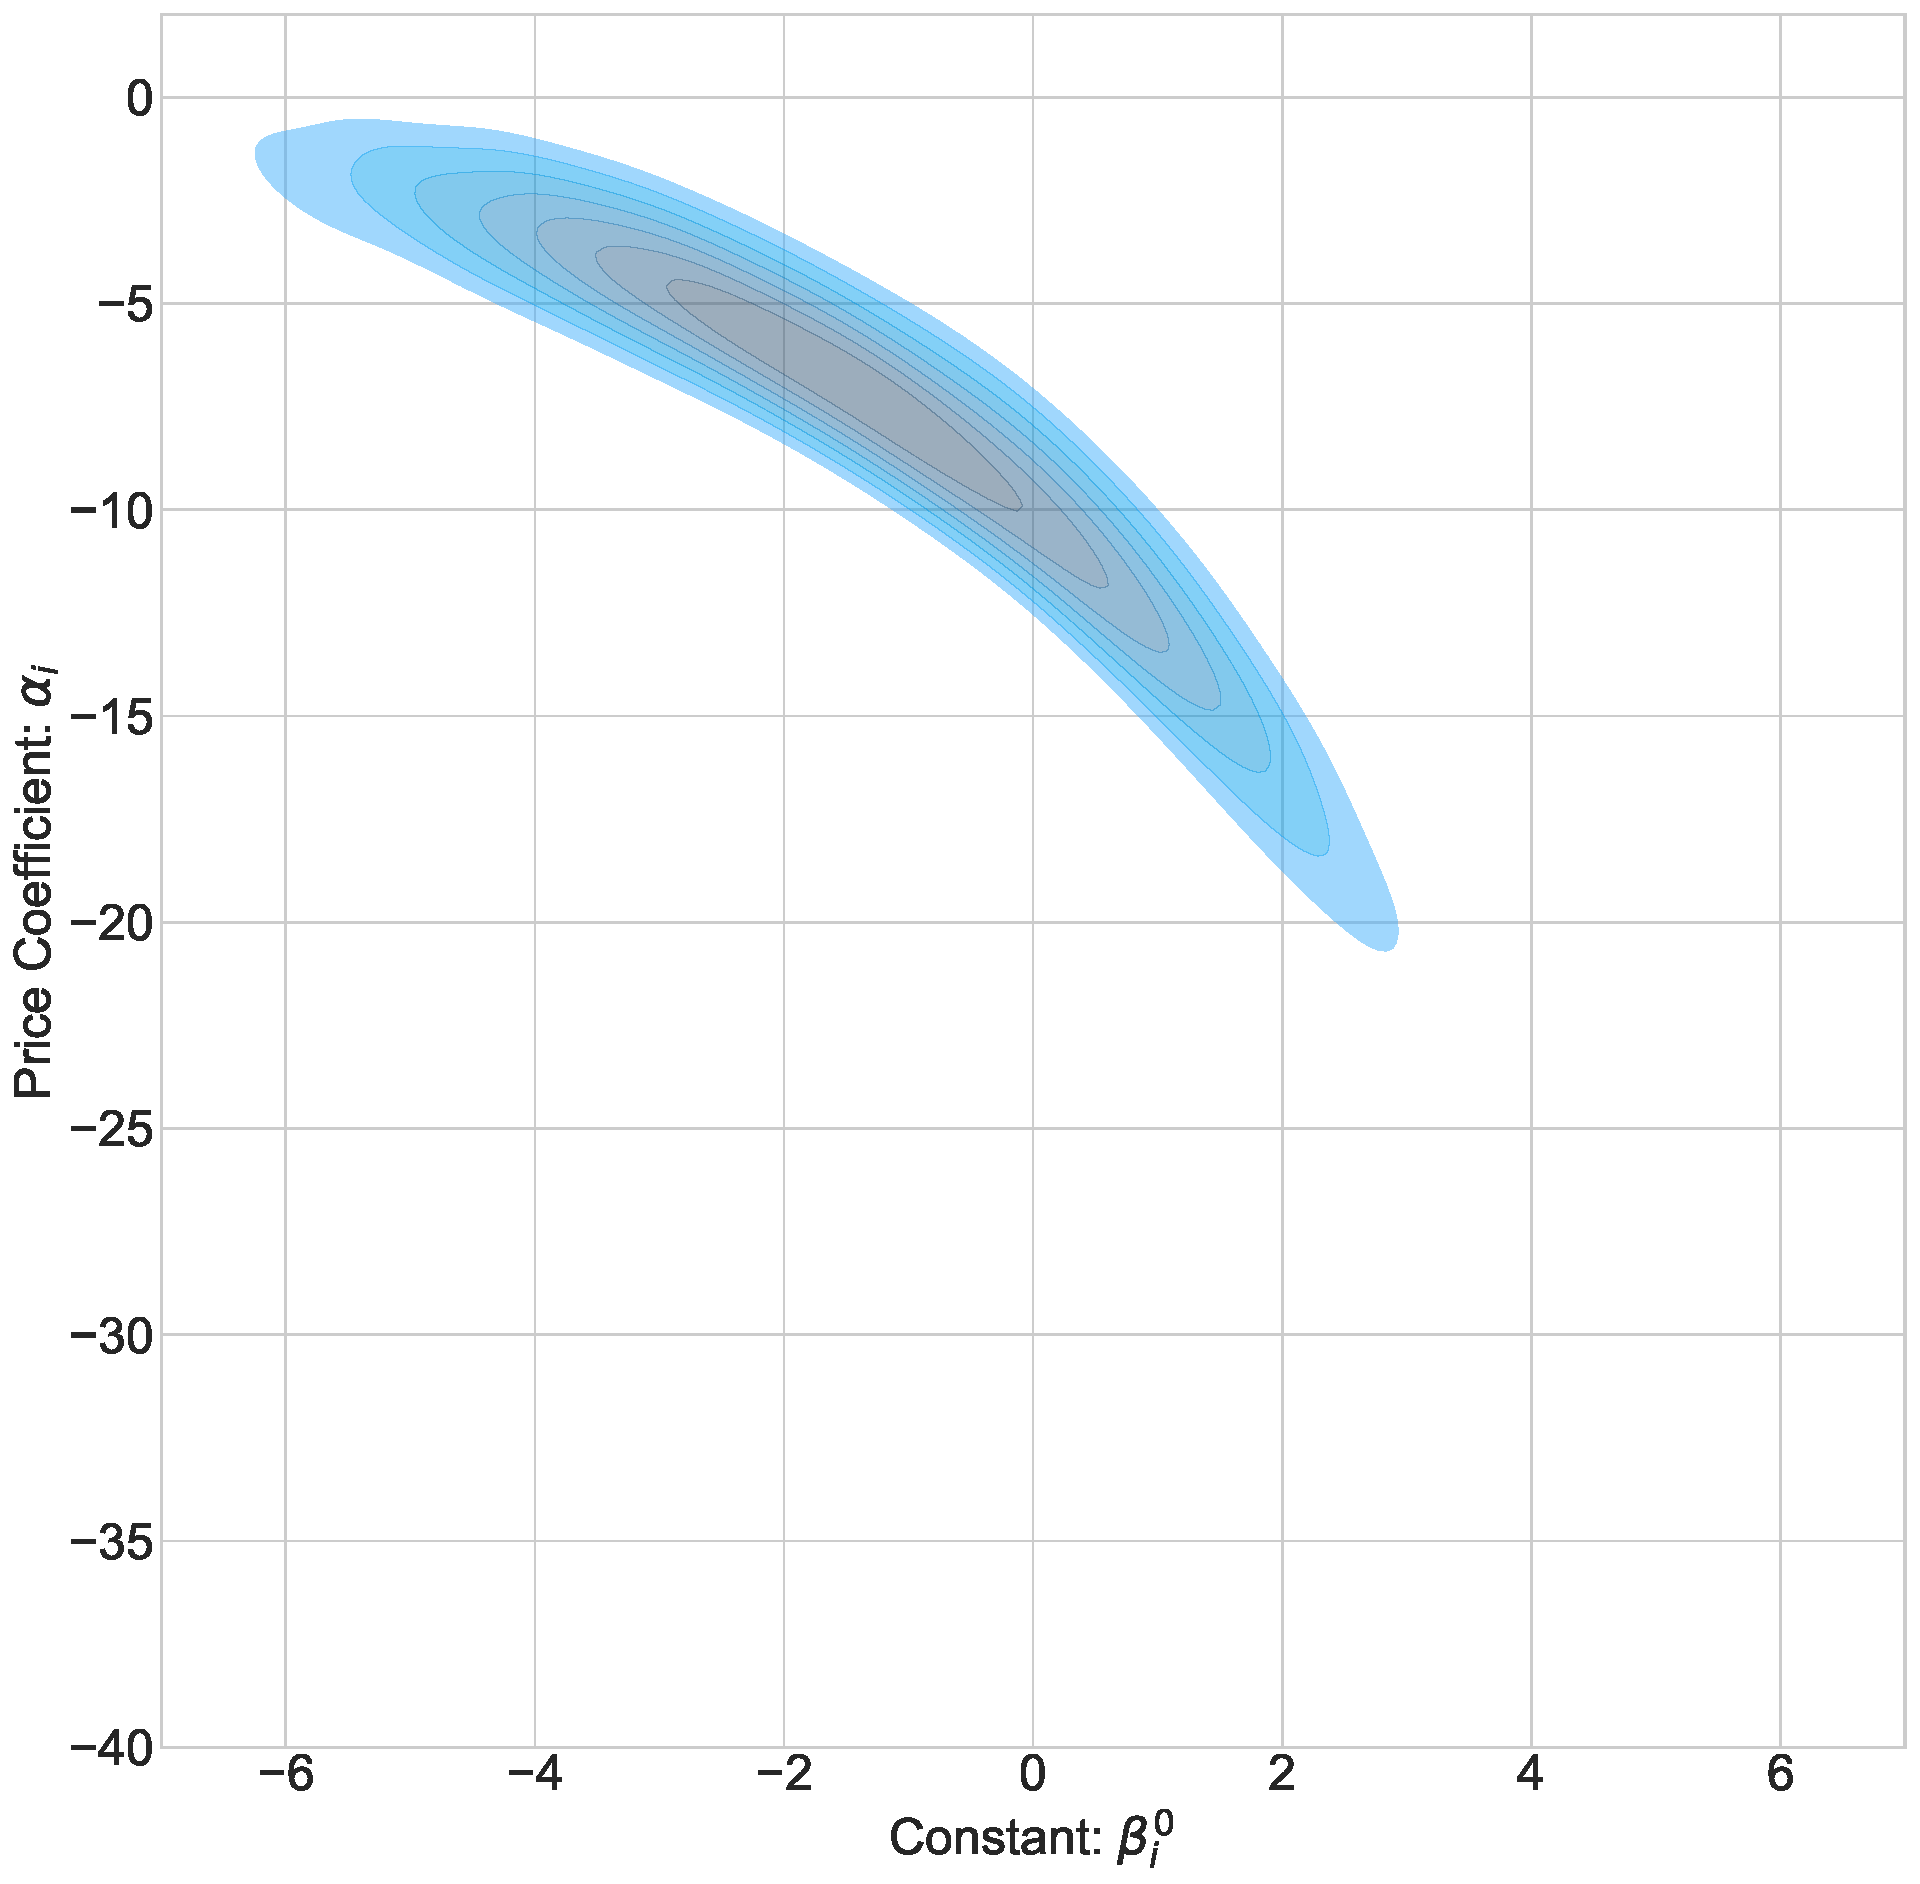
\includegraphics[width=0.9\textwidth]{resources/2d_density_plot.pdf}
\end{column}
\end{columns}
\end{frame}



\begin{frame}{Diversion Ratios}
\begin{align*}
D_{jk} = \frac{\partial q_j}{\partial p_k}/\left|\frac{\partial q_j}{\partial p_j}\right| = \frac{e_{jk}}{e_{jj}} \cdot \frac{q_j}{q_k}
\end{align*}
\begin{itemize}
  \item Easier to interpret than cross elasticity
  \item Higher diversion implies closer competition
  \item See Conlon Mortimer (RJE 2021) for all kinds of tricks.
\end{itemize}
\end{frame}
\begin{frame}[plain]
\begin{center}
\scalebox{0.6}{
\begin{tabular}{lrrrrrrr}
\toprule
{} &  Cheerios &  Special K &  Corn Flakes &  Reese's Puffs &  Capt Crunch &  Froot Loops &  Shares \\
\midrule
HN Cheerios         &      5.07 &       4.27 &         3.75 &           5.33 &         3.58 &         3.48 &    2.69 \\
Frosted Flakes      &      2.46 &       2.54 &         4.54 &           4.00 &         5.35 &         7.24 &    2.65 \\
Cheerios            &     - &       5.91 &         3.13 &           3.19 &         1.36 &         1.77 &    2.10 \\
Honey Bunches       &      2.47 &       2.51 &         2.21 &           2.08 &         1.94 &         1.99 &    1.47 \\
Cinn Toast Crunch   &      3.43 &       2.10 &         1.69 &           3.00 &         1.78 &         1.84 &    1.43 \\
Froot Loops         &      1.26 &       1.19 &         1.64 &           1.69 &         1.82 &        - &    1.18 \\
Lucky Charms        &      2.18 &       1.64 &         1.57 &           2.99 &         1.59 &         1.58 &    1.14 \\
Frosted Mini-Wheats &      0.36 &       0.50 &         0.74 &           0.68 &         0.87 &         1.27 &    1.01 \\
Corn Flakes         &      2.01 &       2.18 &        - &           1.31 &         1.24 &         1.52 &    0.98 \\
Rice Krispies       &      1.50 &       1.72 &         1.56 &           0.89 &         0.68 &         1.25 &    0.96 \\
Apple Jacks         &      0.91 &       0.80 &         1.24 &           1.27 &         1.42 &         2.45 &    0.85 \\
Raisin Bran (KEL)   &      0.46 &       0.47 &         0.63 &           0.78 &         0.82 &         1.24 &    0.79 \\
Special K Red Berry &      0.96 &       1.45 &         0.95 &           0.78 &         0.68 &         0.90 &    0.75 \\
Special K           &      2.06 &      - &         1.18 &           0.71 &         0.44 &         0.58 &    0.74 \\
MG Cheerios         &      1.11 &       0.99 &         0.75 &           0.89 &         0.54 &         0.66 &    0.71 \\
Reese's Puffs       &      1.36 &       0.86 &         0.87 &          - &         1.08 &         1.01 &    0.69 \\
Life                &      1.15 &       1.12 &         1.05 &           1.02 &         1.72 &         0.89 &    0.68 \\
Cocoa Puffs         &      1.18 &       0.92 &         0.95 &           1.47 &         1.05 &         0.97 &    0.67 \\
Capt Crunch         &      0.63 &       0.58 &         0.88 &           1.21 &        - &         1.19 &    0.62 \\
Capt Crunch Berry   &      0.68 &       0.61 &         0.83 &           1.15 &         3.29 &         1.00 &    0.58 \\
Corn Pops           &      0.43 &       0.43 &         0.71 &           0.66 &         0.75 &         1.45 &    0.56 \\
Cinn Life           &      0.76 &       0.75 &         0.83 &           0.84 &         1.59 &         0.78 &    0.54 \\
Fruity Pebbles      &      0.61 &       0.59 &         0.71 &           0.71 &         0.75 &         0.77 &    0.44 \\
\midrule
Own Elas            &      -2.46&       -2.66 &       -2.64 &           -2.70 &        -2.68 &       -2.71 &  - \\
\bottomrule
\end{tabular}
}
\end{center}
\end{frame}


\begin{frame}[plain]{Single Product: Implied Marginal Costs}
\begin{center}
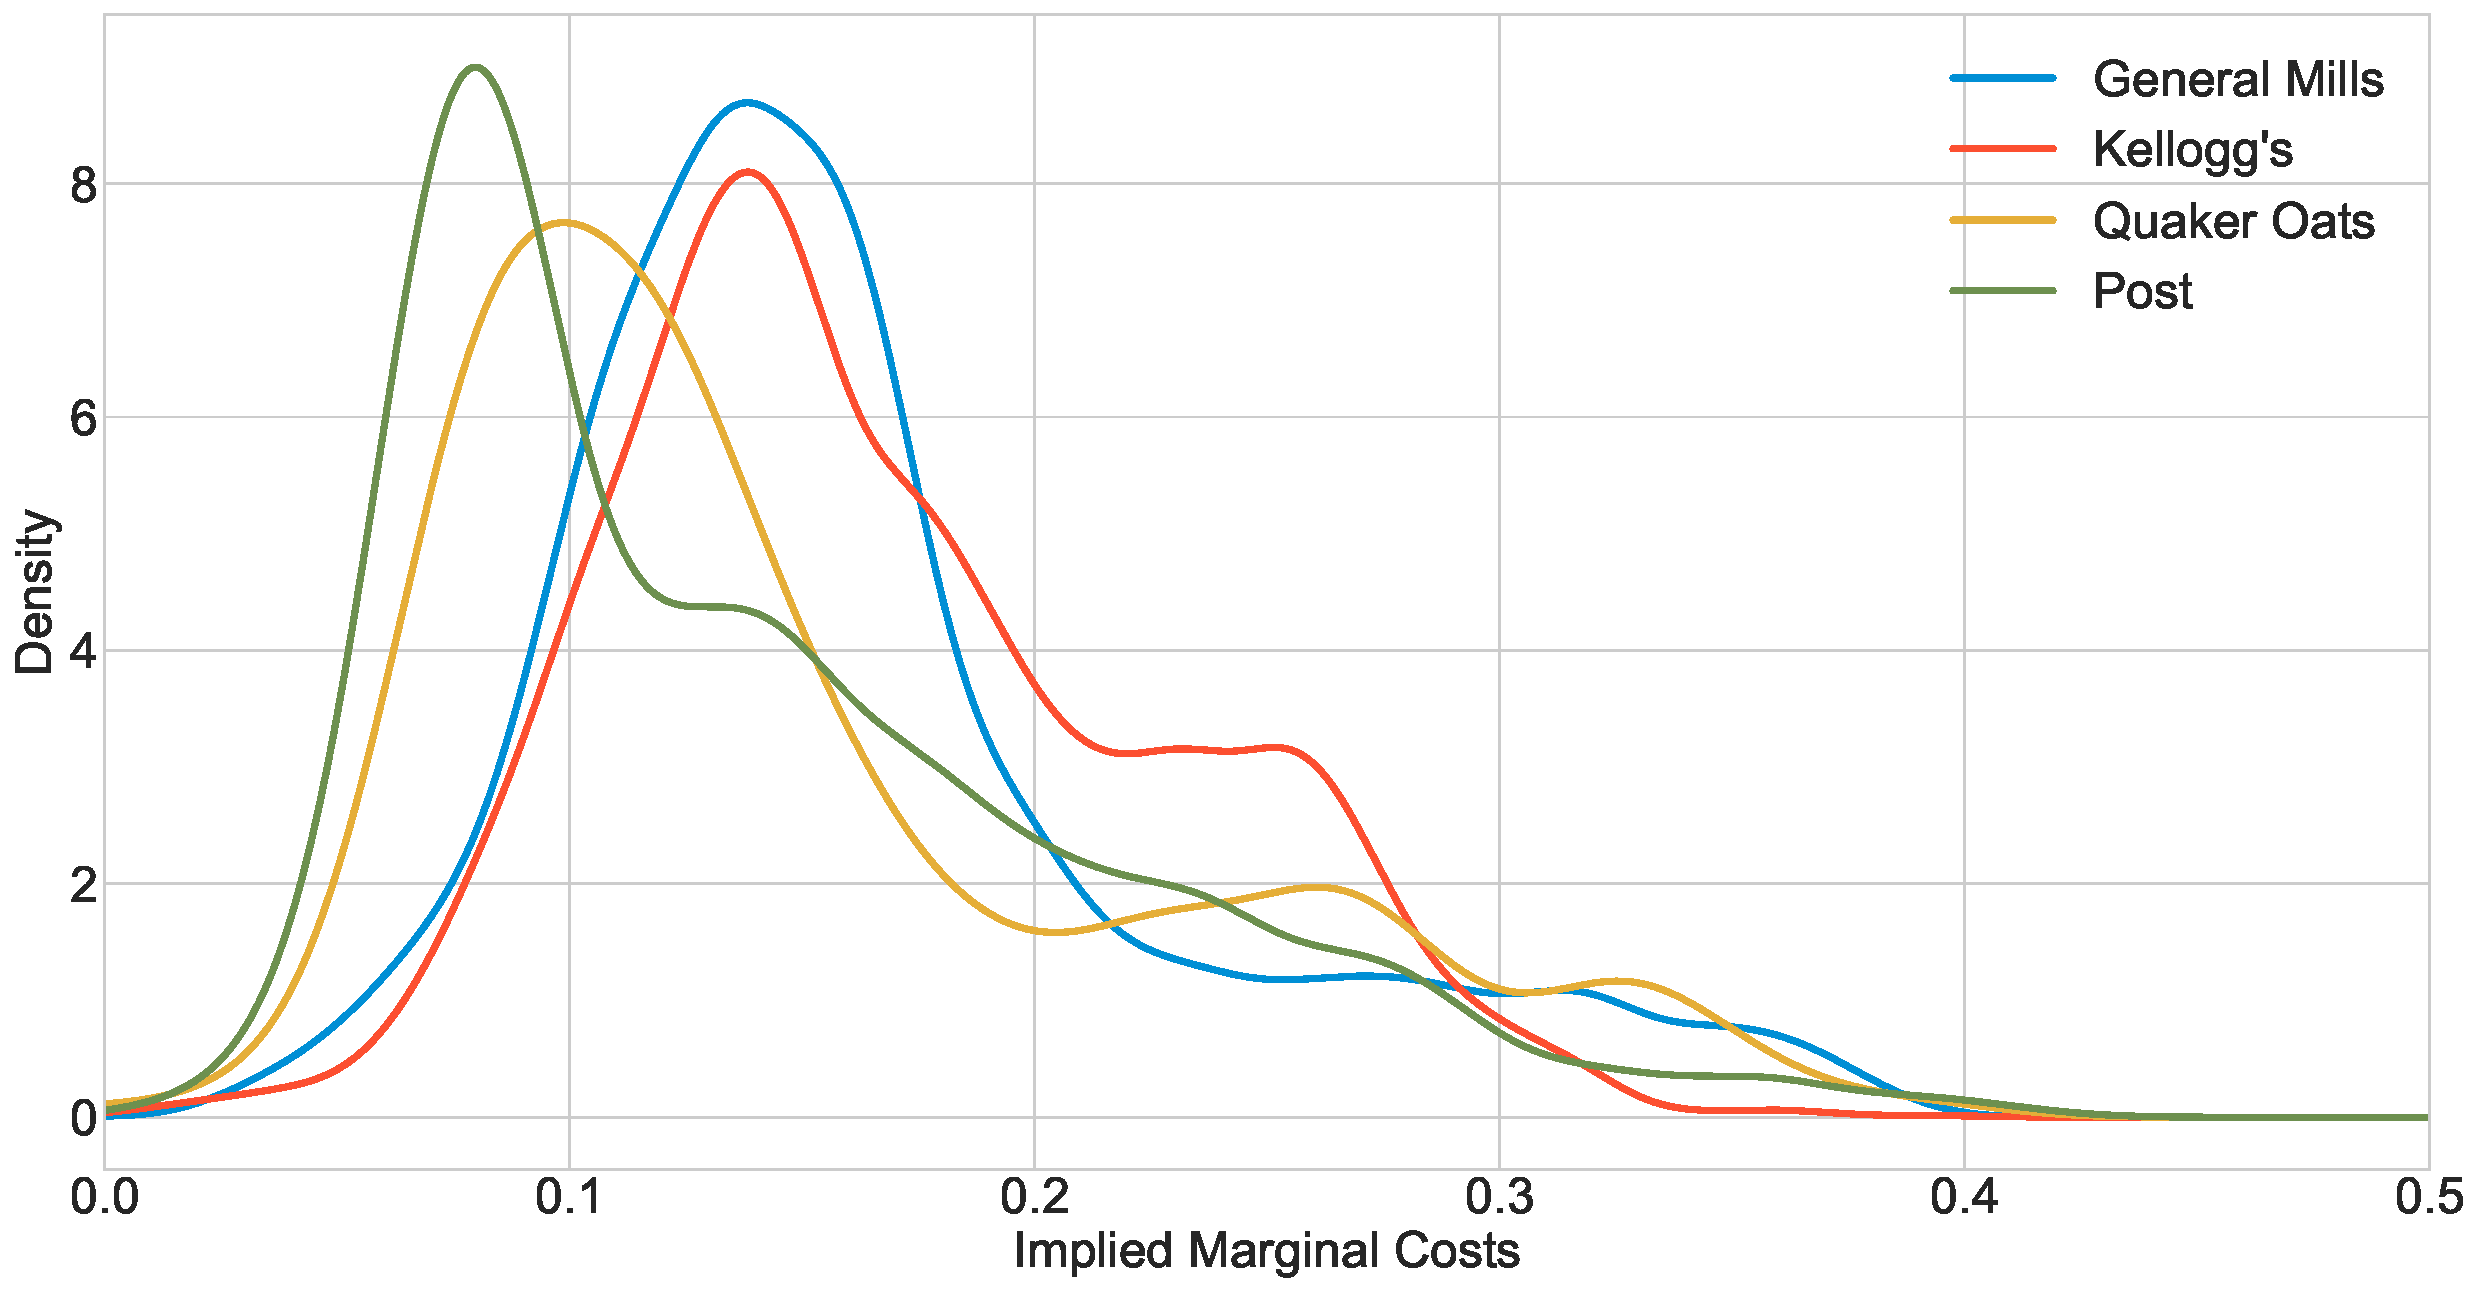
\includegraphics[height =0.8\textheight]{figures/mu_all_bertrand_real.pdf}
\end{center}
\end{frame}



\begin{frame}[plain]{Predicted Markups (Q4 2016)}
\begin{center}
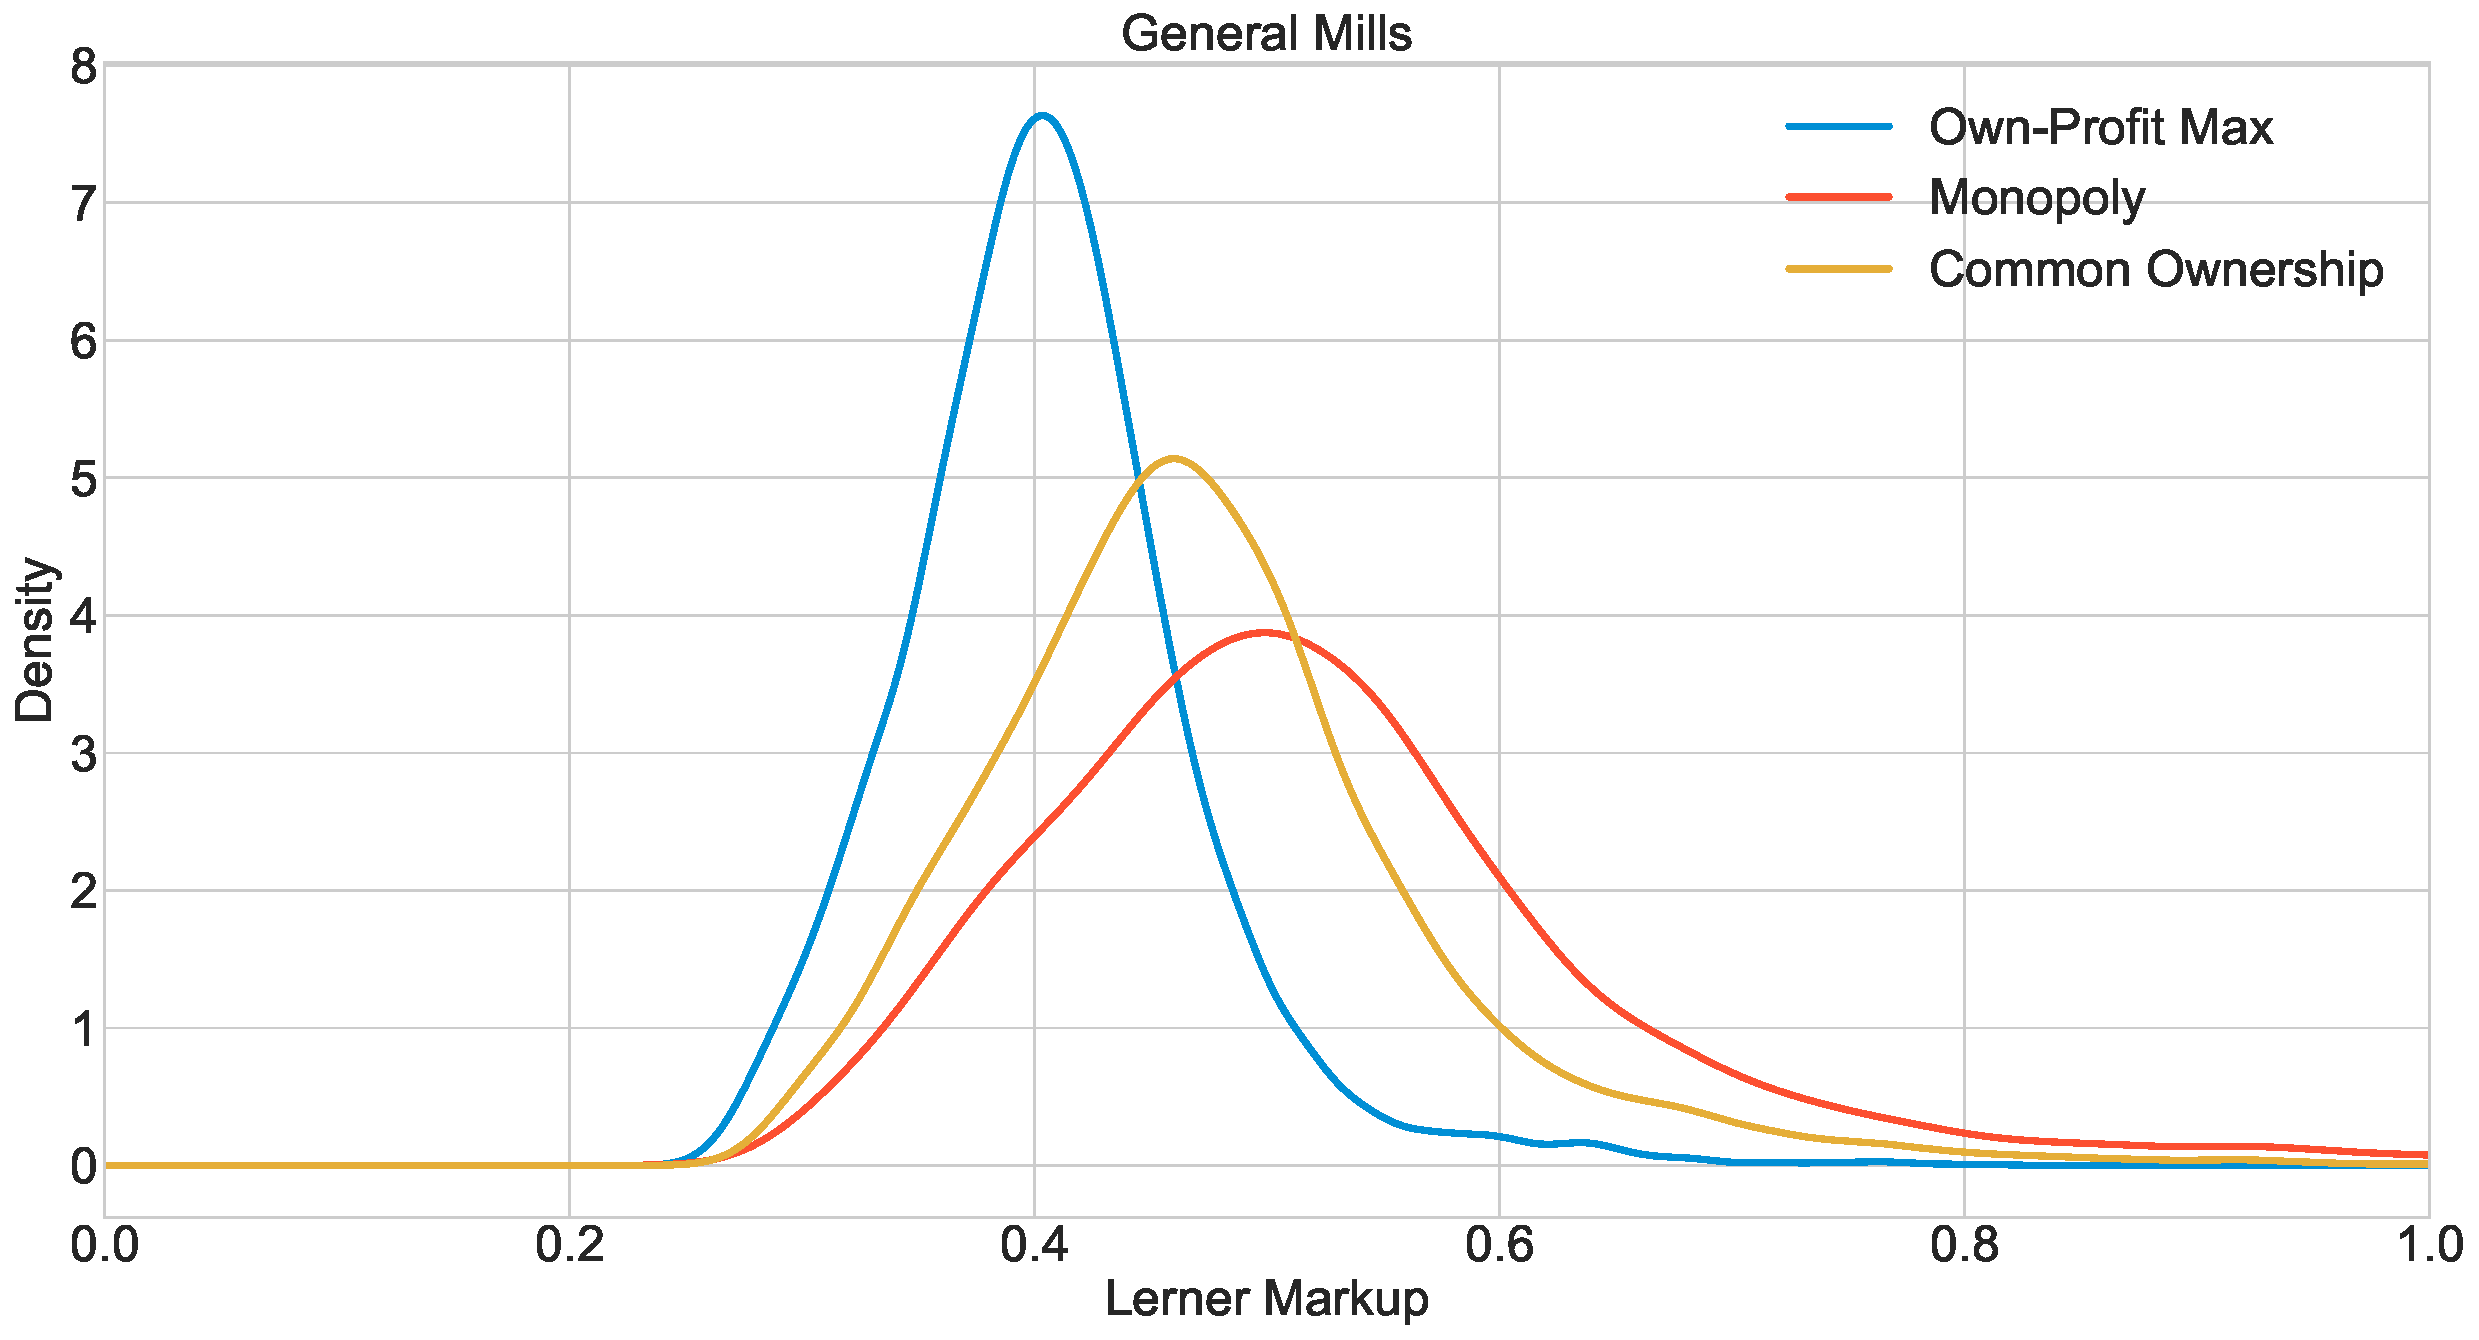
\includegraphics[width = 6.5cm]{figures/mu_gm_real.pdf}
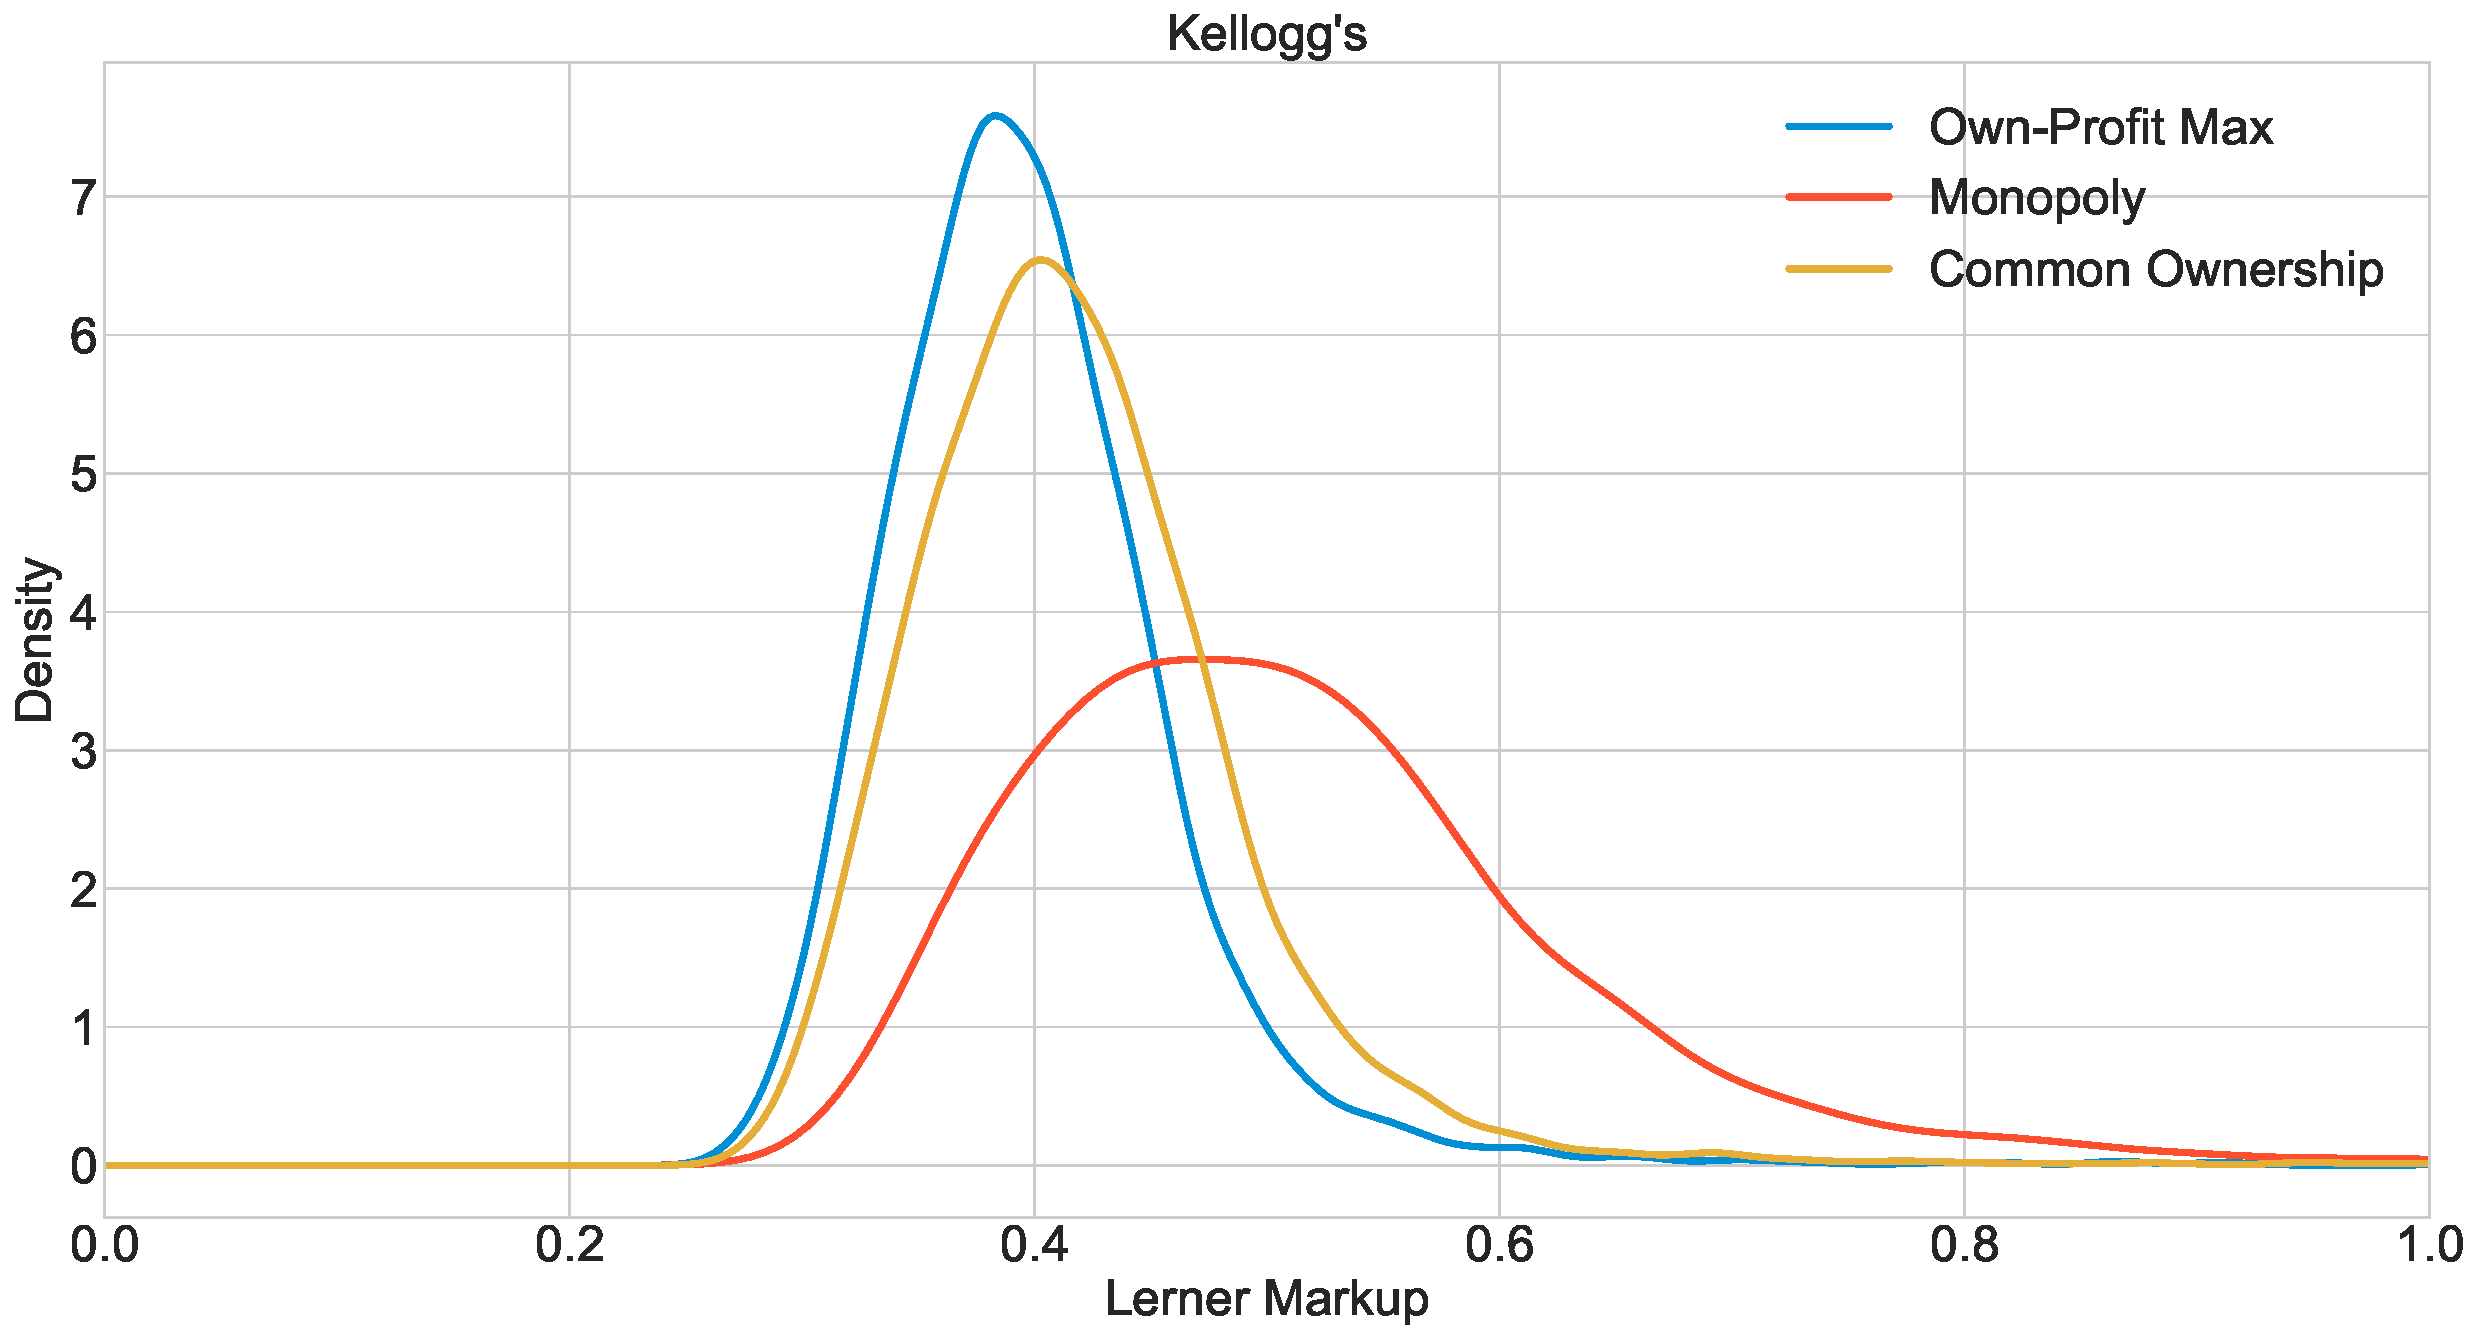
\includegraphics[width = 6.5cm]{figures/mu_kel_real.pdf}\\
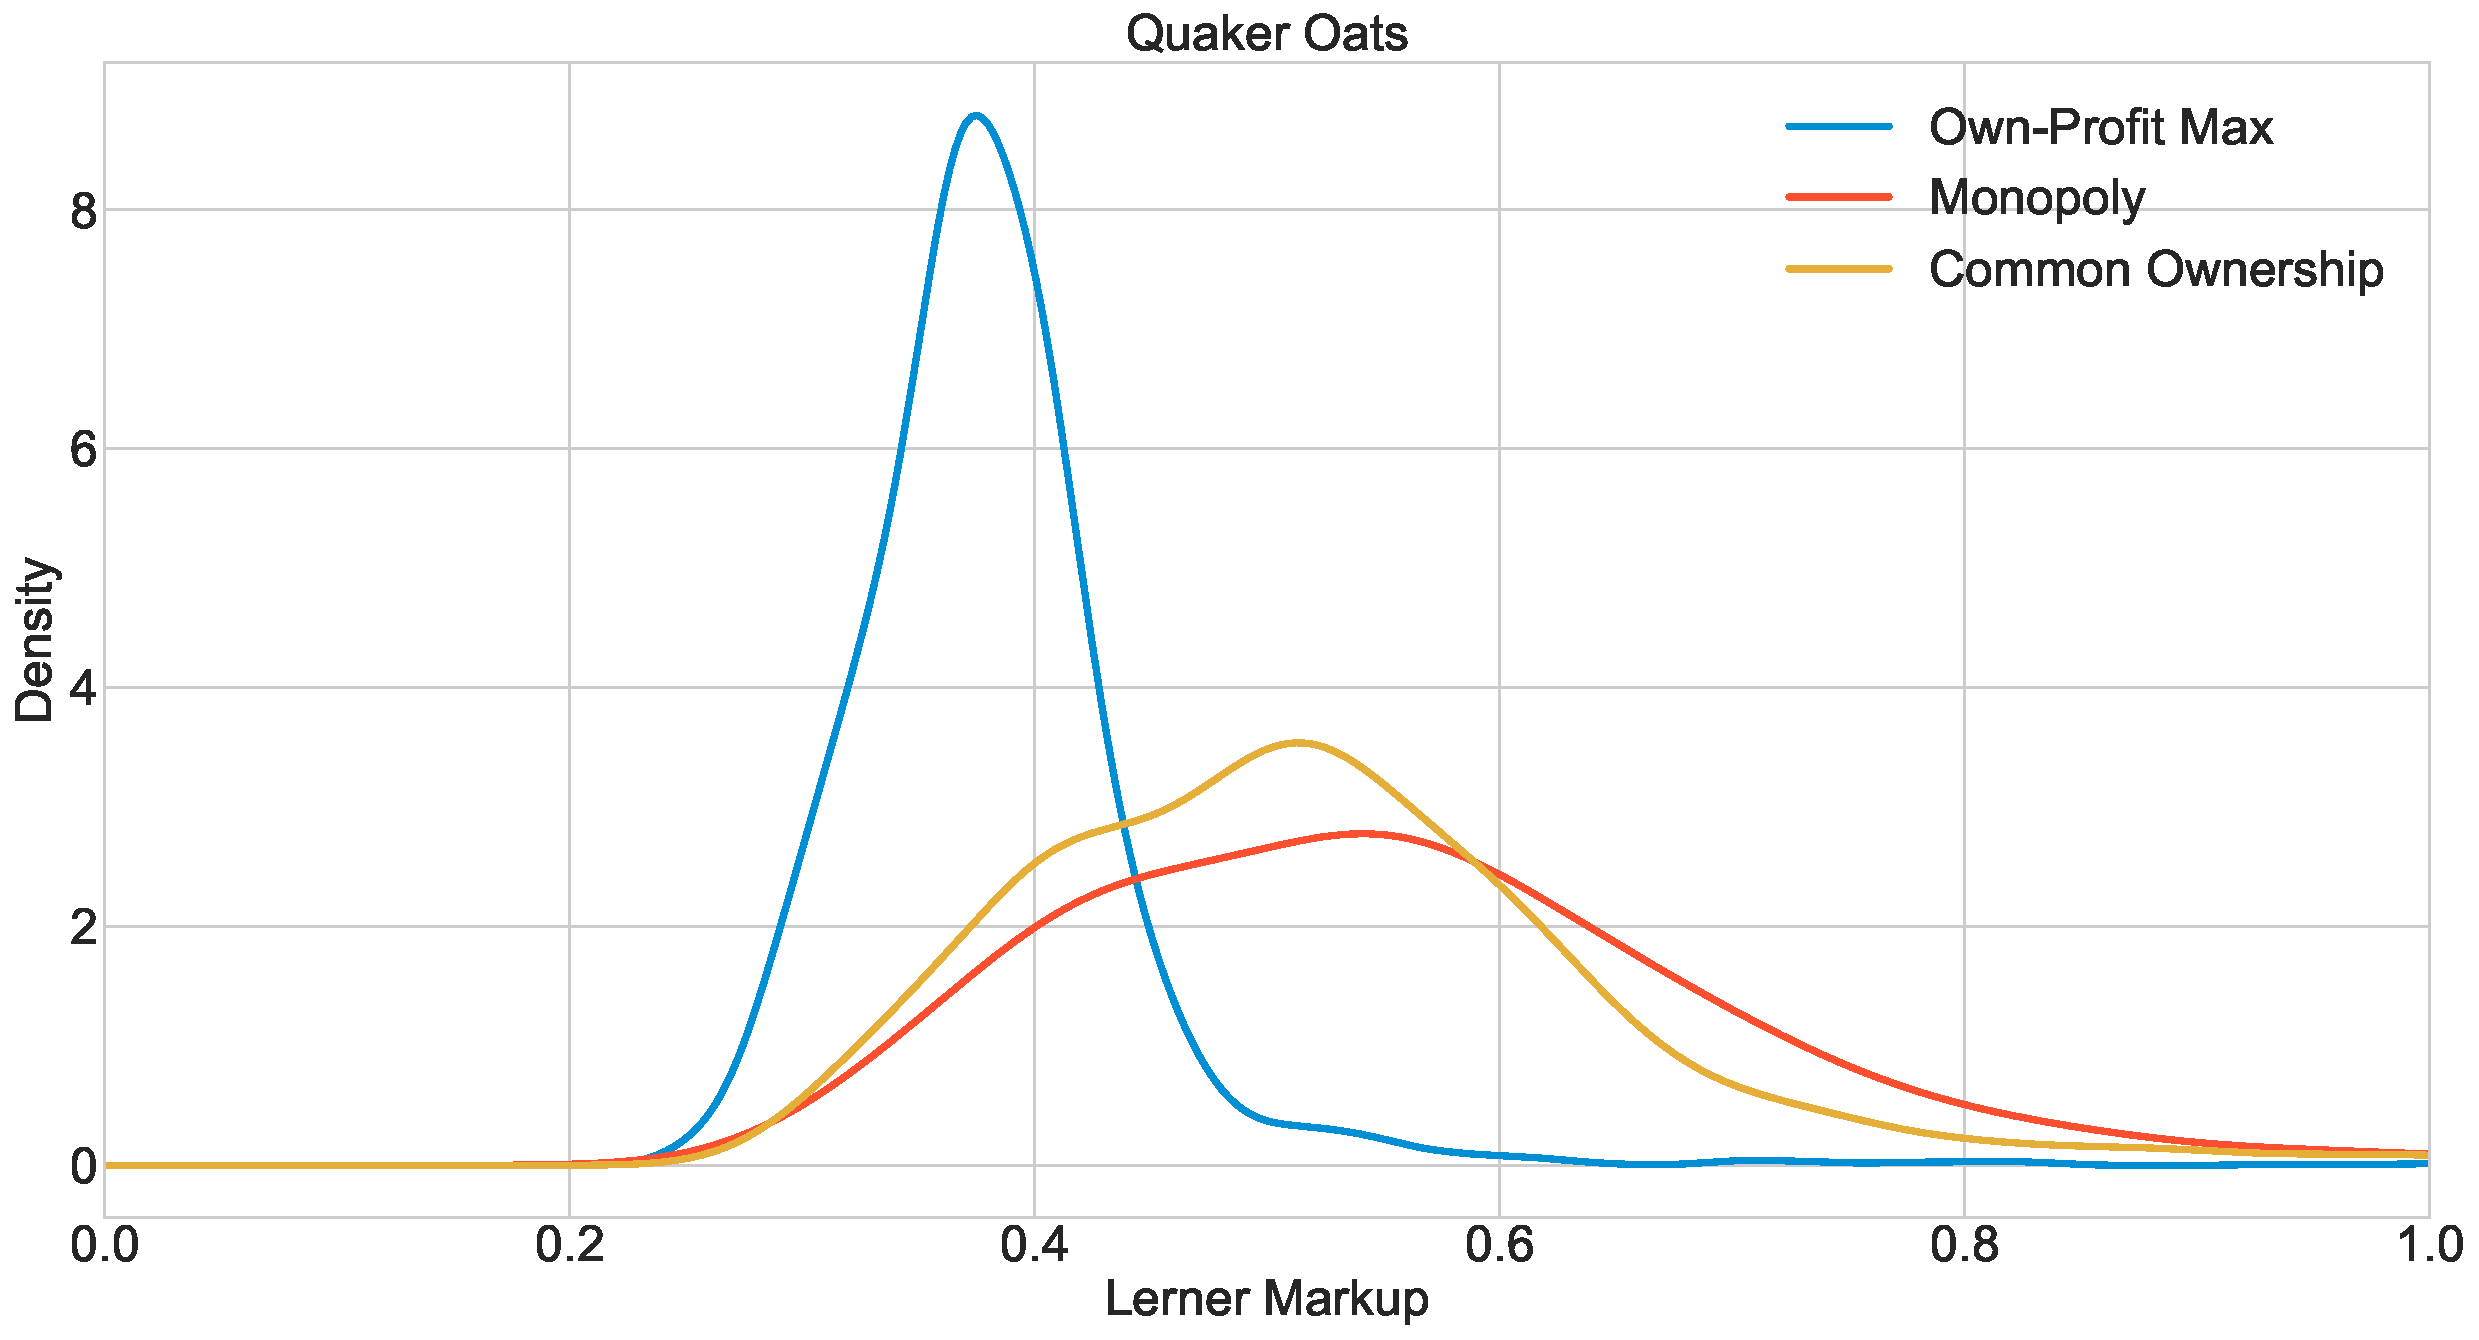
\includegraphics[width = 6.5cm]{figures/mu_qkr_real.pdf}
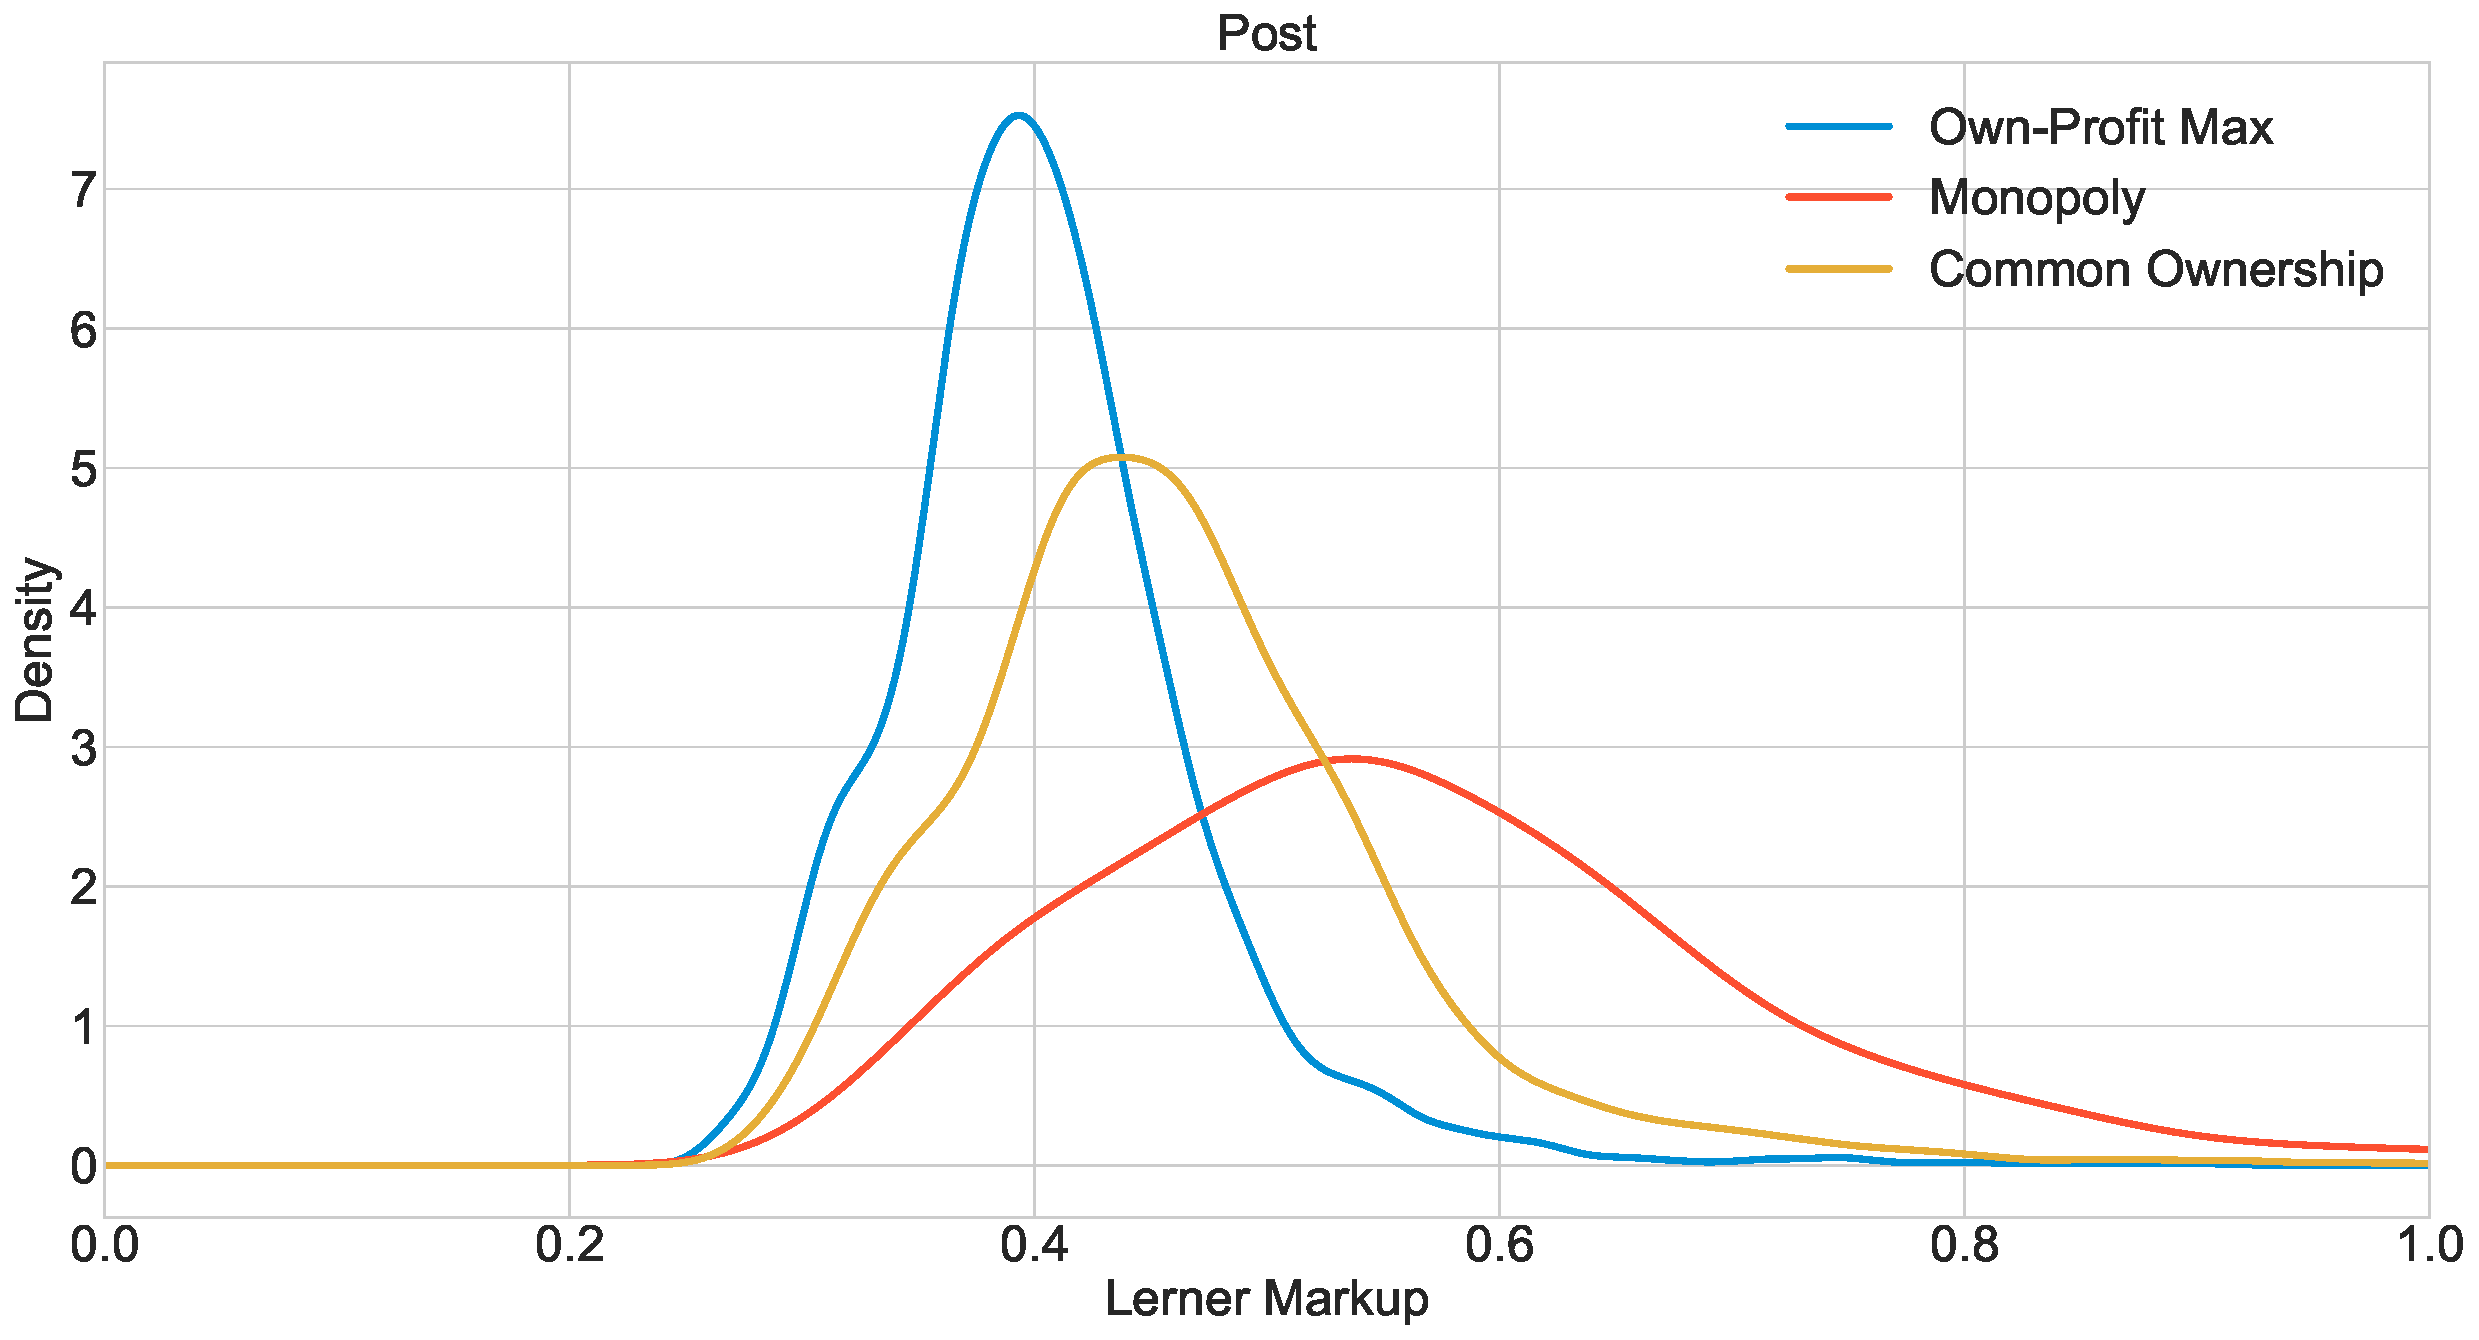
\includegraphics[width = 6.5cm]{figures/mu_post_real.pdf}
\end{center}
\end{frame}


\begin{frame}[plain, label=merger]{Counterfactual Price Increases}
\begin{center}
\scalebox{0.75}{
\begin{tabular}{lrrrrrrrr}
\toprule
{} &  GM-KEL &  GM-QKR &  GM-POST &  KEL-QKR &  KEL-POST &  QKR-POST &  Monopoly &  $\kappa^{CO}$ \\
\midrule
GIS     &    6.94 &    1.53 &     3.30 &    -0.03 &     -0.09 &     -0.05 &     12.22 &           4.81 \\
K       &    6.69 &   -0.03 &    -0.06 &     1.46 &      3.43 &     -0.03 &     12.07 &           6.87 \\
PEP     &   -0.21 &    8.86 &    -0.22 &     8.72 &     -0.22 &      4.48 &     22.41 &          10.67 \\
POST    &   -0.10 &   -0.08 &     7.43 &    -0.09 &      7.98 &      1.75 &     17.49 &           8.49 \\
Overall &    4.49 &    1.10 &     2.25 &     1.08 &      2.40 &      0.57 &     12.50 &           6.01 \\
\bottomrule
\end{tabular}

}
\end{center}
\vspace{1cm}
NB: Computed using marginal costs as predicted by own-profit maximization.\\
Greater than pairwise mergers, 48\% of way to monopoly.\\
Private label provides a LOT of discipline.\\
Strategic substitutes: Negative correlation of $(\beta_{i0}, \alpha_{i})$
\end{frame}


\begin{frame}[plain,label=mainresults]{Main Results: These are $N(0,1)$}
\begin{center}
\scalebox{0.5}{\begin{tabularx}{500pt}{l*4             {>{\Centering}X}}\toprule
{} &  Others' Cost &  Demographics &  BLP Inst. &  Dmd. Opt. Inst. \\
\midrule \multicolumn{1}{c}{Own Profit Max vs.}&             \multicolumn{4}{c}{Panel 1: $A(\mathbf{z}_t)=\mathbf{z}_t,$ linear $h_s(\cdot)$ }\\                 \cmidrule(lr){1-1} \cmidrule(lr){2-5}
Single Product                            &        1.6489 &        1.1116 &     0.9977 &           1.6432 \\
Common Ownership                          &       -3.8928 &       -1.1957 &     0.5044 &          -1.0329 \\
Double Marginalization                    &        1.4435 &        0.9892 &    -0.0427 &           5.5684 \\
Common Ownership + Double Marginalization &       -0.1919 &        0.6815 &     0.1404 &           5.4688 \\
Perfect Competition                       &        1.1730 &        0.4171 &     0.7364 &           3.9589 \\
Monopolist                                &       -1.4097 &       -1.0680 &    -0.4523 &          -1.0908 \\

 \midrule 

\multicolumn{1}{c}{Own Profit Max vs.}& \multicolumn{4}{c}{Panel 2:             $A(\mathbf{z}_t)=\mathbb{E}[\Delta \eta^{12}|\mathbf{z_t}]$, linear $h_s(\cdot)$ and $g(\cdot)$}\\                            \cmidrule(lr){1-1} \cmidrule(lr){2-5}
Single Product                            &        1.4264 &        0.5795 &     0.6662 &           0.7516 \\
Common Ownership                          &       -2.3044 &       -0.5105 &    -0.0384 &          -1.4297 \\
Double Marginalization                    &        0.8644 &        0.4421 &    -0.5311 &           2.9800 \\
Common Ownership + Double Marginalization &       -0.9382 &       -0.2389 &    -0.3684 &           0.2460 \\
Perfect Competition                       &        0.7164 &        0.6135 &    -0.1080 &           1.8776 \\
Monopolist                                &       -0.8577 &       -0.4002 &    -0.3868 &          -1.1097 \\

 \midrule 

\multicolumn{1}{c}{Own Profit Max vs.}& \multicolumn{4}{c}{Panel 3:             $A(\mathbf{z}_t)=\mathbb{E}[\Delta \eta^{12}|\mathbf{z_t}]$, random forest $h_s(\cdot)$ and $g(\cdot)$}\\                    \cmidrule(lr){1-1} \cmidrule(lr){2-5}
Single Product                            &        5.0725 &        5.3347 &     5.2702 &           5.5758 \\
Common Ownership                          &       -3.9823 &       -3.6775 &    -4.0786 &          -4.3977 \\
Double Marginalization                    &       -6.3295 &       -9.9033 &    -6.5311 &          -7.6302 \\
Common Ownership + Double Marginalization &       -6.6568 &       -6.8735 &    -6.6624 &          -7.5578 \\
Perfect Competition                       &       -5.5005 &       -7.7749 &    -6.4083 &          -7.7653 \\
Monopolist                                &       -3.7240 &       -4.4602 &    -3.6134 &          -3.8959 \\
\bottomrule
\end{tabularx}
}
\end{center}
\end{frame}

\begin{frame}[plain]{An Internalization Parameter}
Let $\kappa$ represent the weight a firm places on competitors and $\tau$ the internalization of those weights.
 \begin{equation*}
 arg\max_{p_j \,:\, j \in \mathcal{J}_f} \sum_{j \in \mathcal{J}_f} (p_j - mc_j) \cdot s_j(\mathbf{p})+
 \sum_{g\neq f} \alert{\tau} \kappa_{fg} \sum_{j \in \mathcal{J}_g} (p_k - mc_k) \cdot s_k(\mathbf{p})
 \end{equation*}
Now, 
\begin{itemize}
\item $\tau = 0$ implies own-profit maximization
\item $\tau = 1$ implies common ownership pricing
\item $\tau$ in between is..? Agency?
\end{itemize}
We test $\tau \in (0.1, \ldots, 0.9)$ against own-profit maximization.
\end{frame}

\begin{frame}[plain]{Internalization Parameter Results}
\begin{center}
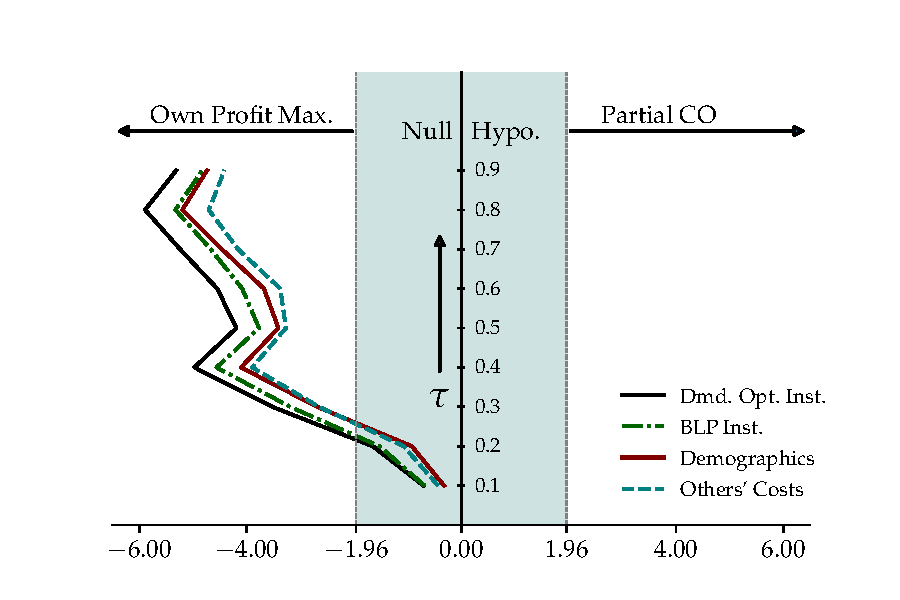
\includegraphics[width=10cm]{figures/tau_figure2.pdf}
\end{center}
\end{frame}

\begin{frame}[plain]{Stepping Back}
\begin{itemize}
\item In order to evaluate the common ownership hypothesis, we developed a conduct testing procedure building on the identification results of Berry and Haile (2014)
\pause \item Have another specification of common ownership? We can test any pair of models such that
\begin{enumerate}
\item Are fully specified, i.e. predict markups.
\item Yield distinct markups ($\Delta\eta \neq 0$).
\item We have instruments that are relevant to $\Delta \eta$, excluded from the supply function $h_s(\cdot)$, and mean independent of $\omega^0$.
\end{enumerate}
\pause
\item Note that this is not specific to common ownership
\begin{itemize}
\item Cartels: collusive versus oligopoly pricing? 
\item Vertical contracts: DM  or manufacturer pricing?
\item Labor: monopsony versus perfectly competitive labor markets?
\item Behavioral: suboptimal versus rational pricing rules?
\end{itemize}
\end{itemize}
\end{frame}

\begin{frame}[plain]{Wrapping Up}
Takeaways:
\begin{itemize}
\item Equilibrium markups are a nonlinear function of everything in the model. Using the model to get that nonlinearity right makes for a more powerful conduct test.
\item In RTE cereal, we see strong evidence in favor of own-profit maximization rather than common ownership pricing.
\item Discussion
\begin{itemize}
    \item We reject evidence of CO short-run price comepetition in RTE Cereal.
    \item Can't reject other mechanisms (CEO's living the quiet life)
    \item Can't explain stock market pricing anomalies
    \item In some sense CO is what we would see absent agency problems, so where are they?
\end{itemize}
\end{itemize}
\end{frame}


\section{Thanks!}
%------------
% APPENDIX
\appendix

\begin{frame}[plain]{Cereal Data: Prices}
\begin{center}
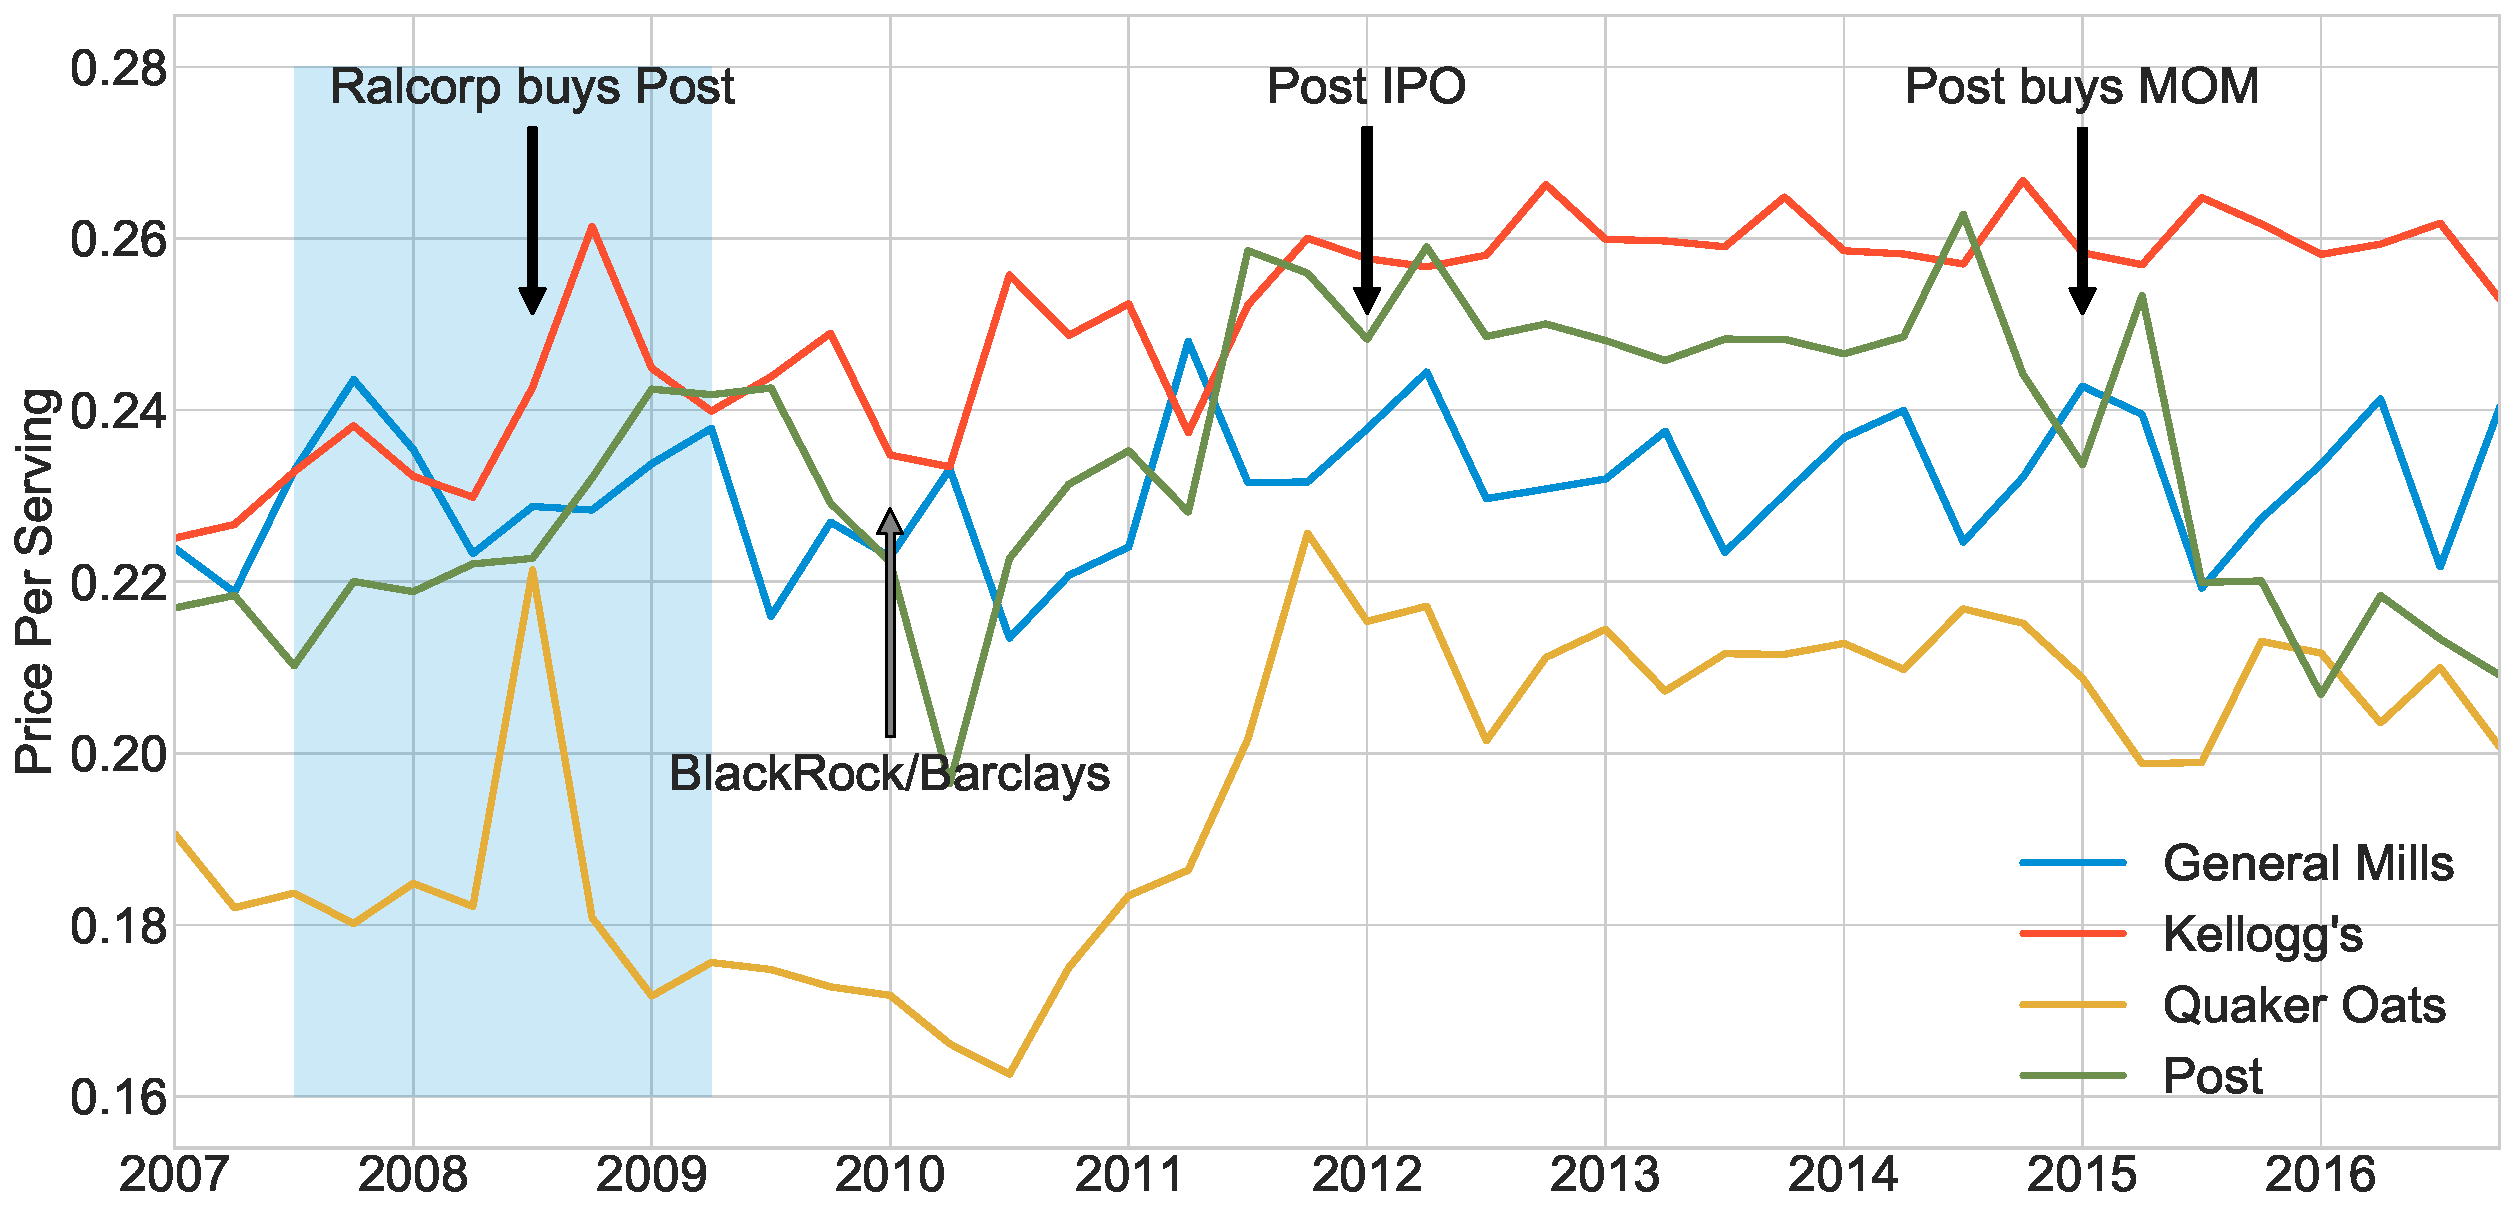
\includegraphics[height = 0.9\textheight ]{figures/firm_prices.pdf}
\end{center}
\end{frame}


\begin{frame}{Model Free Evidence?: Raisin Bran}
\begin{center}
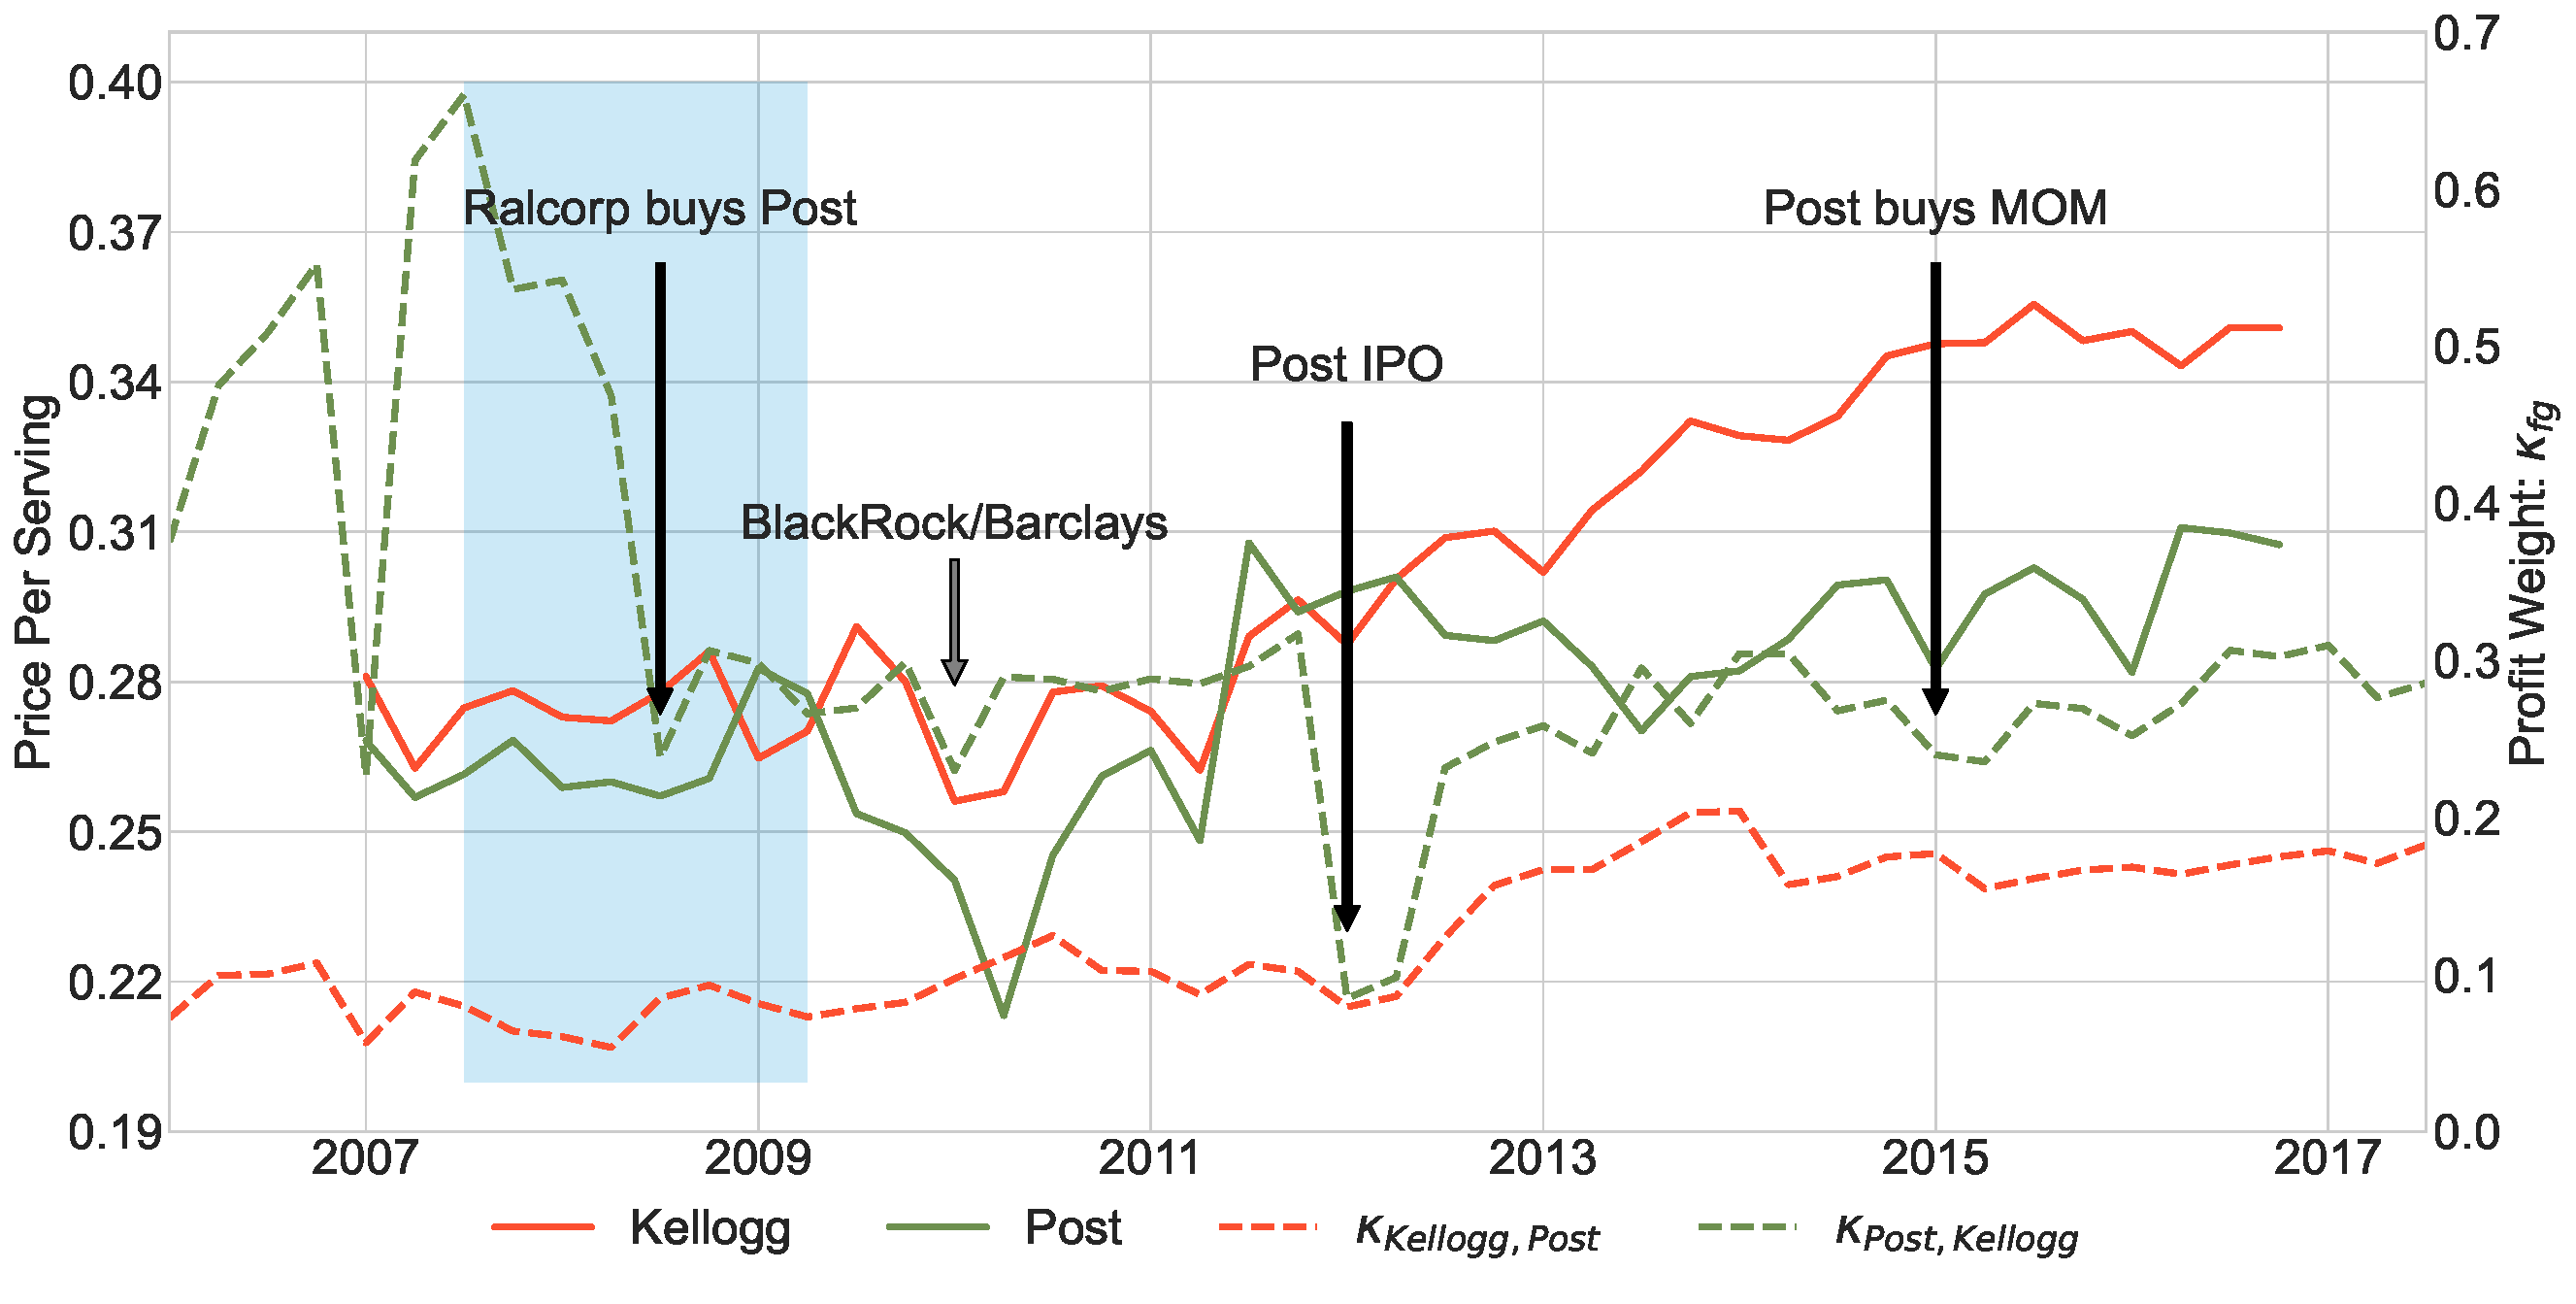
\includegraphics[height = 0.9\textheight ]{figures/raisin_bran.pdf}
\end{center}
\end{frame}


\begin{frame}[plain]{Cereal Data: Input Prices}
\begin{center}
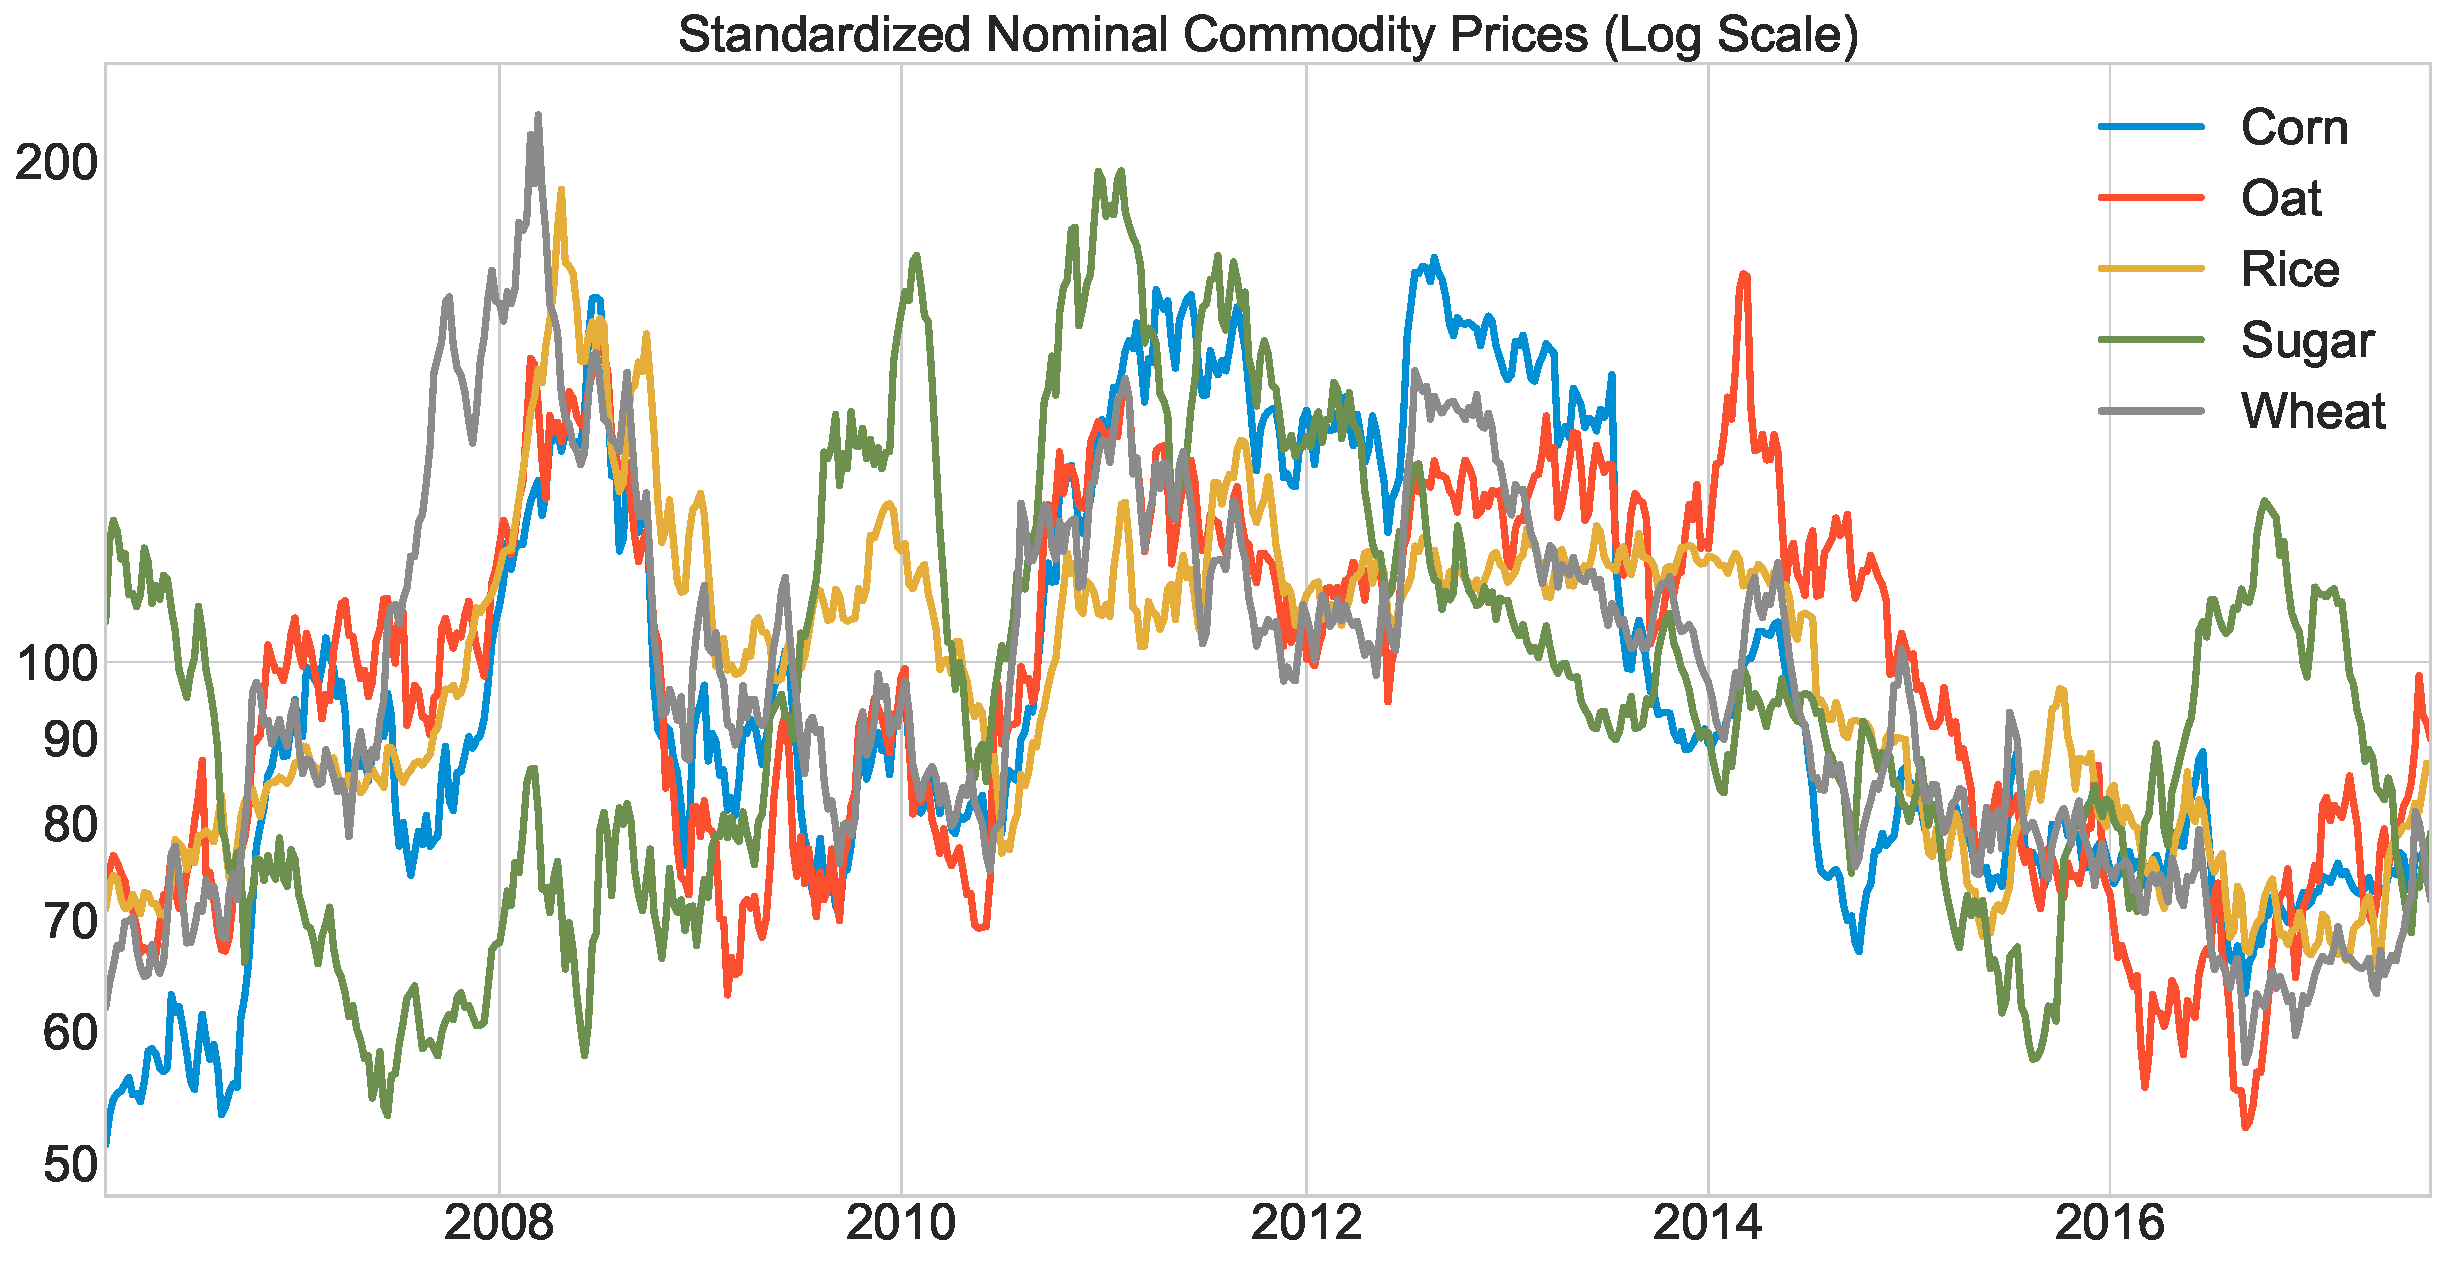
\includegraphics[height = 0.9\textheight ]{figures/input-prices.pdf}
\end{center}
\end{frame}


\begin{frame}[plain]{Cereal Data: Concentration}
\begin{center}
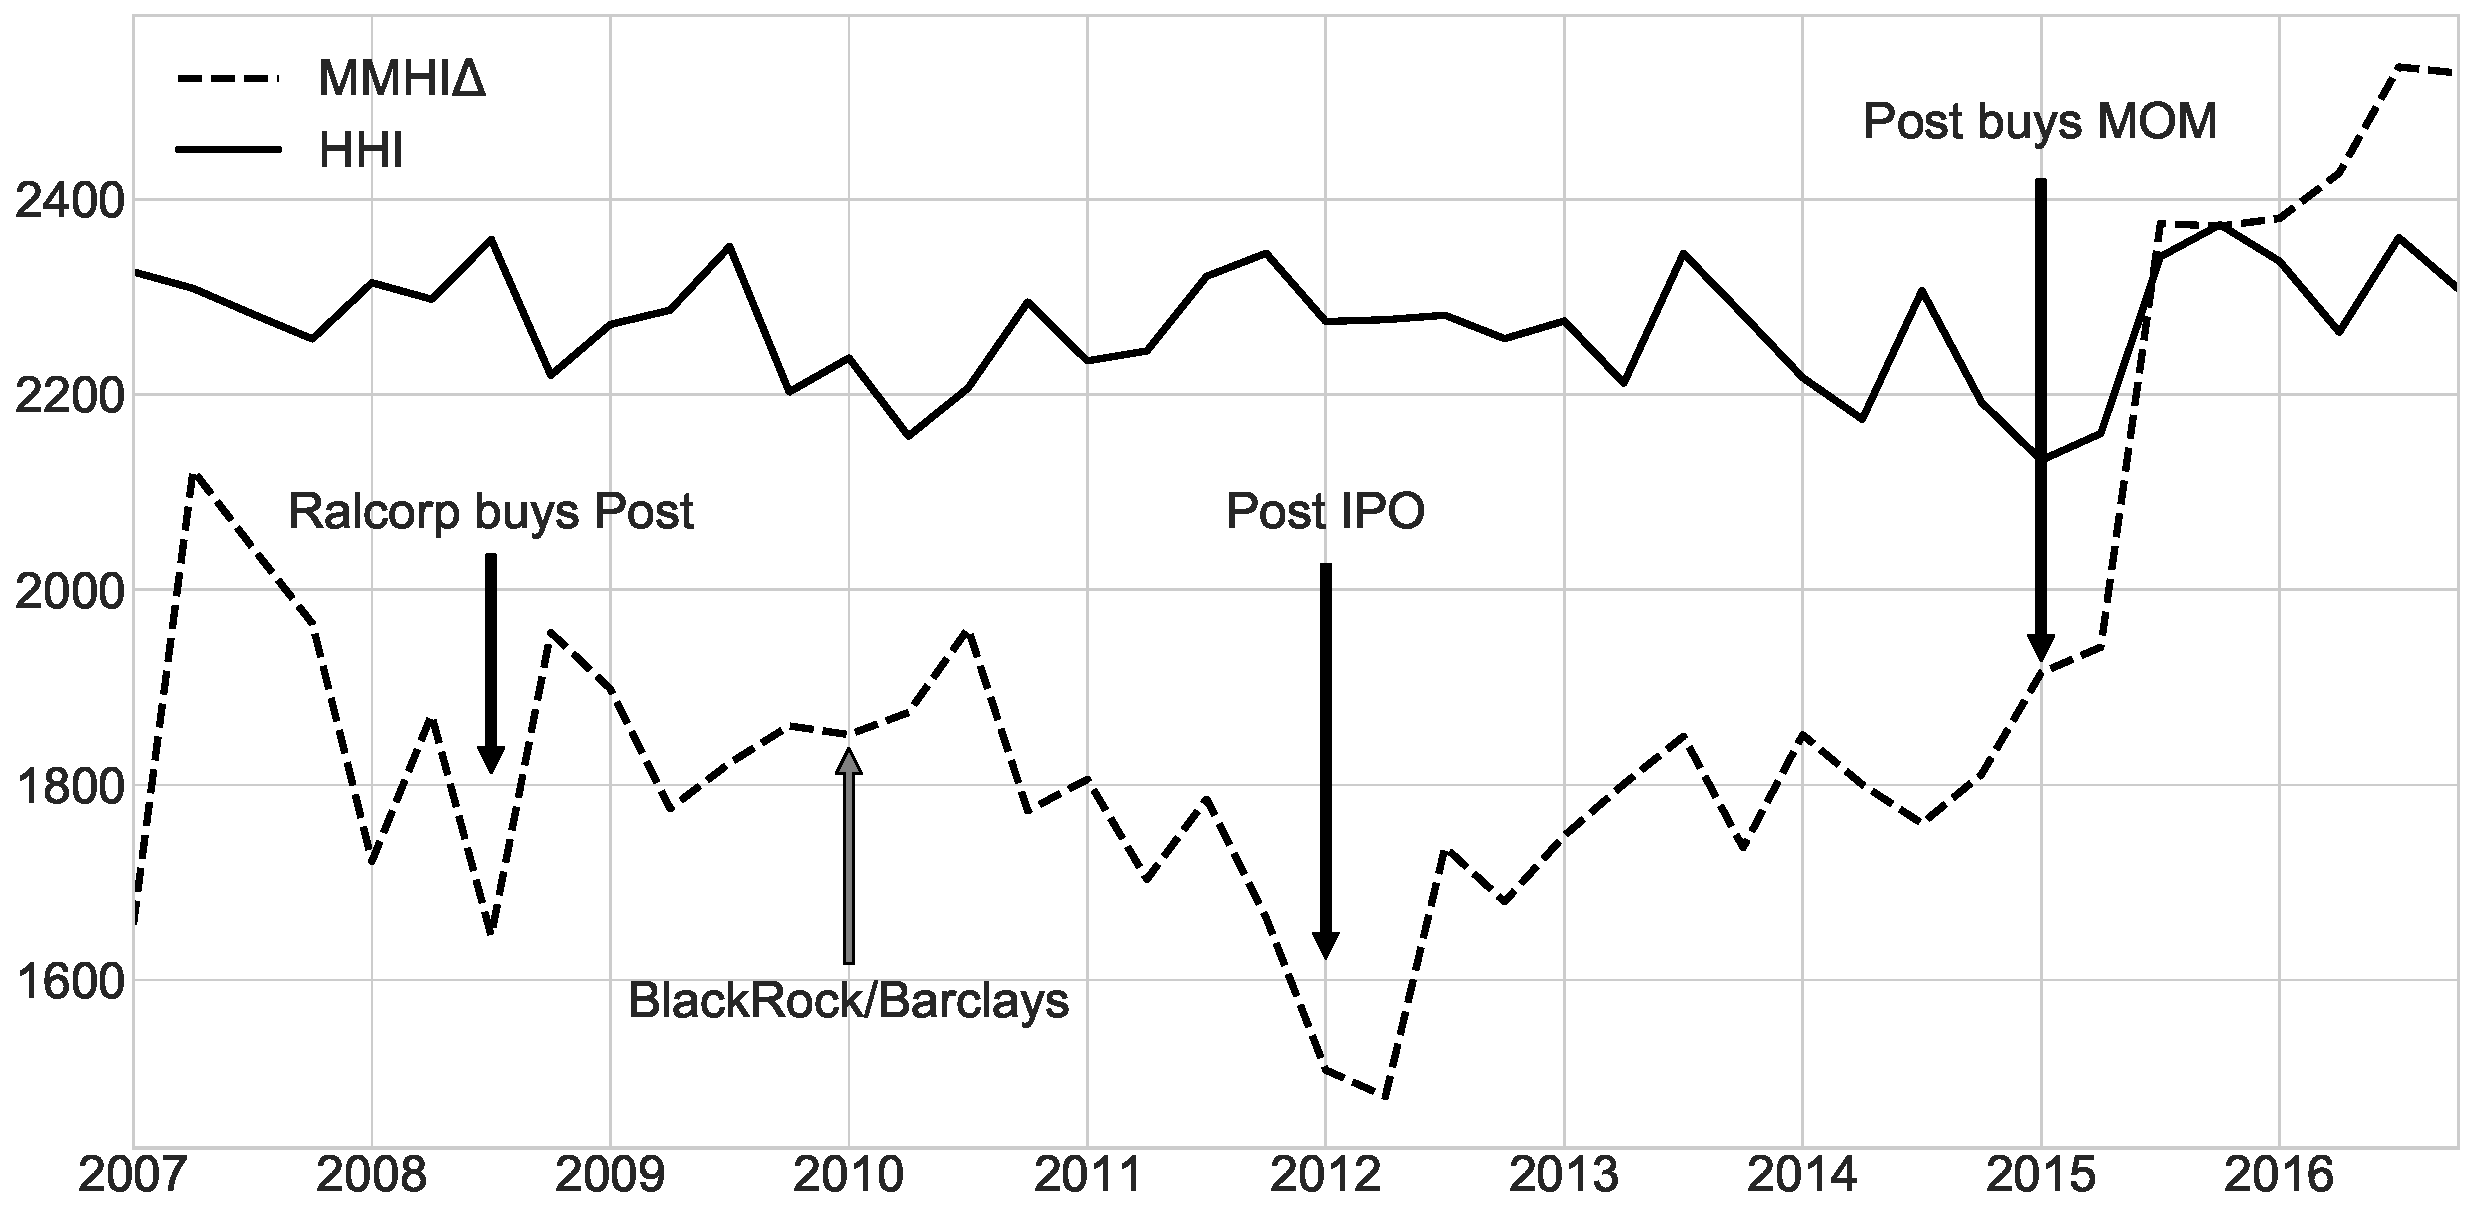
\includegraphics[height = 0.9\textheight ]{figures/all_mhhi_hhi.pdf}
\end{center}
\end{frame}



\end{document}
